\documentclass[12pt, twoside]{report}
\usepackage[a4paper, margin=3.3cm]{geometry}
\usepackage[english]{babel}
\addto\captionsitalian{\renewcommand{\abstractname}{Abstract}}
\usepackage{caption}
\usepackage{subcaption}
\usepackage{ragged2e}
\usepackage{hyperref}
\usepackage{booktabs} %per tabelle
\usepackage{siunitx}

%per diagrammi
\usepackage{tikz}
\usetikzlibrary{shapes.geometric, arrows.meta, positioning, fit, backgrounds}
\usepackage{amsmath}
\usepackage{amssymb}
\usepackage{lipsum}
\usepackage{fancyhdr}
\usepackage[backend=biber, style=numeric]{biblatex}
\usepackage{csquotes}
%\bibliographystyle{unsrt}
\usepackage{graphicx}
\usepackage{listings}
\usepackage{xcolor}
\graphicspath{ {./images/} }

\definecolor{codegreen}{rgb}{0,0.6,0}
\definecolor{codegray}{rgb}{0.5,0.5,0.5}
\definecolor{codepurple}{rgb}{0.58,0,0.82}
\definecolor{backcolour}{rgb}{0.95,0.95,0.92}

\lstdefinestyle{mystyle}{
    backgroundcolor=\color{backcolour},   
    commentstyle=\color{codegreen},
    keywordstyle=\color{magenta},
    numberstyle=\tiny\color{codegray},
    stringstyle=\color{codepurple},
    basicstyle=\ttfamily\footnotesize,
    breakatwhitespace=false,         
    breaklines=true,                 
    captionpos=b,                    
    keepspaces=true,                 
    numbers=left,                    
    numbersep=5pt,                  
    showspaces=false,                
    showstringspaces=false,
    showtabs=false,                  
    tabsize=2
}

\lstset{style=mystyle}
\addbibresource{references.bib}
\fancyhead[LE, RO]{\thepage}
\fancyhead[RE]{\leftmark}
\fancyhead[LO]{\rightmark}
%\fancyfoot[LE, RO]{\thepage}
\fancyfoot[CO, CE]{}

% STEP 1: include the package
\usepackage{uninafrontespizio}
% STEP 2: Front-page configuration
\Universita{Università degli Studi di Napoli Federico II}
\Facolta{Scuola Politecnica e delle Scienze di Base}
\Dipartimento{Dipartimento di Ingegneria Elettrica e Tecnologie dell'Informazione}
\CorsoDiLaurea{Corso di Laurea Magistrale in Automazione e Robotica}
%\AnnoAccademico{Anno Accademico 2022-2023}
\Titolo{MPC-based two-drone teleoperation architecture for exocentric vision}
\Relatore{Mario \textsc{Selvaggio}}
\Correlatori{Marco \textsc{Cognetti} \\Simone \textsc{D'Angelo}}
\RelatoreLabel{Relatore} %optional, default: Relatore
\Candidato{Alessandro \textsc{Cocchia}} %only one candidate is currently supported
%\CandidatoLabel{Candidata} %optional, default: Candidato
\Matricola{P38/000154}
\Logo{logo-federico-II.pdf} %path to logo image
\LogoWidth{4cm} %optional, default: 3cm
\LogoPosition{below-uni} % or top, or below-title, or above-title, or no-logo



\begin{document}
    % STEP 3: use \makefrontpage and/or \makefrontpagealt
    
\begin{titlepage}

\pagestyle{empty}
\makefrontpage

\end{titlepage}
    \nocite{*}
    \pagestyle{empty}
    \tableofcontents
    %\pagestyle{fancy}
    \abstract
\justify
In aerial robotics, shared control is widely exploited in contexts where high-level decision-making capabilities provided by the human are required and, at the same time, robot can assist human operator in performing the task in a safe and efficient way. In some cases, like complex inspections, the execution of semi-autonomous tasks via aerial robotics is obstructed by the limited situational awareness provided by onboard first-person view cameras. For this reason it could be useful to use two UAVs (Unmanned Aerial Vehicles): one (Inspection Drone) effectively acting for the inspection task, the other one (Observer Drone) as visual aid for the human operator. In this context, teleoperation can been used to let the operator intervene on both drones for actively monitoring the navigation and inspection, so to improve general safety and task performance. Because of all difficulties that arise from teleoperating two drones, the architecture features a shared-control paradigm. Precisely, this thesis proposes a human-robot shared control framework utilizing a two-UAVs architecture, exploiting \textit{exocentric vision} (i.e., third person view) to feed the human with the "best" view of the scene.
\\To achieve this, the observation task of Observer UAV is formulated as a nonlinear programming problem and solved via Nonlinear Model Predictive Control (NMPC). The NMPC controller minimizes the geometric 3D tracking error to keep observed UAV in the field of view at a desired relative distance, with a desired point Of view. Moreover, to prevent operator motion sickness, the controller explicitly minimizes acceleration, jerk and snap, ensuring smooth camera motion while respecting actuation constraints (thrust and torques). The framework features bilateral teleoperation: if human commands on Observer UAV try to crash it over the other drone or loose it from the view, a force feedback based on repulsive artificial potential field method is generated to guide the operator, without mathematically altering human command. Simultaneously, the Inspection UAV can perform an inspection task executing the contact utilizing an admittance filter planner. Human operator can perform the interaction through teleoperation, relying on the admittance filter that provides compliance to the drone during contact. 
\\Simulations to validate this architecture are conducted in Gazebo, using ROS2 middleware and PX4 firmware on the two drones. Simulation results demonstrate the real-time computational feasibility of the NMPC solver at 100 Hz and highlight a bounded geometric tracking error, ensuring the target is never lost from the FOV even under conflicting human inputs. The framework provides contact stability for the Inspection UAV and proves the effectiveness of haptic feedback in safely integrating human high-level decision-making with autonomous low-level constraints. 
\\Preliminary experiments have been conducted, validating simulation results only  over the Observer UAV, showing the effectiveness of NMPC controller and bilateral teleoperation in real scenarios, with a light sim-to-real gap. 
    \chapter{Introduction}
    %Importanza della robotica aerea nell'ambito degli interventi di esplorazione e di ispezione di luoghi difficillmente accessibili all'essere umano o pericolosi per esso
%\\Spesso in queste situazioni si preferisce delegare un certo grado di autonomia al robot ed all'occorrenza l'essere umano può intervenire facendo teleoperazione.
%\\Lo scenario pensato è quello di 2 droni, di cui uno deve compiere un task che è stato pensato come peg-in-hole, ad all'interno di un pilone di un ponte, e l'altro deve fornire un punto di vista all'essere umano inquadrando costantemente l'altro drone.
%\\ I droni sono entrambi quadricotteri, per cui sottoattuati per loro natura nello spazio 3D. Per questo motivo il problema viene affrontato nel seguente modo: entrambi i droni prevedono l'utilizzo di PX4 come firmware per la gestione di basso livello; il drone che effettua il task viene controllato in posizione, usando i controllori di bordo standard di PX4; l'altro drone è controllato direttamente in thrust e torque e pianifica in real-time una traiettoria ottima tramite un framework MPC in modo da ottimizzare diversi obiettivi, tenendo conto allo stesso tempo dei vincoli di attuazione del drone. Nel contempo l'operatore umano può effettuare teleoperazione in 2 modi possibili: agendo sul drone che osserva, cambiandone ad esempio il punto di vista dinamicamente, o agendo sul drone che effettua il task, ad esempio proprio per effettuare egli stesso il task di inserzione. 

Nowadays, aerial robotics has become an established tool for operations in hazardous and degraded environments. The use of Unmanned Aerial Vehicles (UAVs) allows for the substitution of human operators in high-risk areas, which is particularly relevant for the inspection and maintenance of aging civil infrastructure. In these scenarios, robotic platforms are deployed to collect data and perform non-destructive measurements, reducing human exposure to dangerous conditions while accessing confined or structurally compromised spaces.
Despite the push towards full autonomy, unstructured real-world environments often require a human-in-the-loop architecture. In such systems, the robot handles low-level stabilization and task execution, while the human operator provides high-level cognitive decision-making skills. To operate effectively, the remote pilot requires a high degree of situational awareness. Relying exclusively on an onboard (egocentric) camera often limits this awareness, especially during close-proximity operations or physical interactions with the environment. This is even more true when having a fixed camera over an underactuated drone. An exocentric point of view, provided by an external observer, maximizes the operator's understanding of the spatial relationship between the interacting robot, the structural constraints, and potential obstacles. Furthermore, to prevent motion sickness and ensure the transmitted video stream is usable for remote decision-making, the observer platform must guarantee smooth and stable camera framing.
\section{Context and Motivations}
\begin{figure}
    \centering
    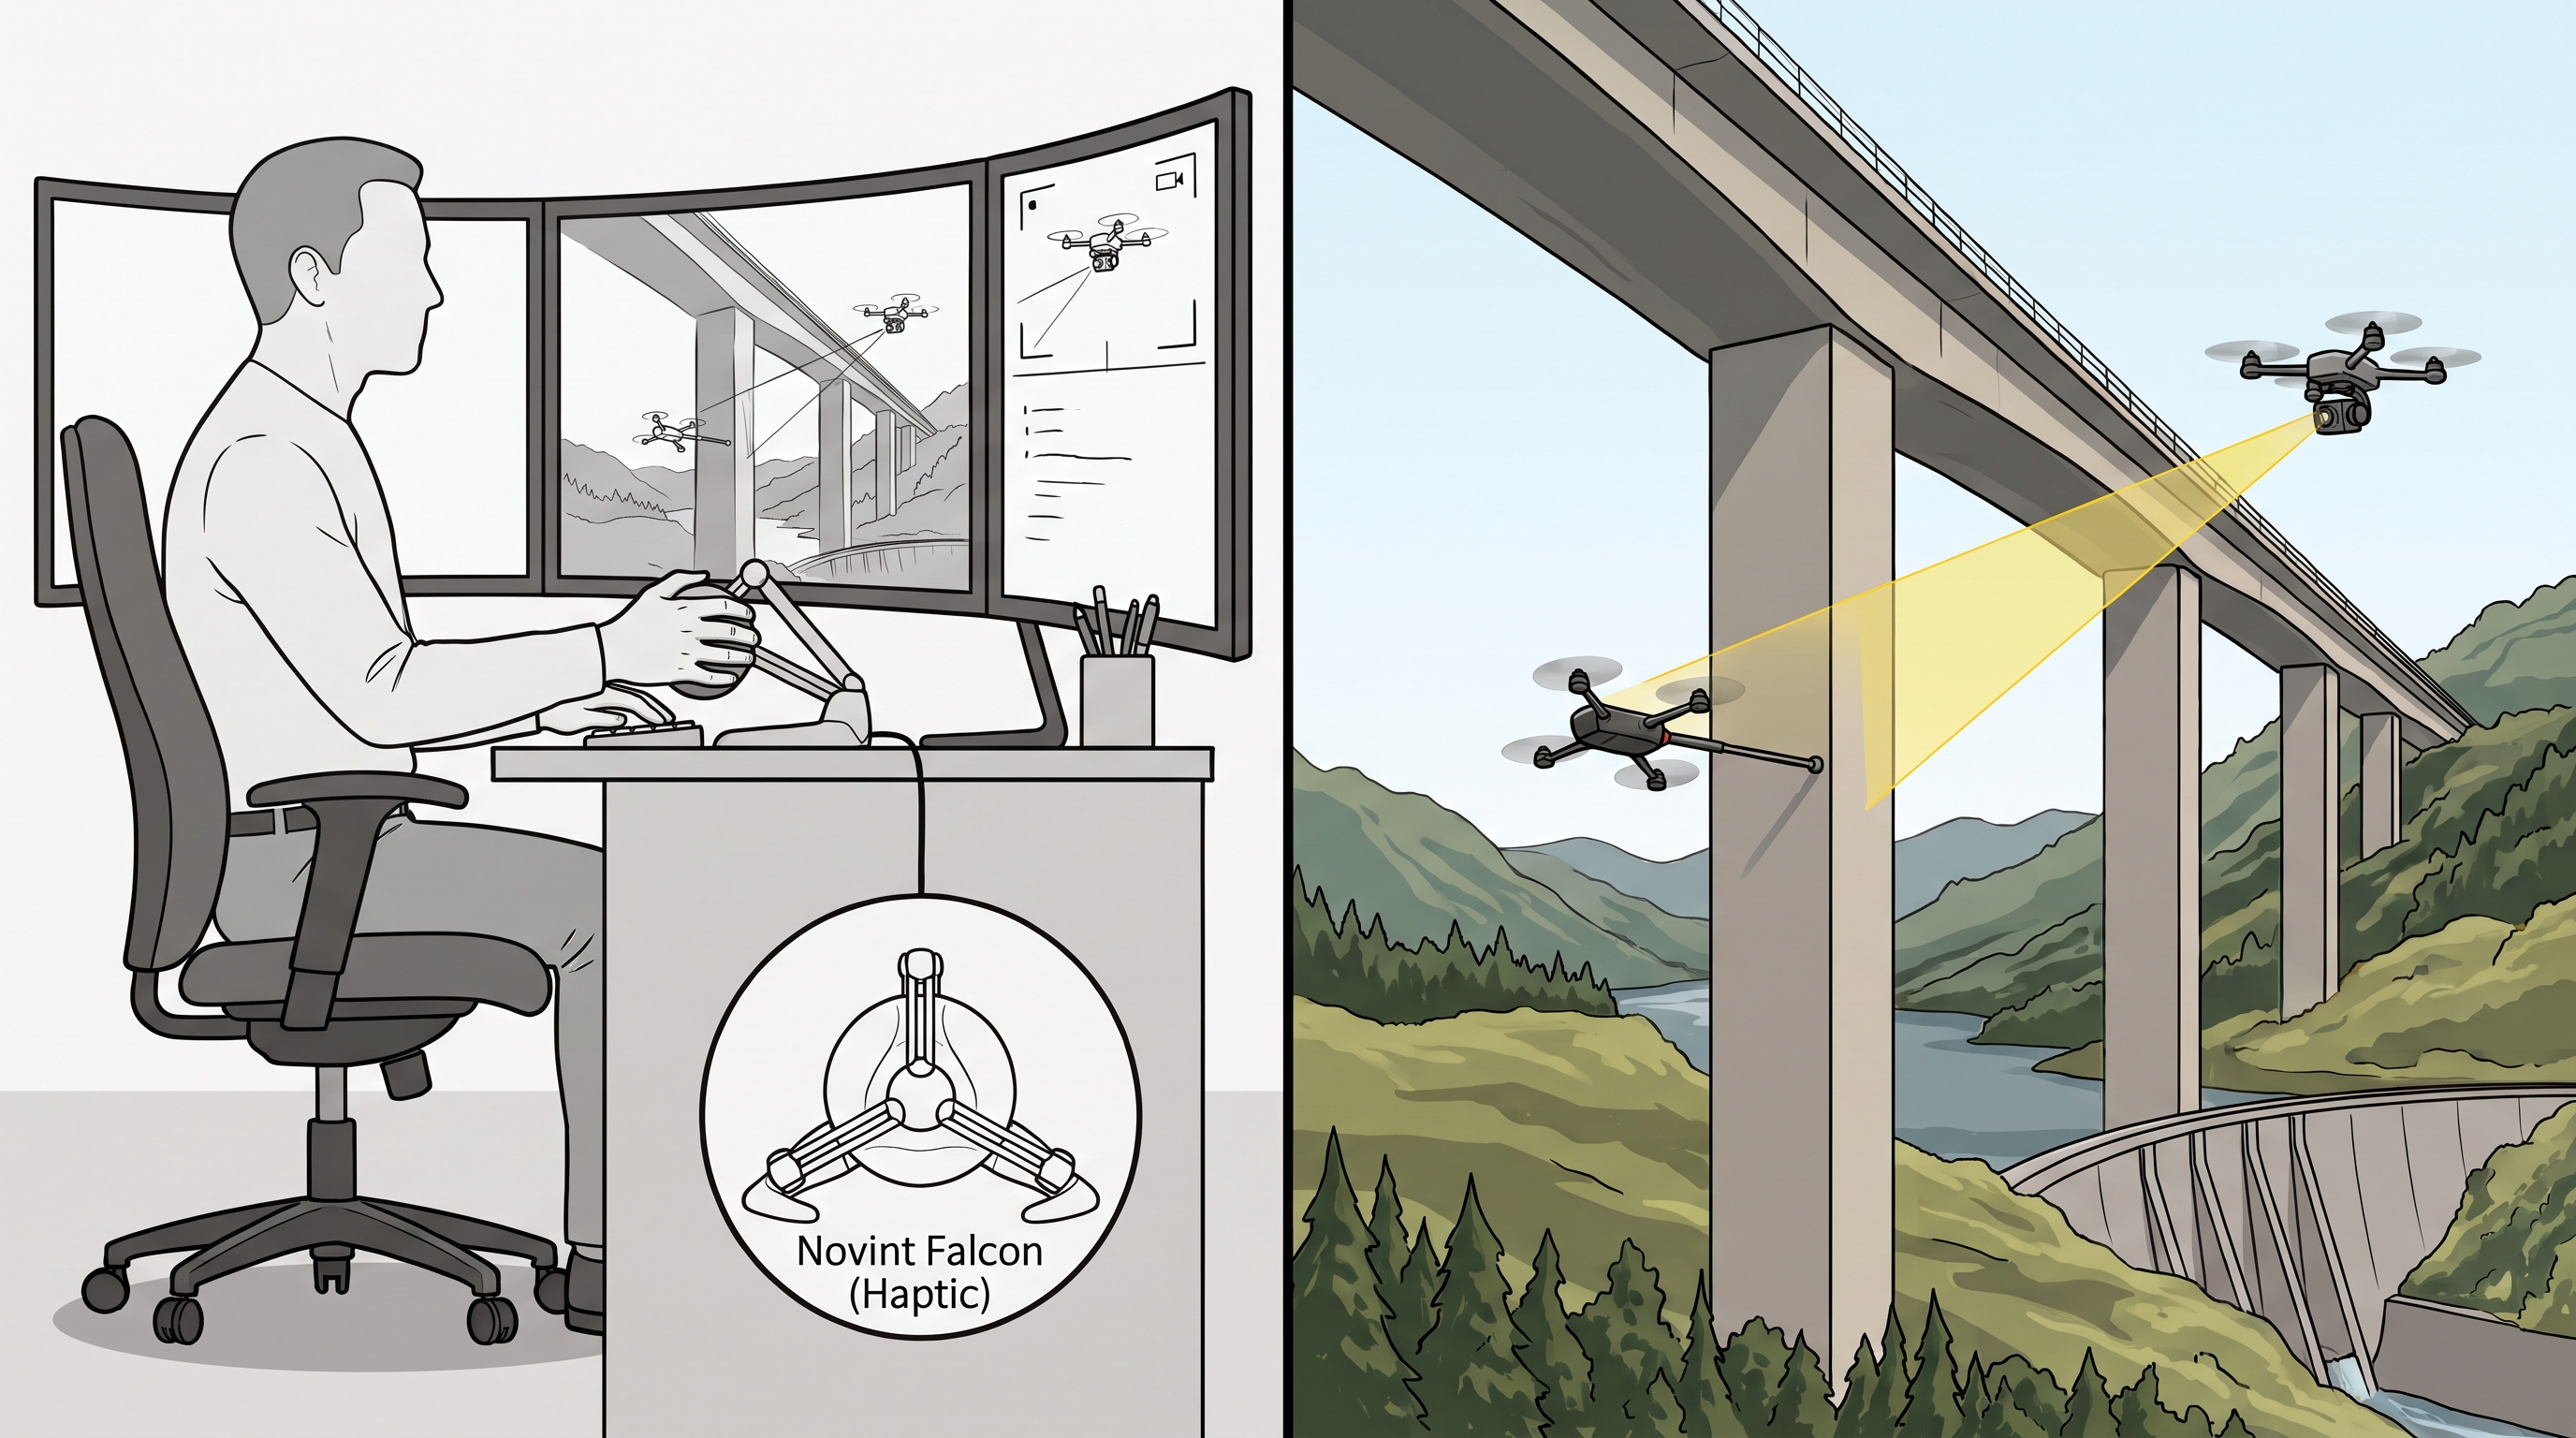
\includegraphics[width=0.8\linewidth]{Immagini/Capitolo1/scenario_introduction.jpeg}
    \caption{Scenario: observer drone frames contact inspection task performed by inspection drone; human operator can command inputs to both drones via haptic device}
    \label{fig:placeholder}
\end{figure}
The thesis addresses a cooperative aerial mission designed for the inspection of confined environments, such as the interior of a bridge pillar. The system relies on a dual-quadrotor setup: an inspection drone tasked with performing a controlled contact with the structure, and an observer drone tasked with providing an optimal exocentric view of the operation.
\\To manage the unpredictability of the environment and the highest precision in inspection contact, a haptic teleoperation interface is integrated into the system, allowing the operator to intervene on two different levels. On one hand, the operator can take command of the observer drone to dynamically change the point of view in the event of occlusions, loss of situational awareness, or unforeseen obstacles. On the other hand, the operator can switch control to the inspection drone to manually guide the final contact phase, compensating for physical uncertainties that the autonomous system cannot resolve.
\section{Contributions}
To support this shared-control paradigm, a multi-layered control and planning framework has been developed.
The core contribution involves the control architecture for the observer UAV, which must satisfy multiple requirements: tracking an unknown and dynamic trajectory of the inspection drone, keeping the target framed, avoiding motion sickness in human operator and responding online to the viewpoint changes commanded by the operator via the haptic device.
To achieve this despite the inherent underactuation of quadrotors, a Nonlinear Model Predictive Control (NMPC) scheme has been designed. The NMPC optimizes the camera framing while ensuring safety by respecting actuation constraints, acting directly at a thrust and torque level and minimizing higher-order time derivatives in the cost function. Moreover, to compensate for external disturbances and model mismatches, a MBE (Momentum Based Estimator) is updated online, making the control intrinsically robust.
\\On the other hand, the inspection UAV operates using a position control strategy modified with an admittance filter to ensure a stable execution of the physical contact.
\\Human is inserted inside the loop through bilateral teleoperation over NMPC observer UAV and unilateral teleoperation to the interacting one, bringing the framework into Shared Control.
\\Everything is orchestrated by a FSM that decides which are the best views for the human according to FSM state and handles emergencies.
\\To guarantee system reliability and facilitate a realistic transition to hardware, the entire high-level control architecture for both platforms has been integrated with the standard and open-source \texttt{PX4} autopilot firmware.

\section{Thesis Outline}
The here presented thesis  is structured as follows. 
Chapter 2 reviews the state of the art concerning shared control architectures, vision modalities in teleoperation, and online planning and control methods for aerial robotics. 
Chapter 3 defines the problem statement and presents an overview of the proposed dual-UAV system architecture, detailing the exocentric vision paradigm, the contact inspection requirements, and the sequential phases of the cooperative mission. 
Chapter 4 provides the mathematical formulation of the problem. It details the rigid body dynamics of the quadrotors, the Non-linear Model Predictive Control (NMPC) framework designed for the observer drone's visual tracking, the human-robot shared control layer, together with the mathematical generation of haptic references and the Artificial Potential Fields (APF) used to render the force feedback to the operator and the admittance control scheme utilized by the inspection drone to manage physical interactions. 
Chapter 5 describes the software and hardware implementation of the overall framework. It covers the ROS 2 middleware integration, the PX4 flight stack interactions, the finite state machine governing the mission supervisor, and the real-time execution details of the NMPC and admittance nodes. 
Chapter 6 presents the simulation and experimental results, validating the control framework's performance, the tracking accuracy, and the effectiveness of the haptic shared control paradigm. 
Finally, Chapter 7 summarizes the conclusions of this work and outlines potential directions for future research.   
    \chapter{State of the Art}
    In recent years, the deployment of Unmanned Aerial Vehicles (UAVs) in high-risk scenarios and Non-Destructive Testing (NDT) has gained significant relevance in robotics research~\cite{siciliano2008springer}. Structural health monitoring tasks, such as the routine inspection of aging bridges and civil infrastructures, require reliable physical interaction for sensor positioning and structure monitoring, where aerial robots can effectively substitute human workers in hazardous and high-elevation workspaces~\cite{hao2024bilateral, dangelo2025semi_platform}. However, achieving fully autonomous execution in unstructured environments remains an open challenge due to environmental uncertainties, dynamic obstacles, and unexpected mission anomalies. 
\\To bridge the gap between human cognitive judgment and robotic execution, shared control (SC) and shared autonomy (SA) architectures have become the predominant paradigms~\cite{selvaggio2021autonomy}. Shared control allows a remote operator to take high-level decisions while the autonomous system remains stable and ensures constraint satisfaction. In bilateral teleoperation frameworks~\cite{hokayem2006bilateral}, incorporating haptic feedback provides the remote pilot with an intuitive physical rendering of environmental interaction forces and artificial safety barriers, as demonstrated by Hao et al.~\cite{hao2024bilateral} and D'Angelo et al.~\cite{dangelo2025semi}. 
\\Despite the advantages of shared control, performing aerial contact tasks is heavily constrained by perceptual limitations. Traditionally, aerial teleoperation relies on an egocentric perspective, where the operator supervises the scene exclusively through an onboard First-Person View (FPV) camera. During physical contact maneuvers against vertical surfaces, this perspective inevitably leads to total visual occlusion, complete loss of 3D depth perception and loss of situational awareness. Furthermore, standard underactuated quadrotors must tilt to move and to exert forces, causing significant video shake and induced motion sickness for the human operator. As demonstrated by ~\cite{uhde2024allocentric} in multi-robot coordination, shifting from an egocentric to an allocentric (or exocentric) perspective drastically reduces the operator's cognitive load, eliminates occlusions, and restores proper spatial understanding.
\\To provide an active exocentric perspective, the observing aerial platform must continuously replan its trajectory to keep the interacting agent inside its Field of View (FOV). Model Predictive Control (MPC) represents the established standard in the literature to solve constrained multi-objective aerial tracking problems. Works like~\cite{jacquet2021motor} demonstrated that perception-constrained Nonlinear MPC (NMPC) can explicitly enforce camera FOV limitations while simultaneously respecting physical actuation bounds. Similarly, in~\cite{penin2018vision} it has been addressed reactive target tracking while preventing visual occlusions and in~\cite{shayan2025exponential} it has been demonstrated that predictive formulations incorporating jerk-level constraints ensure reactive yet remarkably smooth quadrotor motion.
\\Building upon these established standards, the framework developed in this thesis addresses the residual limitations of single-agent inspection systems. For this reason, instead of relying on a single aerial manipulator, the mission is decoupled between a dedicated Inspection UAV executing the physical contact and an Observer UAV acting as an active exocentric camera. This completely separates the video stream from contact vibrations and dynamic tilting.
\\Moreover, the proposed NMPC actively tracks a moving UAV and the optimization cost explicitly penalizes linear/angular accelerations, jerk, and snap, guaranteeing smooth camera movements specifically tuned to prevent operator visual fatigue. The NMPC directly commands body thrust and torques to the PX4 autopilot in offboard mode.
\\Also, the architecture incorporates online Point of View (PoV) adjustments commanded by the operator via a haptic interface. Here the geometric FOV boundaries and safety distances are mapped into continuous repulsive forces via Artificial Potential Fields (APF), guiding the operator away from visual loss without overriding their commands.
\\For the inspection drone, stable surface contact is achieved through a high-level admittance filter, ensuring compliant interaction on standard underactuated platforms without requiring complex tiltable hardware.

    \chapter{System Overview}
    %SPIEGARE SETUP E PROBLEMI (2 droni, haptic, problemi che ci sono in quest'ambito)
This chapter presents the architecture of the proposed two-drone framework and clarifies the main technical challenges addressed. 
\\Aerial robotics is a fundamental tool for operating in dangerous or degraded environments. UAVs are often used to keep human operators safe while performing non-destructive measurements on civil infrastructures. However, performing contact-based tasks requires a clear understanding of the workspace. When a drone approaches a structure, onboard First-Person View (FPV) cameras suffer from extreme occlusion and lack of depth perception. 
\\To overcome this limitation and maximize the human situational awareness, this thesis proposes an architecture centered around an active exocentric camera drone. In this setup, a second UAV acts as a target and performs the physical interaction with the environment. 
\\The observer drone must guarantee a stable video feed, avoiding any motion sickness for the human operator. At the same time, it must track a target drone whose trajectory is not known in advance. To solve this problem despite the underactuation of quadrotors, the system relies on a Non-linear Model Predictive Control (NMPC). This controller optimizes the camera framing and supports online POV adjustments commanded by the operator via a haptic device. 
\\Finally, the whole architecture is integrated with the standard PX4 firmware. Keeping the high-level logic connected to a known and tested flight stack provides reliable low-level stabilization and makes the transition to real hardware easier.

\section{Exocentric vision}
Using a standard onboard First-Person View (FPV) camera for physical interaction tasks presents some limitations. An egocentric perspective naturally compromises both the safety and the overall effectiveness of the mission.
When the inspection drone approaches a surface to make contact, the onboard camera ends up facing the wall from a very close distance. This completely blocks the Field of View (FOV). The human operator loses all environmental context, making it impossible to see surrounding obstacles or the actual position of the drone. An exocentric camera solves this simply by looking at the scene from the outside, keeping the full situational awareness intact.
\\Moreover, flying a drone toward a physical target using a flat, frontal 2D video feed makes it difficult to judge the remaining distance before impact. Depth perception is almost entirely lost. An observer drone tracking the operation from a lateral or isometric angle naturally restores this 3D spatial understanding, allowing the operator to clearly see the gap between the drone and the structure.
\begin{figure}[h!]
\centering
\begin{subfigure}[b]{0.49\textwidth}
    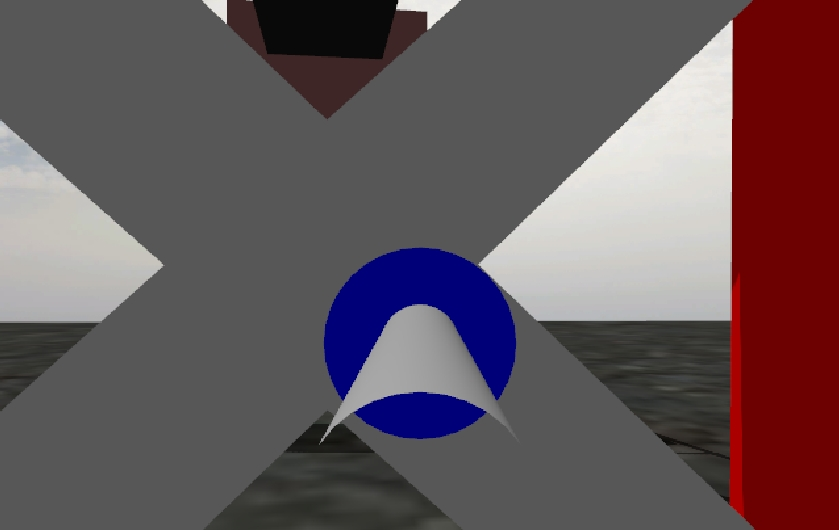
\includegraphics[width=\linewidth]{Immagini/Capitolo3/first_pov.jpg}
    \caption{Egocentric POV}
    \label{fig:first_pov_intro}
\end{subfigure}
\begin{subfigure}[b]{0.49\textwidth}
    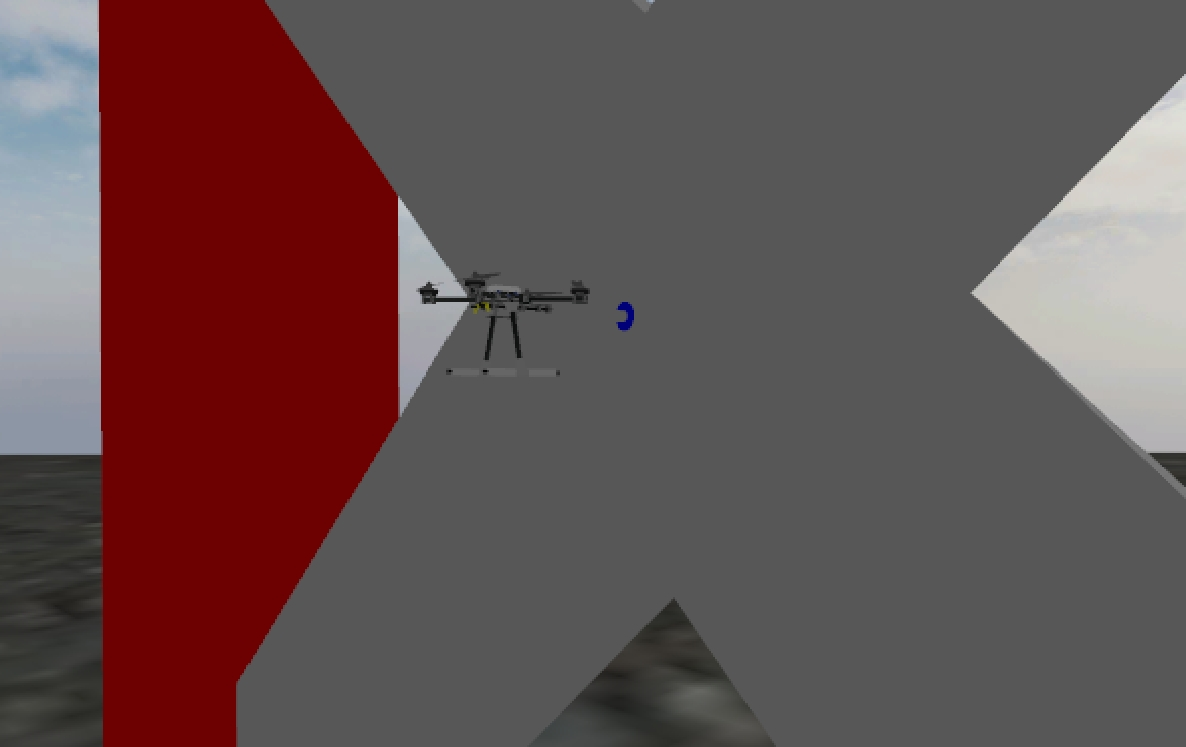
\includegraphics[width=\linewidth]{Immagini/Capitolo3/third_pov.jpg}
    \caption{Exocentric POV}
    \label{fig:third_pov_intro}
\end{subfigure}
\caption{Visual comparison between egocentric and exocentric views for bridge inspection task}
\end{figure}
\\Another major issue is the dynamic coupling of the quadrotor. Since standard quadrotors are underactuated, they must tilt to move or apply forces against a wall. If the camera is rigidly attached to the inspection drone, it will shake with every single pitch, roll, or contact vibration. The resulting video feed becomes chaotic, degrading the inspection quality and easily causing motion sickness for the operator. By using an independent observer drone, the visual task is completely decoupled from the physical one. The MPC can then focus entirely on planning a smooth and stable camera trajectory, isolating the operator from the rough dynamics the contact drone has to face.
\section{Shared control}
A fully autonomous operation is often unfeasible in unstructured environments. The human operator must be able to intervene during the mission. For this reason, a haptic device is integrated into the control loop. 
\\The operator uses the haptic interface for two main purposes. The first one is to dynamically change the Point of View (POV) of the observer drone. This intervention is necessary in case of sudden occlusions, unexpected obstacles, or a general loss of situational awareness. The operator can move the external camera to find a better angle without interrupting the tracking task. 
\begin{figure}
    \centering
    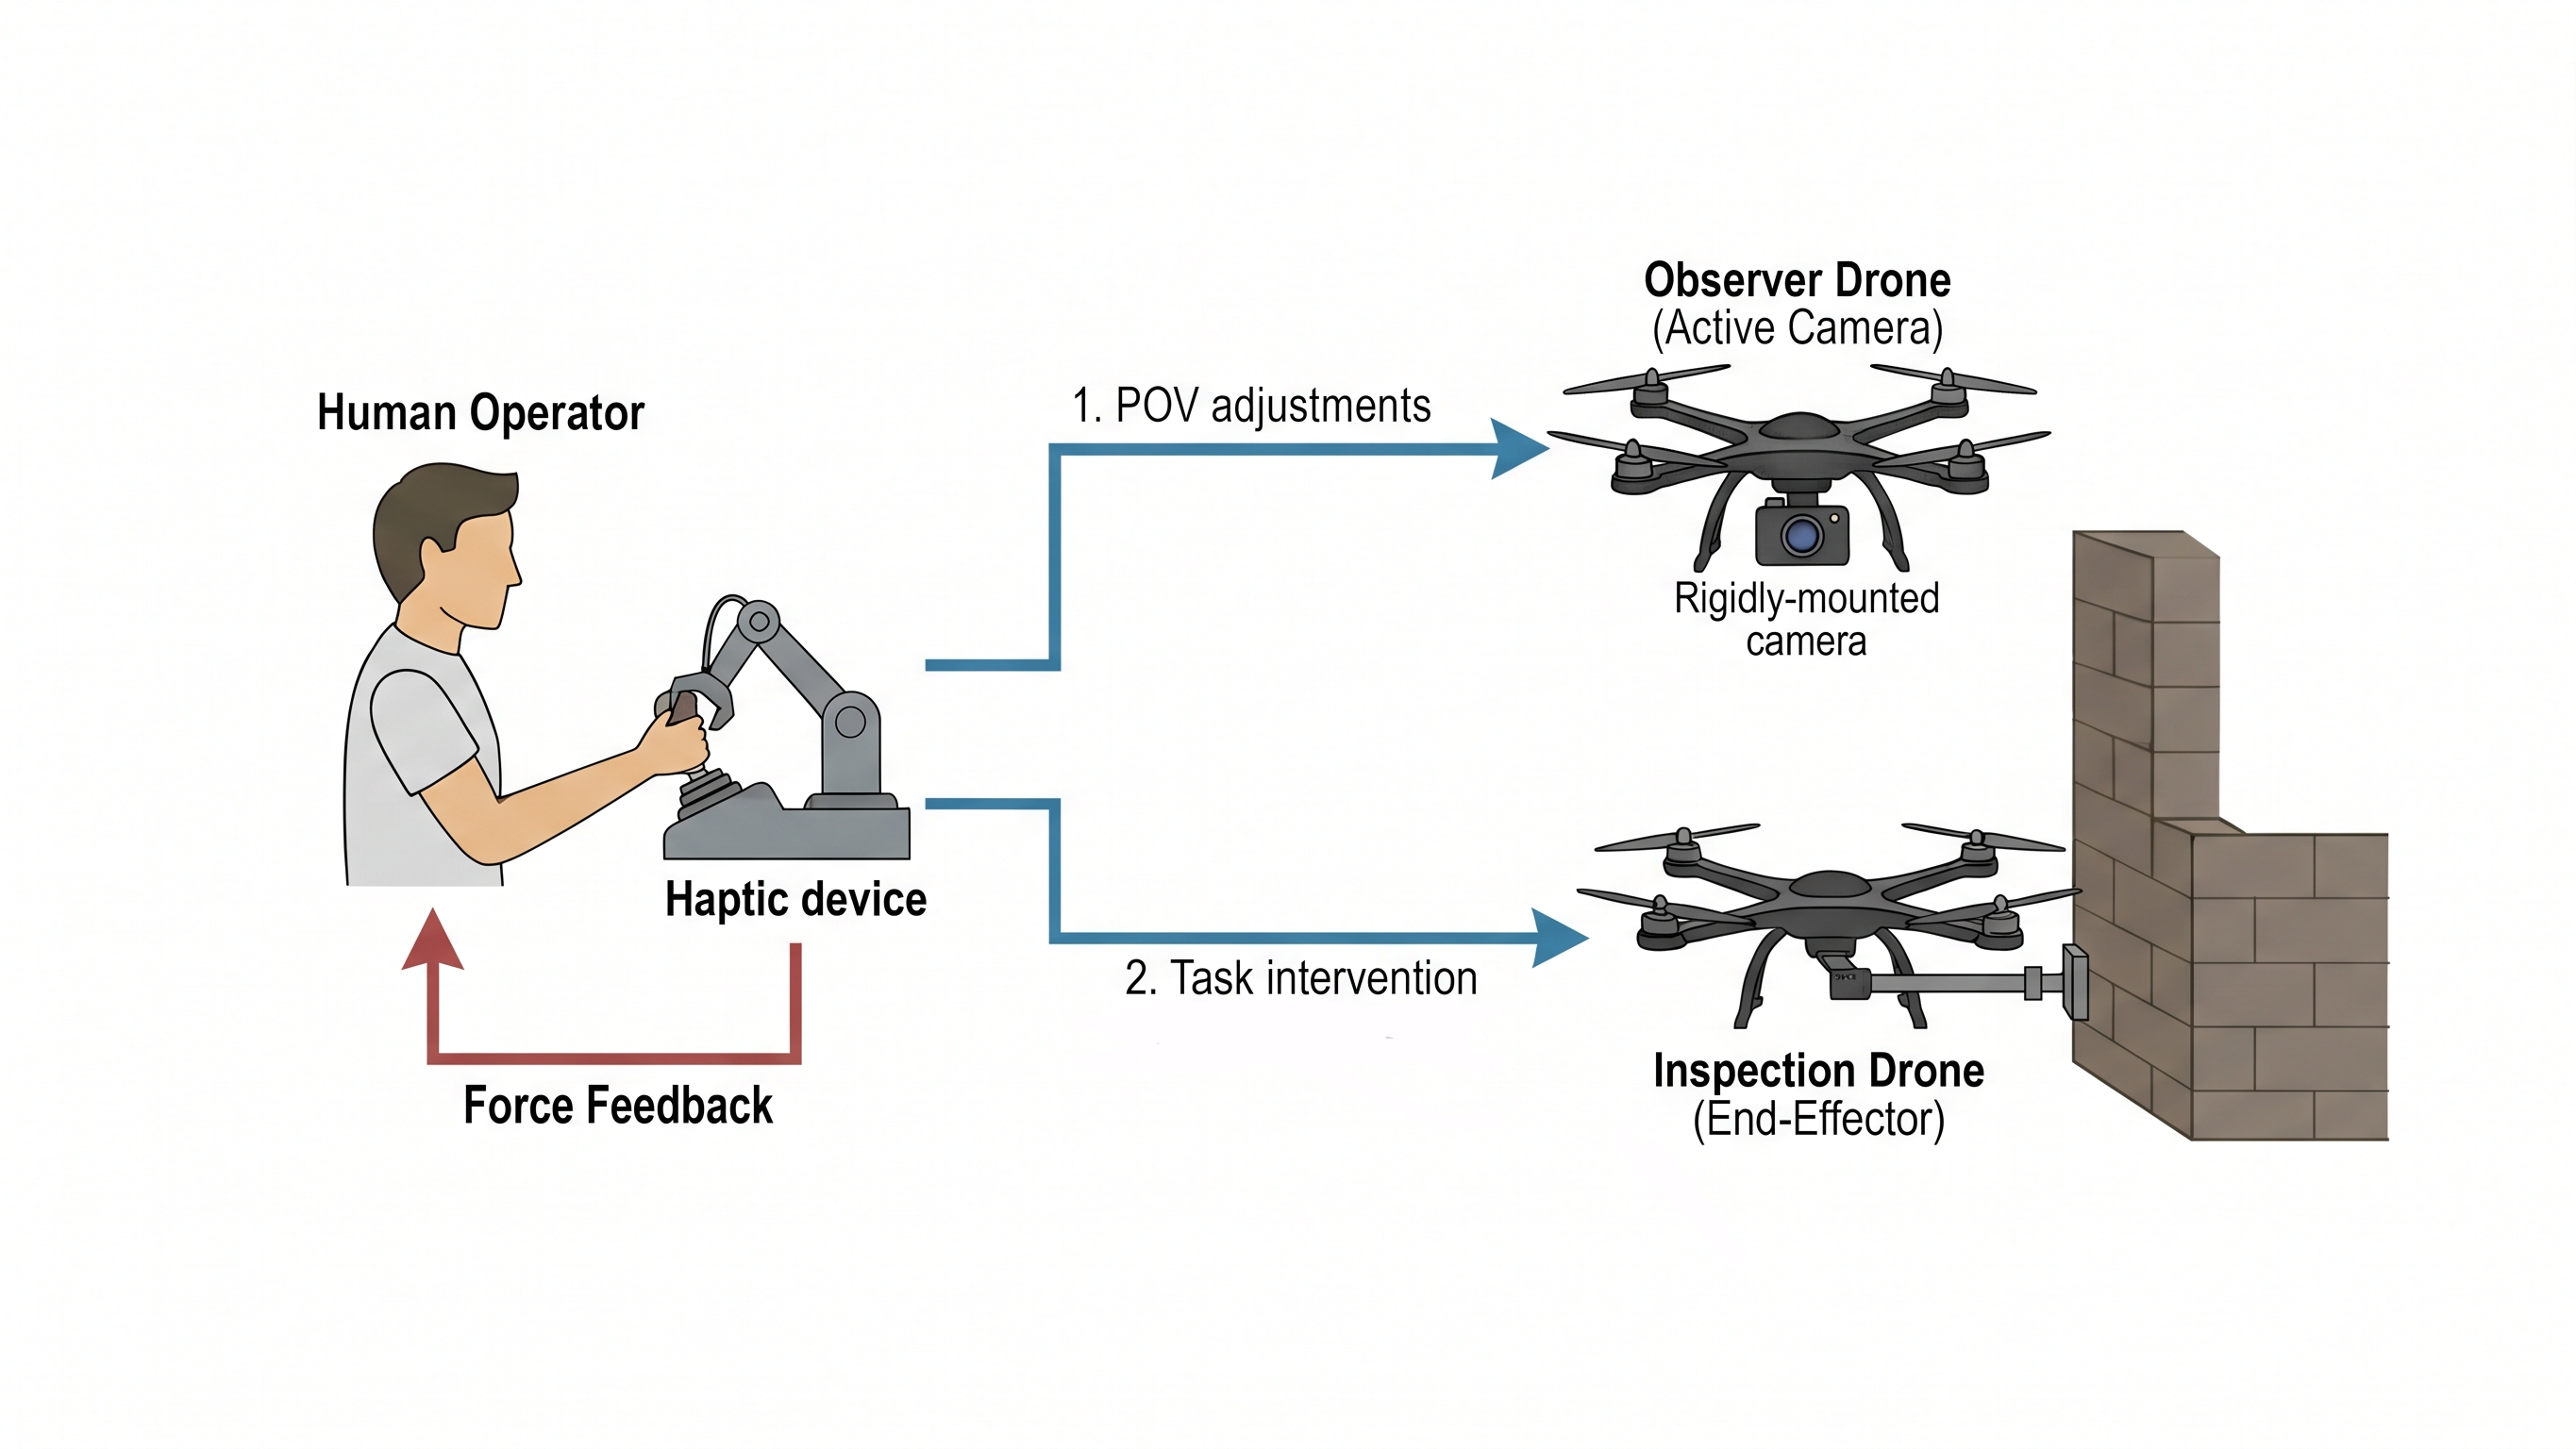
\includegraphics[width=\linewidth]{Immagini/Capitolo3/Shared Control.jpeg}
    \caption{Bilateral teleoperation illustration}
    \label{fig:shared_control_intro}
\end{figure}
\\The second purpose is to take direct control of the inspection drone. During the interaction phase of the mission, the operator guides the platform to perform the non-destructive measurements in a controlled way. In this case, the human decision-making is combined with the low-level admittance filter to maintain a stable contact with the wall.
\\Furthermore, the haptic device provides physical feedback to the user; for this reason we speak about \textit{bilateral teleoperation}. The mathematical limits of the camera field of view and the safety distances are translated into repulsive forces. This physical sensation prevents the operator from losing the target or crashing the drones.
\section{Contact inspection}
The execution of physical contact tasks with a multi-rotor platform introduces complexities with respect to standard free-flight navigation. When the inspection drone physically interacts with a rigid surface, such as a bridge pillar, it experiences environmental reaction forces. If the UAV is governed by a standard position controller, it will interpret the physical wall simply as a persistent position error, keeping pushing inside it. This mismatch causes the controller to aggressively increase its control input in an attempt to reach the unfeasible reference inside the wall, leading to violent inclination, actuator saturation, and potential crashes.
\begin{figure}[h!]
    \centering
    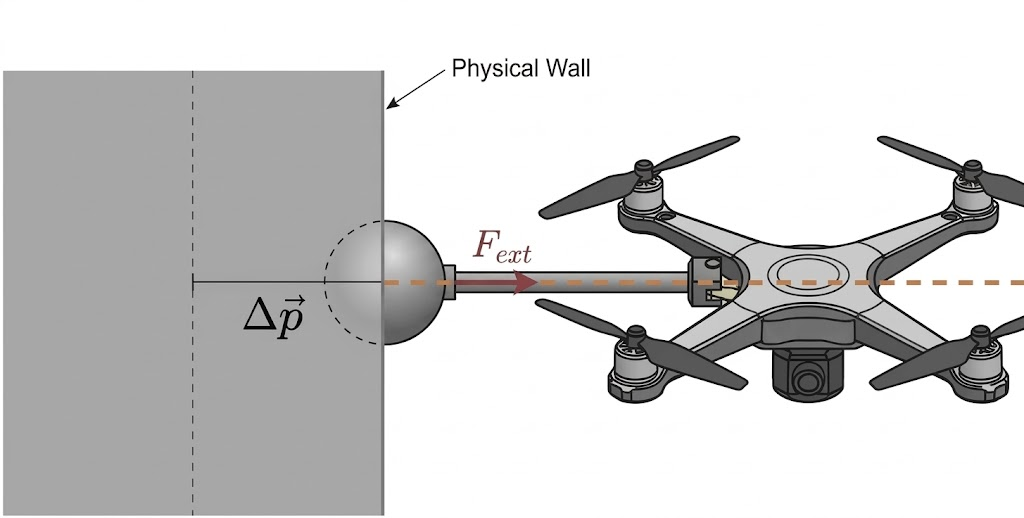
\includegraphics[width=0.5\linewidth]{Immagini/Capitolo3/Drone_interaction.jpeg}
    \caption{Drone interacting with environment; position goal behind the wall}
    \label{fig:interaction_intro}
\end{figure}
To safely manage this interaction, the architecture implements an admittance filter that makes the drone compliant with the environment, conceptually acting as a virtual spring-damper system. Instead of rigidly tracking a static geometric setpoint, the admittance framework translates the external contact forces into a real-time modification of the desired trajectory. When the drone pushes against the surface, the filter acts, safely adjusting the position reference backwards to maintain a stable contact. 
\\Even if admittance control ensures the low-level physical stability of the inspection drone, guiding the UAV to the exact target point remains a very delicate operation. This is where the exocentric vision framework becomes fundamental. By delegating the local contact safety to the autonomous admittance filter, the target drone's behavior becomes stable. This allows the human operator to focus entirely on the high-level contact maneuver and mission monitoring through the optimal and adapted 3D viewpoint continuously provided by the observer drone.

\section{A system architecture overview}
The overall system is built on a distributed software architecture using ROS2. This middleware acts as a bridge, smoothly connecting the high-level control algorithms with the low-level flight firmware. On the hardware side, both quadrotors rely on the PX4 autopilot, which manages essential tasks like state estimation and motor mixing.
\begin{figure}[htbp]
    \centering
    \resizebox{\textwidth}{!}{%
    \begin{tikzpicture}[
        % Definizione degli stili
        human/.style={rectangle, draw=black, thick, fill=gray!10, text centered, rounded corners, minimum height=1.2cm, minimum width=2.5cm, font=\sffamily\small},
        rosnode/.style={rectangle, draw=blue!80!black, thick, fill=blue!5, text centered, rounded corners, minimum height=1.2cm, minimum width=3cm, font=\sffamily\small, align=center},
        px4/.style={rectangle, draw=orange!80!black, thick, fill=orange!10, text centered, rounded corners, minimum height=1.2cm, minimum width=3cm, font=\sffamily\small, align=center},
        hardware/.style={rectangle, draw=green!60!black, thick, fill=green!5, text centered, minimum height=1.2cm, minimum width=2.5cm, font=\sffamily\small, align=center},
        arrow/.style={-{Stealth[scale=1.2]}, thick},
        dashed_arrow/.style={-{Stealth[scale=1.2]}, thick, dashed},
        groupbox/.style={rectangle, draw=#1, dashed, thick, inner sep=0.4cm, rounded corners},
        labeltext/.style={font=\sffamily\scriptsize, fill=white, inner sep=2pt, align=center}
    ]

    % ================== POSIZIONAMENTO DEI NODI A GRIGLIA ==================
    % Colonna 1 (x=0): Interazione Umana
    \node[human] at (0, 2) (operator) {Human\\Operator};
    \node[hardware] at (0, 0) (haptic) {Haptic Interface\\(Novint Falcon)};

    % Colonna 2 (x=4): Nodi ROS 2 (Supervisione e Teleoperazione)
    \node[rosnode] at (4, 2) (supervisor) {Mission Supervisor\\(FSM)};
    \node[rosnode] at (4, 0) (teleop) {Haptic \& Teleop\\Node (APF)};

    % Colonna 3 (x=8.5): Nodi ROS 2 (Algoritmi di Controllo)
    \node[rosnode] at (9, 2) (mpc) {Obs UAV\\NMPC Node};
    \node[rosnode] at (9, 0) (admittance) {Insp UAV\\Adm Filter};

    % Colonna 4 (x=13): Firmware Basso Livello (PX4)
    \node[px4] at (13, 2) (px4_obs) {PX4 Autopilot\\};
    \node[px4] at (13, 0) (px4_ins) {PX4 Autopilot\\(Position PID)};

    % Colonna 5 (x=17): Piattaforme Fisiche
    \node[hardware] at (17, 2) (drone_obs) {Observer\\UAV};
    \node[hardware] at (17, 0) (drone_ins) {Inspection\\UAV};

    % Sensori Addizionali ed Estimatore
    \node[hardware] at (17, -2) (ft_sensor) {F/T Sensor};
    \node[px4, minimum width=4cm] at (13, -4) (estimator) {State Estimation\\(OptiTrack / PX4 EKF2)};

    % ================== BACKGROUND BOXES ==================
    \begin{scope}[on background layer]
        % Box ROS 2 High-Level
        \node[groupbox=blue!80!black, fit=(supervisor) (teleop) (mpc) (admittance)] (rosbox) {};
        \node[above left, font=\sffamily\bfseries\color{blue!80!black}] at (rosbox.north east) {ROS 2 High-Level Network};

        % Box PX4 Low-Level
        \node[groupbox=orange!80!black, fit=(px4_obs) (px4_ins) (estimator)] (px4box) {};
        \node[above left, font=\sffamily\bfseries\color{orange!80!black}] at (px4box.north east) {Low-Level Firmware};
    \end{scope}

    % ================== COLLEGAMENTI E FRECCE ==================
    
    % 1. Human <-> Haptic
    \draw[<->, thick] (operator) -- node[right, labeltext] {Haptic Feedback\\\& Motion Input} (haptic);

    % 2. Haptic <-> Teleop (Frecce sfalsate per evitare sovrapposizioni)
    \draw[arrow] ([yshift=2mm]haptic.east) -- node[above, labeltext] {$p_h, \dot{p}_h$} ([yshift=2mm]teleop.west);
    \draw[arrow] ([yshift=-2mm]teleop.west) -- node[below, labeltext] {Forces} ([yshift=-2mm]haptic.east);

    % 3. Flusso Teleoperazione verso i Controllori
    % Teleop -> MPC (Deviato in alto per non toccare Supervisor)
    \draw[arrow] ([yshift=2mm]teleop.east) -| (6.0, 1.8) -- node[above, labeltext] {$y_{ref}$} ([yshift=-2mm]mpc.west);
    % Teleop -> Admittance (Linea dritta orizzontale)
    \draw[dashed_arrow] ([yshift=-2mm]teleop.east) -- node[below, labeltext] {Shared\\Control} ([yshift=-2mm]admittance.west);

    % 4. Comandi del Supervisor
    \draw[dashed_arrow] (supervisor.south) -- node[right, labeltext] {State/FSM} (teleop.north);
    \draw[dashed_arrow] (supervisor.east) -- node[above, labeltext] {State/FSM} (mpc.west);
    % Supervisor -> Admittance (Scende e gira verso destra)
    \draw[dashed_arrow] ([yshift=-2mm]supervisor.east) -| (6.5, 0.2) -- node[above of=2mm, labeltext] {State/FSM} ([yshift=2mm]admittance.west);

    % 5. Interfacciamento ROS 2 -> PX4
    \draw[arrow] (mpc.east) -- node[above, labeltext] {$T, \tau$} (px4_obs.west);
    \draw[arrow] (admittance.east) -- node[above, labeltext] {$x_c, v_c$} (px4_ins.west);

    % 6. PX4 -> Output Fisico
    \draw[arrow] (px4_obs.east) -- node[above, labeltext] {PWM} (drone_obs.west);
    \draw[arrow] (px4_ins.east) -- node[above, labeltext] {PWM} (drone_ins.west);

    % 7. Sensore di Forza
    \draw[arrow] (drone_ins.south) -- (ft_sensor.north);
    % FT Sensor -> Admittance (Passa a un'altezza sicura y=-2)
    \draw[arrow] (ft_sensor.west) -- node[above, labeltext] {Contact Force $F_{ext}$} (9, -2) -- (admittance.south);

    % 8. Flusso Telemetria (Droni -> Estimatore, passando esternamente a destra)
    \draw[arrow, dashed] (drone_obs.east) -| ++(1.0, -6) |- node[below near start, labeltext] {Telemetry} ([yshift=2mm]estimator.east);
    \draw[arrow, dashed] (drone_ins.east) -| ++(0.6, -4) |- ([yshift=-2mm]estimator.east);

    % 9. Bus di Feedback dello Stato (Estimatore -> Nodi ROS 2)
    % Linea orizzontale principale in basso
    \draw[thick] (estimator.west) -- node[below, labeltext] {State Feedback $x$} (4.0, -4);
    % Diramazioni verso l'alto
    \draw[arrow] (4.0, -4) -- (teleop.south);
    \draw[arrow] (8.0, -4) -- ([xshift=-10mm]mpc.south);
    \draw[arrow] (8.5, -4) -- ([xshift=-5mm]admittance.south);

    \end{tikzpicture}
    } % Fine resizebox
    \caption{Block diagram of the overall system architecture. The ROS 2 block computes "high-level" commands, generating direct thrust and torques for the observer drone (via NMPC) and compliant position setpoints for the inspection drone (via Admittance Filter). The PX4 flight stack executes low-level actuation and state estimation.}
    \label{fig:system_architecture}
\end{figure}
\justify
The brain of the exocentric observation resides in the real-time Model Predictive Control (MPC) node governing the observer drone. This continuously processes the dynamic state of the inspection UAV to actively frame it, while integrating high-level viewpoint adjustments from the human operator. By solving an optimization problem on the fly, the MPC finds the best possible tracking path while strictly respecting the drone's physical limits. To maximize efficiency, the MPC bypasses traditional cascaded position planners, computing and sending thrust and torque commands directly to the PX4 offboard control module, acting as controller and planner at the same time.
\\A key element of this human-in-the-loop setup is the haptic interface, which creates a two-way communication channel between the operator and the robotic team. When the user moves the device, these inputs are translated into velocity commands that update the desired PoV. Simultaneously, the operator receives continuous physical feedback calculated using artificial potential fields method. Essentially, it physically guides the user to stay within safe distances and keeps the target well inside the camera's field of view.
\\The inspection drone uses a different control strategy, specifically thought for physical interaction. Its planner generates standard position targets, which are then continuously adjusted by the admittance filter based on the forces sensed from the environment. These compliant targets are fed into the standard PX4 position controller. This dual approach perfectly balances the mission requirements: reactive and optimal visual tracking from the observer drone, paired with safe and stable contact from the inspection drone.

\section{Mission description}
The cooperative inspection mission is performed as a Finite State Machine (FSM), ensuring safety and reliability at each step of the operation. The mission is divided into distinct operational phases, managed by a central supervisor node and the state transitions are governed by autonomous safety checks coupled with human-in-the-loop confirmations via keyboard input. Figure \ref{fig:fsm_mission} illustrates the state transitions governing the entire system.

% Diagramma FSM
\begin{figure}[htbp]
    \centering
    \resizebox{\textwidth}{!}{%
    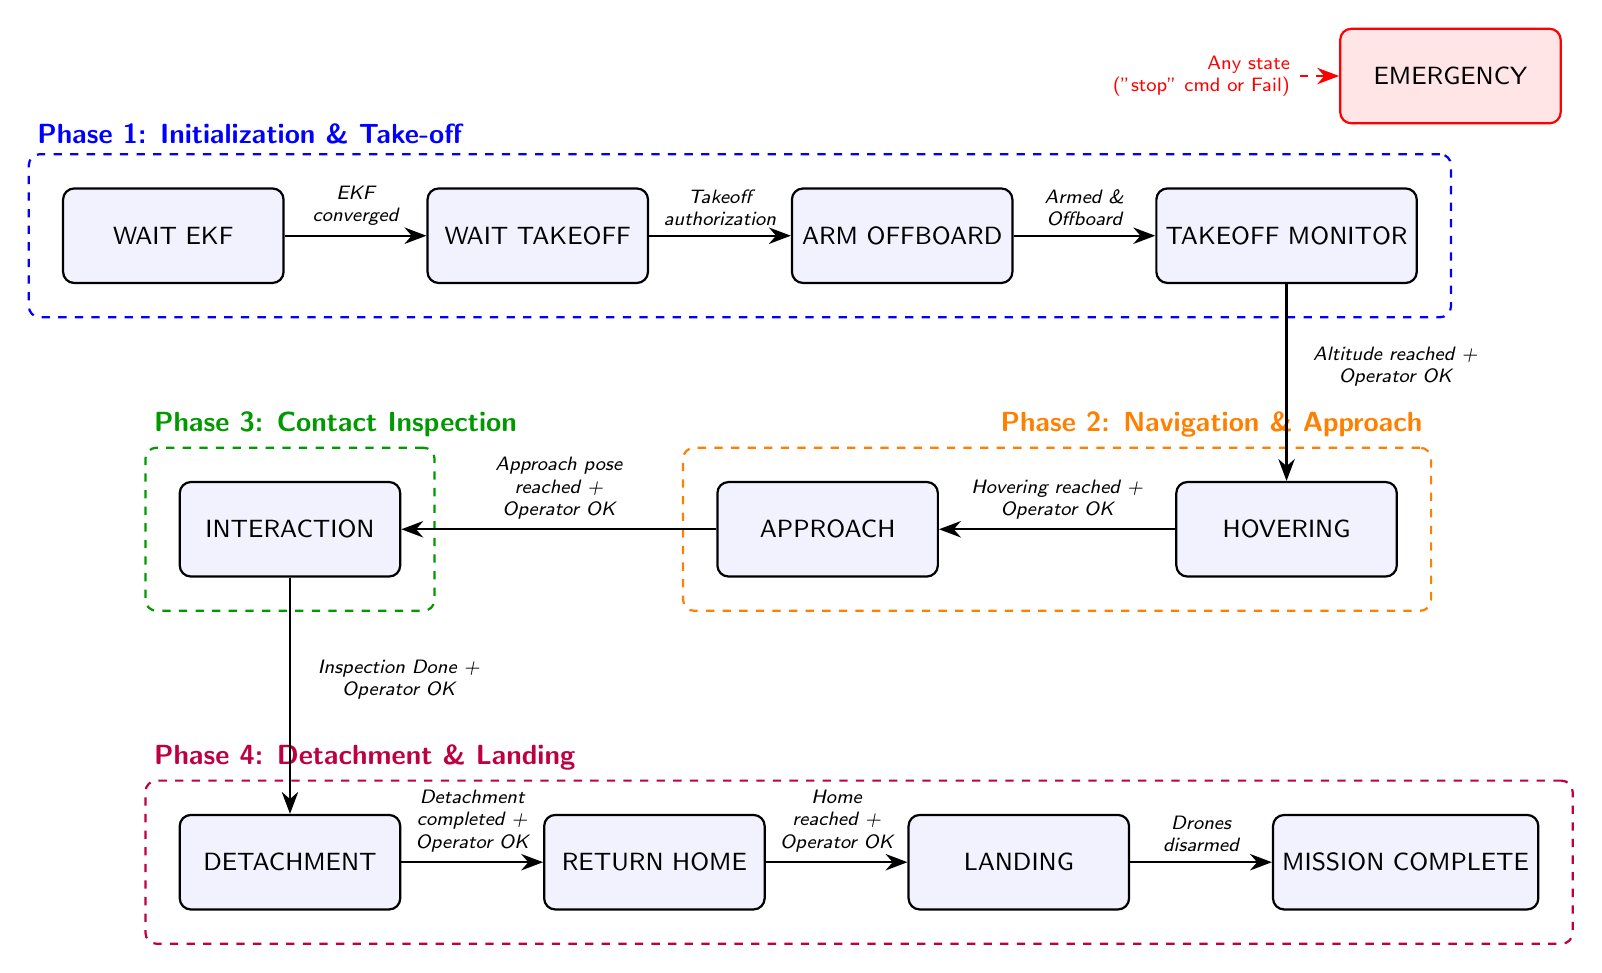
\begin{tikzpicture}[
        node distance=1.6cm and 1.8cm,
        state/.style={rectangle, rounded corners, draw=black, thick, fill=blue!5, minimum width=2.8cm, minimum height=1.2cm, text centered, font=\sffamily\small, align=center},
        arrow/.style={-{Stealth[scale=1.2]}, thick},
        phasebox/.style={rectangle, draw=#1, dashed, thick, inner sep=1.2em, rounded corners},
        labeltext/.style={font=\sffamily\scriptsize\itshape, align=center, text width=2.5cm}
    ]

    % --- ROW 1: PHASE 1 ---
    \node[state] (wait_ekf) {WAIT EKF};
    \node[state, right=of wait_ekf] (wait_takeoff) {WAIT TAKEOFF};
    \node[state, right=of wait_takeoff] (arm) {ARM OFFBOARD};
    \node[state, right=of arm] (monitor) {TAKEOFF MONITOR};

    % --- ROW 2: PHASE 2 & 3 (R-to-L flow to save space) ---
    \node[state, below=2.5cm of monitor] (hovering) {HOVERING};
    \node[state, left=3cm of hovering] (approach) {APPROACH};
    \node[state, left=4cm of approach] (interaction) {INTERACTION};

    % --- ROW 3: PHASE 4 (L-to-R flow) ---
    \node[state, below=3cm of interaction] (detachment) {DETACHMENT};
    \node[state, right=of detachment] (return_home) {RETURN HOME};
    \node[state, right=of return_home] (landing) {LANDING};
    \node[state, right=of landing] (complete) {MISSION COMPLETE};

    % --- EMERGENCY BOX ---
    \node[state, fill=red!10, draw=red, thick, above right=0.8cm and -1.0cm of monitor] (emergency) {EMERGENCY};
    \node[font=\sffamily\scriptsize\color{red}, left=0.5cm of emergency, align=right] (any) {Any state\\("stop" cmd or Fail)};
    \draw[arrow, red, dashed] (any) -- (emergency);

    % --- PHASE BACKGROUND BOXES ---
    \begin{scope}[on background layer]
        % Phase 1
        \node[phasebox=blue, fit=(wait_ekf) (monitor)] (phase1) {};
        \node[above right, font=\sffamily\bfseries\color{blue}] at (phase1.north west) {Phase 1: Initialization \& Take-off};

        % Phase 2
        \node[phasebox=orange, fit=(hovering) (approach)] (phase2) {};
        \node[above left, font=\sffamily\bfseries\color{orange}] at (phase2.north east) {Phase 2: Navigation \& Approach};

        % Phase 3
        \node[phasebox=green!60!black, fit=(interaction)] (phase3) {};
        \node[above right, font=\sffamily\bfseries\color{green!60!black}] at (phase3.north west) {Phase 3: Contact Inspection};

        % Phase 4
        \node[phasebox=purple, fit=(detachment) (complete)] (phase4) {};
        \node[above right, font=\sffamily\bfseries\color{purple}] at (phase4.north west) {Phase 4: Detachment \& Landing};
    \end{scope}

    % --- ARROWS & TRANSITIONS ---
    % Phase 1
    \draw[arrow] (wait_ekf) -- node[above, labeltext] {EKF \\converged} (wait_takeoff);
    \draw[arrow] (wait_takeoff) -- node[above, labeltext] {Takeoff\\authorization} (arm);
    \draw[arrow] (arm) -- node[above, labeltext] {Armed \&\\Offboard} (monitor);
    
    % Phase 1 -> 2
    \draw[arrow] (monitor) -- node[right, labeltext, yshift=2mm] {Altitude reached +\\Operator OK} (hovering);
    
    % Phase 2
    \draw[arrow] (hovering) -- node[above, labeltext] {Hovering reached +\\Operator OK} (approach);
    
    % Phase 2 -> 3
    \draw[arrow] (approach) -- node[above, labeltext] {Approach pose reached +\\Operator OK} (interaction);
    
    % Phase 3 -> 4
    \draw[arrow] (interaction) -- node[right, labeltext, yshift=2mm] {Inspection Done +\\Operator OK} (detachment);
    
    % Phase 4
    \draw[arrow] (detachment) -- node[above, labeltext] {Detachment completed +\\Operator OK} (return_home);
    \draw[arrow] (return_home) -- node[above, labeltext] {Home \\reached +\\Operator OK} (landing);
    \draw[arrow] (landing) -- node[above, labeltext] {Drones\\disarmed} (complete);

    \end{tikzpicture}
    } % Fine resizebox
    \caption{Finite State Machine (FSM) representing the sequential phases of the cooperative mission. State transitions are governed by autonomous checks and human-in-the-loop confirmations managed by the supervisor node.}
    \label{fig:fsm_mission}
\end{figure}

\begin{itemize}
    \item \textbf{Phase 1: Initialization and Take-off.} The mission begins with the supervisor node awaiting the full Extended Kalman Filter (EKF) convergence for both drones (\texttt{WAIT EKF}). Upon human confirmation, the system transitions to \texttt{WAIT TAKEOFF}, verifying the MPC readiness before autonomously arming and switching both vehicles to offboard control mode (\texttt{ARM OFFBOARD}). Finally, both UAVs take off and hover at a predefined safety altitude, monitored continuously until reached (\texttt{TAKEOFF MONITOR}). 
    \item \textbf{Phase 2: Navigation and Approach.} Once altitude is reached and the operator confirms, the system moves to the \texttt{HOVERING} state. The Inspection Drone (Drone 2) holds its starting coordinate, while the Camera Drone initiates the visual tracking via MPC, framing Drone 2 centrally. Following another operator confirmation, Obseerved Drone autonomously navigates towards the target inspection area (e.g., a position $2\text{ m}$ away from a bridge pillar) and aligns its yaw (\texttt{APPROACH}). Throughout this phase, Drone 1 actively maintains the target in the center of its Field of View (FOV).
    \item \textbf{Phase 3: Contact Inspection and Shared Control.} After operator confirm, the system transitions into \texttt{INTERACTION}. Drone 2 advances to make physical contact with the structure. Concurrently, the supervisor commands the MPC of Drone 1 to adopt a closer and decentered Point of View (PoV) (e.g., observing Drone 2 in the bottom-right corner of the FOV), providing optimal visual context for the task. In this phase the human operator uses haptic interface, allowing for fine-grained manual scanning.
    \item \textbf{Phase 4: Detachment and Landing.} When the inspection is concluded, an operator command triggers the \texttt{DETACHMENT} state. Drone 2 safely detaches from the wall, retreating by a predetermined distance ($1\text{ m}$), while Drone 1 widens its tracking radius to $2.0\text{ m}$, to have a larger view, while preserving the decentered PoV. Upon further clearance, the vehicles retreat to the \texttt{RETURN HOME} state: Drone 2 navigates back to its initial take-off location, and Drone 1 restores a centered PoV. Finally, the supervisor commands \texttt{LANDING}, safely bringing both drones to the ground until disarmed (\texttt{MISSION COMPLETE}). At any point during the mission, an operator ``stop" command or an offboard/arming failure triggers an immediate \texttt{EMERGENCY} state, enforcing a prompt landing.
\end{itemize}
    \chapter{Control architecture}
    This chapter goes into the detail about the mathematics used in the proposed framework, dealing with modeling, planning and optimization.
\section{Quadrotor Mathematical Model}
The aerial platforms chosen for the simulation are two planar quadcopters, one equipped with a camera rigidly mounted along its body $x$-axis and the other one with an end-effector on which a force sensor is mounted at the tip. 
\\The mathematical model can be considered as in common for both an it's a well-known quadcopter mathematical model. Let $m$ be the total mass of the drone, $\mathbf{g}=\begin{bmatrix}0 & 0 & g_0\end{bmatrix}^\top$ the gravity vector, and $\mathbf{J}=\operatorname{diag}(I_{xx},I_{yy},I_{zz})$ the diagonal inertia matrix. The 6-DoF rigid body dynamics can be expressed as follows:
\begin{equation} \label{eq:quadrotor_model}
\begin{aligned}
\dot{\mathbf{p}} &= \mathbf{v},\\
\dot{\mathbf{v}} &= \frac{1}{m}\,\mathbf{R}(\mathbf{q}) \begin{bmatrix}0\\[1mm]0\\[1mm]F_z\end{bmatrix} - \mathbf{g + \dfrac{1}{m} F_{ext}},\\
\dot{\mathbf{q}} &= \tfrac{1}{2}\,\boldsymbol{\Omega}(\boldsymbol{\omega})\,\mathbf{q}, \qquad 
\boldsymbol{\Omega}(\boldsymbol{\omega}) \!=\! \begin{bmatrix}
0 & -\omega_x & -\omega_y & -\omega_z\\
\omega_x & 0 & \omega_z & -\omega_y\\
\omega_y & -\omega_z & 0 & \omega_x\\
\omega_z & \omega_y & -\omega_x & 0
\end{bmatrix},\\
\dot{\boldsymbol{\omega}} &= \mathbf{J}^{-1}\!\left(\boldsymbol{\tau} - \boldsymbol{\omega} \times \mathbf{J}\boldsymbol{\omega}+\boldsymbol{\tau}_{ext}\right),
\end{aligned}
\end{equation}

where:
\begin{itemize}
    \item $\mathbf{p} \in \mathbb{R}^3$ is the position of the Center of Mass (CoM) in the world frame;
    \item $\mathbf{v} \in \mathbb{R}^3$ is the CoM linear velocity in the world frame;
    \item $\mathbf{q} = \begin{bmatrix} q_x & q_y & q_z & q_w \end{bmatrix}^\top$ is the unit quaternion representing the orientation of the body frame with respect to the world frame;
    \item $\boldsymbol{\omega} = \begin{bmatrix} \omega_x & \omega_y & \omega_z \end{bmatrix}^\top$ is the angular velocity expressed in the body frame;
    \item $\boldsymbol{\tau} = \begin{bmatrix} \tau_x & \tau_y & \tau_z \end{bmatrix}^\top$ and $F_z$ are the control torques and the total thrust generated by the propellers, respectively;
    \item $\mathbf{F_{ext}} \in \mathbb{R}^3$ and $\boldsymbol{\tau}_{ext} \in \mathbb{R}^3$ represent the unmodeled external forces and torques acting on the drone (e.g., aerodynamic drag, ground effect, wind, model mismatches), expressed in the world frame and body frame, respectively;
    \item $\mathbf{R}(\mathbf{q}) \in SO(3)$ is the rotation matrix from the body frame to the world frame, derived from the quaternion as:
    \begin{equation}
        \mathbf{R}(\mathbf{q}) = \begin{bmatrix}
        1-2(q_y^2+q_z^2) & 2(q_xq_y-q_zq_w) & 2(q_xq_z+q_yq_w)\\
        2(q_xq_y+q_zq_w) & 1-2(q_x^2+q_z^2) & 2(q_yq_z-q_xq_w)\\
        2(q_xq_z-q_yq_w) & 2(q_yq_z+q_xq_w) & 1-2(q_x^2+q_y^2)
        \end{bmatrix}
    \end{equation}
\end{itemize}

\section{Observer Drone: MPC-based Geometric \\Tracking}
The observer drone is designed to act as an active Point of View (PoV) for the human operator. This implies satisfying multiple simultaneous requirements: guaranteeing flight stability, maintaining the target drone within the camera's Field of View (FOV) at a desired mutual distance, ensuring a specific observation angle (e.g., frontal or lateral), and providing a smooth trajectory to minimize the operator's motion sickness. 

\subsection{From Optimal Control to MPC}
Handling multiple conflicting objectives and strict state-input constraints on an underactuated system naturally leads to the formulation of an Optimal Control Problem (OCP). In general terms, given a continuous-time dynamical system $\dot{\mathbf{x}} = f(\mathbf{x}(t), \mathbf{u}(t))$, optimal control seeks a control law $\mathbf{u}_{\text{opt}}(t)$ capable of minimizing a defined cost function $J(\mathbf{x}(t), \mathbf{u}(t))$ over a finite time horizon $T_f$. The standard continuous-time OCP can be written as:
\begin{equation}
\min_{\mathbf{x},\mathbf{u}} J(\mathbf{x}, \mathbf{u}) = \min_{\mathbf{x}, \mathbf{u}} \int_{t_0}^{t_0+T_f} L(\mathbf{x}(t), \mathbf{u}(t)) \, dt + \Phi(\mathbf{x}(t_0+T_f))
\end{equation}
\begin{center}
s.t.
$\begin{cases}
    \dot{\mathbf{x}} = f(\mathbf{x} , \mathbf{u})\\
    \mathbf{x}(t_0) = \mathbf{x}_{init}\\
    \mathbf{x}(t) \in \mathcal{X}, \mathbf{u}(t) \in \mathcal{U}
\end{cases}$
\end{center}
where $L(\mathbf{x,u})$ represents the stage cost over the horizon, and $\Phi(\mathbf{x}(t_0+T_f))$ represents the terminal cost. The system is subject to the continuous dynamics(eq. \ref{eq:quadrotor_model}), initial conditions, and feasible sets for states and inputs.
\\Solving a standard OCP yields an open-loop trajectory, which is inadequate for the proposed shared-control architecture. The target drone moves dynamically, and the human operator can unpredictably alter its trajectory. Therefore, an online, closed-loop planner is required. This is achieved through Model Predictive Control (MPC).
\\To transition from the continuous-time formulation to a tractable numerical problem, the system dynamics are discretized using an Explicit Runge-Kutta (ERK) integrator. The MPC algorithm solves the resulting discrete-time OCP over a receding prediction horizon of $N$ steps at each sampling time $T_s$, generating an optimal control sequence from which only the first element is applied to the plant. This process constantly updates the initial conditions based on state feedback, providing real-time tracking, robustness against model uncertainties, and the ability to incorporate the human operator's inputs.

\subsection{NMPC Problem Formulation}
\subsubsection{Nonlinear Least Square Cost Function}
In formulating the OCP, we first define the vectors of the cost terms that need to be optimized over the prediction horizon. The stage cost vector $\mathbf{y}_k$ and the terminal cost vector $\mathbf{y}_N$ are composed of the actual system states and control inputs:
\begin{align}
    \mathbf{y}_k &= \begin{bmatrix} \mathbf{p}^T, \psi, \mathbf{v}^T, \boldsymbol{\omega}^T, \dot{\mathbf{v}}^T, \dot{\boldsymbol{\omega}}^T, \ddot{\mathbf{v}}^T, \dddot{\mathbf{v}}^T, \mathbf{u}^T \end{bmatrix}^T, \\
    \mathbf{y}_N &= \begin{bmatrix} \mathbf{p}^T, \psi, \mathbf{v}^T, \boldsymbol{\omega}^T, \dot{\mathbf{v}}_{\text{hov}}^T, \dot{\boldsymbol{\omega}}_{\text{hov}}^T, \ddot{\mathbf{v}}_{\text{hov}}^T, \dddot{\mathbf{v}}_{\text{hov}}^T \end{bmatrix}^T.
\end{align}
In this formulation, $\mathbf{p}$ is the absolute Cartesian position of the drone and $\psi$ is its actual yaw angle. The vectors $\dot{\mathbf{v}}, \ddot{\mathbf{v}}, \dddot{\mathbf{v}}$ and $\dot{\boldsymbol{\omega}}$ denote linear acceleration, jerk, snap, and angular acceleration, which are penalized to minimize the operator's motion sickness.
\\To evaluate the tracking performance, these actual terms must be compared with a reference vector $\mathbf{y}_{\text{ref},k}$. As previously stated, bringing cylindrical transformations directly into the cost evaluation introduces non-linearities and variable Jacobians. To maintain a well-conditioned numerical problem, the desired cylindrical references $(r_{ref}, \beta_{ref}, z_{rel,ref})$ are mapped externally into an absolute cartesian target position $\mathbf{p}_{\text{ref}} = [x_{\text{ref}}, y_{\text{ref}}, z_{\text{ref}}]^\top$. By inverting Eq. (\ref{eq:cyl_mapping}), this external mapping is computed as:
\begin{align}
    x_{\text{ref}} &= x_{\text{obj}} + r_{ref} \cos(\beta_{ref}), \\
    y_{\text{ref}} &= y_{\text{obj}} + r_{ref} \sin(\beta_{ref}), \\
    z_{\text{ref}} &= z_{\text{obj}} + z_{rel,ref}.
\end{align}
With the position references mapped into the absolute world frame, the complete reference vector $\mathbf{y}_{\text{ref},k}$ is assembled using $\mathbf{p}_{\text{ref}}$ and the desired yaw $\psi_{ref}$. The objective of the nonlinear MPC is then formulated as a discrete-time Nonlinear Least Squares (NLS) optimization problem, which minimizes the tracking error between the cost vectors and the reference vectors over the horizon $N$:
\begin{equation}
    \min_{\mathbf{u}, \mathbf{x}} \sum_{k=0}^{N-1} \left( \|\mathbf{y}_k - \mathbf{y}_{\text{ref},k}\|_{\mathbf{W}}^2 \right) + \|\mathbf{y}_N - \mathbf{y}_{\text{ref},N}\|_{\mathbf{W}_e}^2,
\end{equation}
where $\mathbf{W}$ and $\mathbf{W}_e$ are the diagonal weight matrices for the stage and terminal costs, respectively. By decoupling the geometrical transformations from the objective function, this strategy guarantees that the positional error tracking maintains a constant identity Jacobian, thereby improving solver stability and execution speed.
\subsubsection{Weight matrices}
Given the heterogeneous quantities in the residual vector $\mathbf{y}_k$, an unscaled weight matrix leads to numerical ill-conditioning. The diagonal weight matrices $\mathbf{W} = \operatorname{blkdiag}(\mathbf{Q}, \mathbf{R})$ and $\mathbf{W}_e$ are constructed using Bryson's rule normalization~\cite{bryson1975applied}. Each diagonal element is scaled inversely proportional to the square of its maximum expected deviation:
\begin{equation}
    W_{ii} = \frac{w_i}{(\Delta y_{i, \max})^2}
\end{equation}
where $w_i$ is the relative priority weight of the specific objective and $\Delta y_{i, \max}$ is the maximum acceptable tolerance for that state. This normalization prevents higher-order physical limits from dominating the geometric framing requirements. The terminal weight matrix $\mathbf{W}_e$ follows a similar structure, lacking the input partition $\mathbf{R}$.

\subsubsection{Constraints}
A first constraint set of te OCP is given by the system dynamics:
\begin{align}
    \mathbf{x}_{k+1} &= \mathbf{f}_d(\mathbf{x}_k, \mathbf{u}_k), \\
    \mathbf{x}_0 &= \bar{\mathbf{x}}_{\text{init}},
\end{align}
where $\mathbf{f}_d$ represents the explicit Runge-Kutta discretization of the quadrotor model represented by ~\ref{eq:quadrotor_model}. Actuation and workspace limitations are enforced via hard box constraints on the control inputs $\mathbf{u}_k = [F_z, \tau_x, \tau_y, \tau_z]^\top$:
\begin{equation}
    \begin{bmatrix} 0 \\ -U_{\tau x} \\ -U_{\tau y} \\ -U_{\tau z} \end{bmatrix} \le 
    \mathbf{u}_k \le 
    \begin{bmatrix} U_F \\ U_{\tau x} \\ U_{\tau y} \\ U_{\tau z} \end{bmatrix}.
\end{equation}
While maintaining the target in the Field of View (FOV) could be treated via explicit inequality soft-constraints, the chosen approach was to handle these constraints only with haptic feedback. Therefore, visual and safety requirements are induced through the weighted and normalized tracking cost, coupled with the external Artificial Potential Fields (APF) (see \ref{section:APF}) acting on the human input. This keeps the reference fed to the MPC within the optical frustum limits, allowing the solver to focus purely on dynamically feasible and smooth trajectory generation.
\begin{figure}[htbp]
\centering
\resizebox{\textwidth}{!}{%
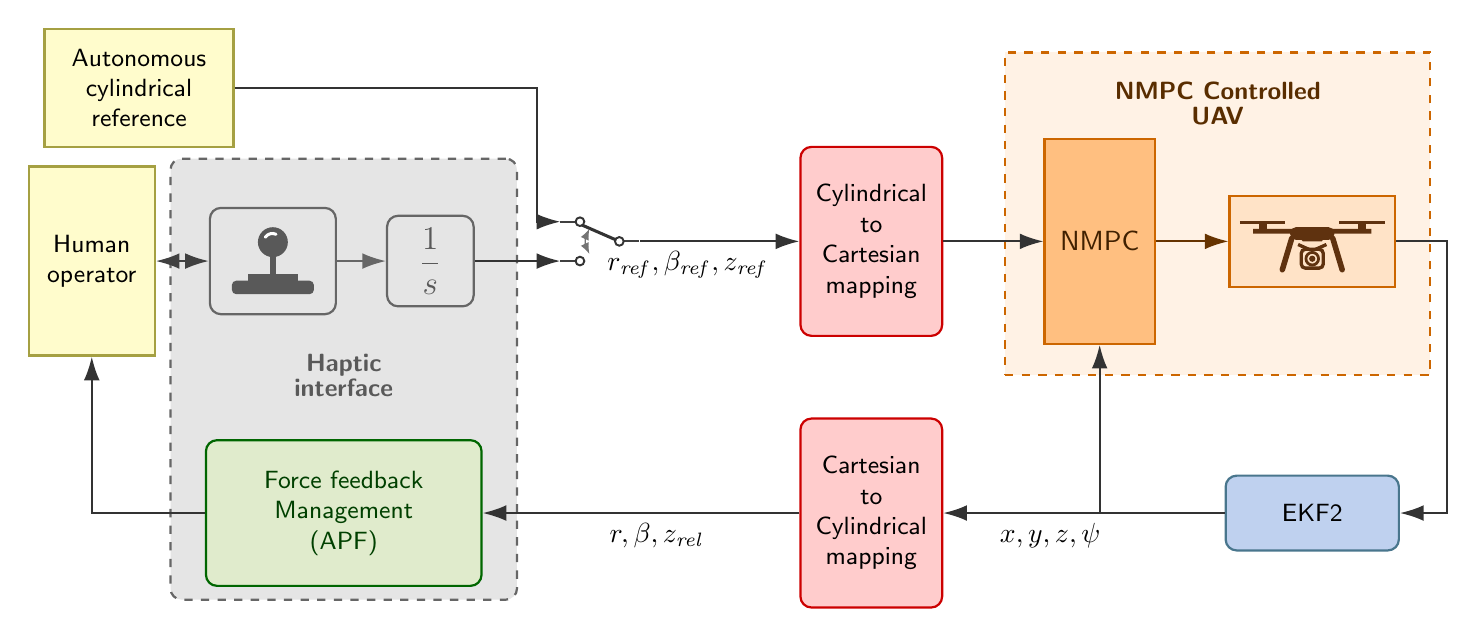
\begin{tikzpicture}[
    font=\sffamily\small,
    >= {Latex[length=3mm, width=2mm]},
    % Definizione colori 
    colYellow/.style={fill=yellow!20!, draw=yellow!60!black, thick},
    colHapticBg/.style={fill=black!10!, draw=gray!80!black, dashed, thick},
    colInnerGray/.style={fill=black!10!, draw=gray!80!black, thick},
    colSwitch/.style={fill=black!0, draw=white!80, thick},
    colGreen/.style={fill=green!20!olive!20!, draw=green!40!black, thick},
    colMap/.style={fill=red!20!, draw=red!80!black!, thick},
    colUavBg/.style={fill=orange!10!, draw=orange!80!black, dashed, thick},
    colNmpc/.style={fill=orange!50!, draw=orange!80!black, thick},
    colDroneBox/.style={fill=orange!22, draw=orange!80!black, thick},
    colEkf/.style={fill=cyan!55!blue!25, draw=cyan!50!black, thick},
    % Stile linee di connessione
    conn/.style={->, draw=black!80, line width=0.7pt},
    connGray/.style={->, draw=black!60, line width=0.7pt},
    % =========================================================
    % ICONA 1: Joystick / Haptic (Disegnata nativamente in TikZ)
    % =========================================================
    joystick/.pic={
        % Base inferiore
        \fill[black!65, rounded corners=1.5pt] (-0.52,-0.42) rectangle (0.52,-0.25);
        % Gradino superiore base
        \fill[black!65] (-0.32,-0.25) rectangle (0.32,-0.16);
        % Asta
        \draw[black!65, line width=2.4pt] (0,-0.16) -- (0,0.18);
        % Sfera (Pomello)
        \fill[black!65] (0,0.24) circle (0.19);
        % Riflesso bianco sulla sfera
        \draw[white, line width=1.1pt, line cap=round] (0.04,0.34) arc (65:145:0.11);
    },
    % =========================================================
    % ICONA 2: Quadrotore con Camera (Disegnata nativamente)
    % =========================================================
    quadrotor/.pic={
        \definecolor{dronebr}{RGB}{95, 50, 15}
        % Bracci e corpo centrale
        \fill[dronebr] (-0.75, 0.10) -- (-0.20, 0.10) -- (-0.12, 0.0) -- (0.12, 0.0) -- (0.20, 0.10) -- (0.75, 0.10) -- (0.75, 0.16) -- (-0.75, 0.16) -- cycle;
        \fill[dronebr, rounded corners=2pt] (-0.28, 0.02) rectangle (0.28, 0.18);
        % Motori ed eliche
        \fill[dronebr] (-0.68, 0.16) rectangle (-0.58, 0.24);
        \fill[dronebr] (0.58, 0.16) rectangle (0.68, 0.24);
        \draw[dronebr, line width=1.4pt] (-0.92, 0.24) -- (-0.34, 0.24);
        \draw[dronebr, line width=1.4pt] (0.34, 0.24) -- (0.92, 0.24);
        % Carrelli di atterraggio
        \draw[dronebr, line width=2pt, line cap=round] (-0.26, 0.04) -- (-0.38, -0.36);
        \draw[dronebr, line width=2pt, line cap=round] (0.26, 0.04) -- (0.38, -0.36);
        % Supporto e Telecamera centrale
        \draw[dronebr, line width=1.2pt] (-0.18, -0.04) -- (0, -0.12) -- (0.18, -0.04);
        \draw[dronebr, fill=orange!22, line width=1.2pt, rounded corners=1.5pt] (-0.14, -0.34) rectangle (0.14, -0.10);
        \draw[dronebr, line width=1pt] (0, -0.22) circle (0.08);
        \fill[dronebr] (0, -0.22) circle (0.04);
    }
]

    % ---------------------------------------------------------
    % 1. CONTENITORI TRATTEGGIATI DI SFONDO
    % ---------------------------------------------------------
    % Contenitore Haptic Interface
    \node[colHapticBg, minimum width=4.4cm, minimum height=5.6cm, rounded corners] (haptic_bg) at (3.6, -1.5) {};
    \node[text=black!65, align=center, rounded corners] at (3.6, -1.45) {\textbf{Haptic}\\[-2pt]\textbf{interface}};

    % Contenitore NMPC Controlled UAV
    \node[colUavBg, minimum width=5.4cm, minimum height=4.1cm] (uav_bg) at (14.7, 0.60) {};
    \node[text=orange!35!black, align=center] at (14.7, 2.00) {\textbf{NMPC Controlled}\\[-2pt]\textbf{UAV}};

    % ---------------------------------------------------------
    % 2. BLOCCHI PRINCIPALI
    % ---------------------------------------------------------
    % Colonna Sinistra: Riferimento autonomo e Operatore Umano
    \node[colYellow, minimum width=2.4cm, minimum height=1.5cm, align=center] (auto_ref) at (1.0, 2.2) {Autonomous\\cylindrical\\reference};
    
    \node[colYellow, minimum width=1.6cm, minimum height=2.4cm, align=center] (human) at (0.4, 0.0) {Human\\operator};

    % Blocchi interni a Haptic Interface
    \node[colInnerGray, minimum width=1.6cm, minimum height=1.35cm, rounded corners] (joy_box) at (2.7, 0.0) {};
    \pic at (joy_box.center) {joystick};

    \node[colInnerGray, minimum width=1.1cm, minimum height=1.15cm, font=\large, text=black!65, rounded corners] (integrator) at (4.7, 0.0) {$\dfrac{1}{s}$};

    \node[colGreen, minimum width=3.5cm, minimum height=1.85cm, align=center, text=green!25!black, rounded corners] (apf) at (3.6, -3.2) {Force feedback\\Management\\(APF)};

    % ---------------------------------------------------------
    % BLOCCO SWITCH (Selettore Riferimento Autonomo / Aptico)
    % ---------------------------------------------------------
    \node[colSwitch, minimum width=1.0cm, minimum height=1.15cm] (switch_box) at (6.85, 0.25) {};
    % Tratti interni di collegamento ai terminali
    \draw[black!75, line width=0.7pt] (6.35, 0.50) -- (6.58, 0.50);
    \draw[black!75, line width=0.7pt] (6.35, 0.00) -- (6.58, 0.00);
    \draw[black!75, line width=0.7pt] (7.12, 0.25) -- (7.35, 0.25);
    % Leva interna dello switch e freccia di commutazione
    \draw[black!80, line width=1.1pt, line cap=round] (7.10, 0.25) -- (6.62, 0.46);
    \draw[<->, >={Latex[length=1.4mm, width=1.1mm]}, black!55, line width=0.45pt] (6.72, 0.41) to[bend right=25] (6.72, 0.09);
    % Terminali (pallini bianchi)
    \filldraw[fill=white, draw=black!80, line width=0.7pt] (6.60, 0.50) circle (0.055);
    \filldraw[fill=white, draw=black!80, line width=0.7pt] (6.60, 0.00) circle (0.055);
    \filldraw[fill=white, draw=black!80, line width=0.7pt] (7.10, 0.25) circle (0.055);

    % Colonna Centrale: Blocchi di Mapping
    \node[colMap, minimum width=1.8cm, minimum height=2.4cm, align=center, rounded corners] (cyl2cart) at (10.3, 0.25) {Cylindrical\\to\\Cartesian\\mapping};

    \node[colMap, minimum width=1.8cm, minimum height=2.4cm, align=center, rounded corners] (cart2cyl) at (10.3, -3.2) {Cartesian\\to\\Cylindrical\\mapping};

    % Blocchi interni a NMPC Controlled UAV
    \node[colNmpc, minimum width=1.4cm, minimum height=2.6cm, align=center, text=orange!25!black, font=\sffamily\bfseriesm] (nmpc) at (13.2, 0.25) {NMPC};

    \node[colDroneBox, minimum width=2.1cm, minimum height=1.15cm] (drone_box) at (15.9, 0.25) {};
    \pic at (drone_box.center) {quadrotor};

    % Blocco EKF2 in basso a destra
    \node[colEkf, minimum width=2.2cm, minimum height=0.95cm, align=center, rounded corners] (ekf) at (15.9, -3.2) {EKF2};

    % ---------------------------------------------------------
    % 3. FRECCE E COLLEGAMENTI
    % ---------------------------------------------------------
    % Interazione bidirezionale Human <-> Joystick
    \draw[<->, draw=black!75, line width=0.7pt] (human.east) -- (joy_box.west);

    % Joystick -> 1/s
    \draw[connGray] (joy_box.east) -- (integrator.west);

    % 1/s -> Ingresso inferiore dello Switch
    \draw[conn] (integrator.east) -- (6.35, 0.00);

    % Autonomous cylindrical reference -> Ingresso superiore dello Switch
    \draw[conn] (auto_ref.east) -| (6.05, 0.50) -- (6.35, 0.50);

    % Uscita Switch -> Cylindrical to Cartesian mapping
    \draw[conn] (switch_box.east) -- node[below, pos=0.3, font=\normalsize, text=black] {$r_{\mathit{ref}}, \beta_{\mathit{ref}}, z_{\mathit{ref}}$} (cyl2cart.west);

    % Cylindrical to Cartesian mapping -> NMPC
    \draw[conn] (cyl2cart.east) -- (nmpc.west);

    % NMPC -> Drone
    \draw[->, draw=orange!40!black, line width=0.7pt] (nmpc.east) -- (drone_box.west);

    % Drone -> EKF2 (anello esterno a destra)
    \draw[conn] (drone_box.east) -- ++(0.65, 0) |- (ekf.east);

    % EKF2 -> Cartesian to Cylindrical mapping
    \draw[conn] (ekf.west) -- node[below, pos=0.62, font=\normalsize, text=black] {$x, y, z, \psi$} (cart2cyl.east);

    % Diramazione da uscita EKF2 verso il basso di NMPC
    \coordinate (ekf_branch) at (13.2, -3.2);
    \draw[conn] (ekf_branch) -- (nmpc.south);

    % Cartesian to Cylindrical mapping -> APF
    \draw[conn] (cart2cyl.west) -- node[below, pos=0.45, font=\normalsize, text=black] {$r, \beta, z_{\mathit{rel}}$} (apf.east);

    % APF -> Human operator
    \draw[conn] (apf.west) -| (human.south);

\end{tikzpicture}%
}
\caption{NMPC Shared Control architecture.}
\label{fig:nmpc_shared_control_tikz}
\end{figure}

\subsection{Momentum-Based Wrench Estimator}
Standard optimal controllers rely on a nominal dynamic model. In real flight conditions, however, a UAV is constantly subject to unmodeled external disturbances such as aerodynamic drag, ground effect, payload shifts, or ambient wind. If neglected, these disturbances introduce either instability or steady-state tracking offsets and degrade visual framing. To counteract these effects without requiring dedicated onboard force/torque sensors, the control architecture is augmented with a Momentum-Based Estimator (MBE)~\cite{ruggiero2015passivity}. This observer estimates the unmodeled external wrench purely by tracking the discrepancy between the expected and actual generalized momentum of the vehicle, which is defined as
\begin{equation}
\begin{cases}
    \mathbf{p}_T=m\mathbf{v}\\
    \boldsymbol{\tau}_R=J\boldsymbol{\omega}
\end{cases}
\end{equation} 
\\The estimated external wrench $(\hat{\mathbf{F}}_{ext}, \hat{\boldsymbol{\tau}}_{ext})$ is evaluated online at each control step ($100\text{ Hz}$) and used directly into the NMPC solver as an online parameter vector. 
Rather than waiting for trajectory deviations to occur and reacting through feedback error, the NMPC embeds these estimated disturbances directly into its predictive model. This generates an anticipatory feedforward action that counteracts external forces and aerodynamic torques in real time, effectively eliminating steady-state position errors and maintaining high visual tracking accuracy.
For more mathematical details see \ref{app:implementation_details}.

\section{Inspection Drone: Admittance Control for Contact}
While the observer drone relies on an optimization-based framework to handle visual constraints, the inspection drone operates under a completely different control paradigm, made for physical interaction. Its primary objective is to transition safely from free flight to a stable contact state against a rigid structure. To achieve this, the control architecture is built upon a cascaded structure: a high-level planner generates the nominal motion, while an admittance filter dynamically adjusts this reference based on environmental feedback, ultimately feeding a compliant setpoint to the native PX4 position controller.
\begin{figure}[h!]
    \centering
    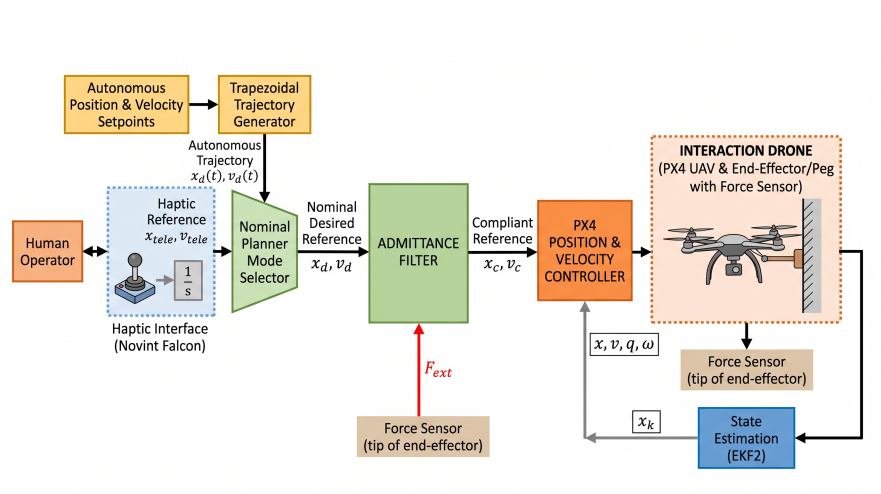
\includegraphics[width=\linewidth]{Immagini/Capitolo4/INTERACTION_DRONE_scheme.png}
    \caption{Planning and control scheme describing Interaction UAV architecture}
    \label{fig:placeholder}
\end{figure}
\subsection{High-Level Planner}
The high-level planner is responsible for generating a nominal Cartesian trajectory, denoted as $\mathbf{x}_d(t)$, which guides the inspection drone from its initial hovering state to the target surface. This reference trajectory dictates the desired 3D position and heading over time, ensuring a smooth and bounded approach velocity. However, this planned path is purely kinematic and geometric; it assumes a free-space environment and does not account for the reaction forces that arise upon impact. During the free-flight phase, the underlying flight controller tracks $\mathbf{x}_d(t)$ precisely. Yet, if the drone were to persistently track this rigid setpoint after establishing contact with the wall, the spring force by positional error action of the position controller united with integral action would rapidly accumulate error, leading to actuator saturation, violent rebounds, and inevitable instability.

\subsection{Admittance Filter}
To safely manage the transition and maintain a stable physical interaction, an admittance control strategy is implemented. This framework renders the drone compliant to external forces by masking the rigid structure as a virtual mass-spring-damper system. The core of the admittance filter~\cite{siciliano2008springer} is governed by the following second-order differential equation:
\begin{equation}
    \mathbf{M}_d \ddot{\mathbf{e}} + \mathbf{D}_d \dot{\mathbf{e}} + \mathbf{K}_d \mathbf{e} = \mathbf{F}_{ext}
\end{equation}
where $\mathbf{e}(t) = \mathbf{x}_c(t) - \mathbf{x}_d(t)$ represents the positional deviation between the newly generated compliant reference $\mathbf{x}_c(t)$ and the nominal planner trajectory $\mathbf{x}_d(t)$. The matrices $\mathbf{M}_d$, $\mathbf{D}_d$, and $\mathbf{K}_d$ are positive-definite diagonal matrices representing the desired virtual mass, damping, and stiffness, respectively. The vector $\mathbf{F}_{ext}$ represents the external contact force measured by the end-effector's onboard force sensor.
\\By numerically integrating this dynamic equation in real time, the filter evaluates the necessary spatial deviation and outputs the compliant setpoint $\mathbf{x}_c(t)$. The behavior of the system is thus completely shaped by the chosen virtual parameters. During free flight, since the measured external force is zero ($\mathbf{F}_{ext} = \mathbf{0}$), the positional error $\mathbf{e}(t)$ converges to zero, and the compliant reference matches the nominal one ($\mathbf{x}_c = \mathbf{x}_d$). Upon impact, the reaction force $\mathbf{F}_{ext}$ drives the admittance dynamics, causing the compliant reference to yield backward. This dynamically adjusted setpoint $\mathbf{x}_c(t)$ is continuously fed to the standard PX4 cascaded PID controller. As a result, the drone safely absorbs the impact and maintains a steady pressure against the surface, achieving the desired contact force without destabilizing the flight dynamics.

%%%%%%%%%%%%%%%%%%%%%%%% SHARED CONTROL %%%%%%%%%%%%%%%%%%%%%%%%%%%%%

\section{Human-Robot Shared Control}
\subsection{Teleoperation Modalities}
The proposed shared autonomy architecture allows the human operator to intervene in the mission through a haptic interface.
\begin{figure}[h!]
    \centering
    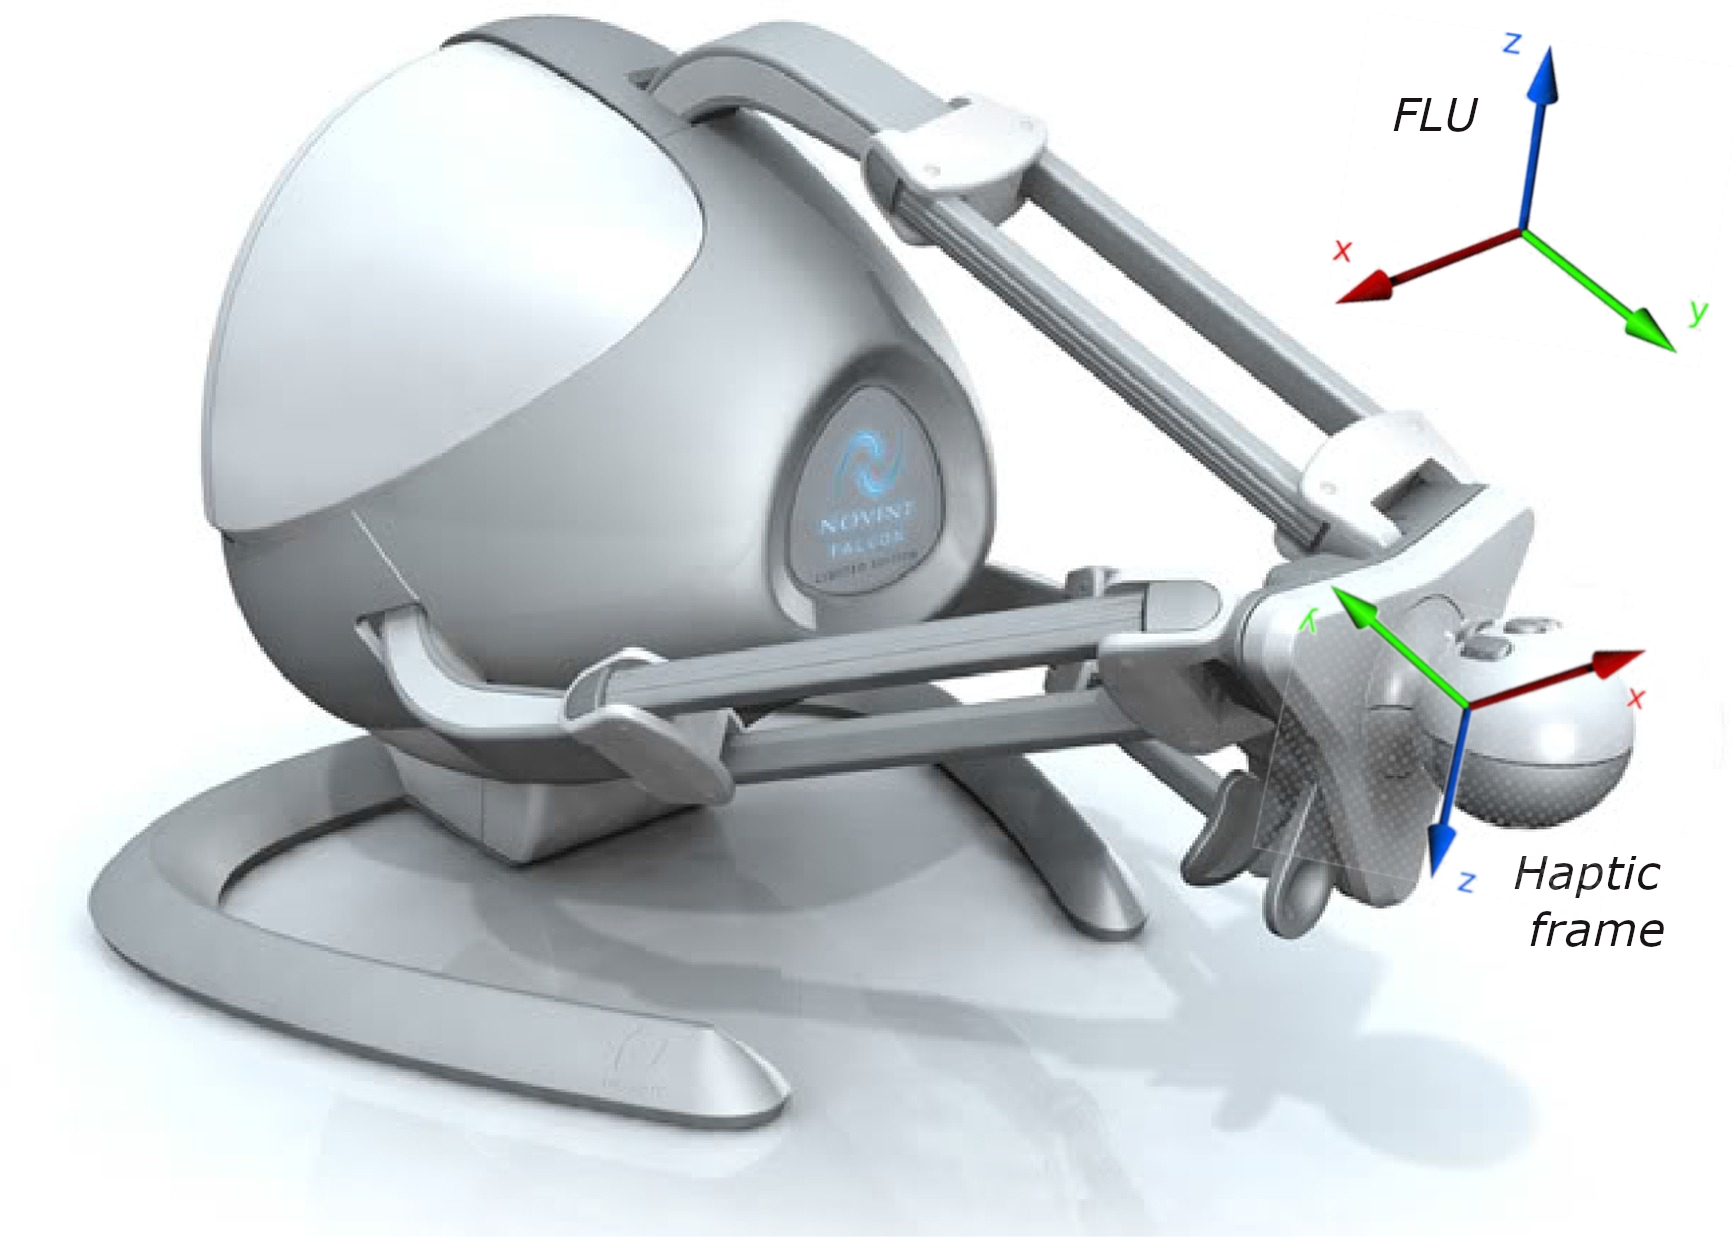
\includegraphics[width=0.5\linewidth]{Immagini/Capitolo4/Falcon_render.jpg}
    \caption{Haptic Interface Novint Falcon, used in simulations and experiments}
    \label{fig:placeholder}
\end{figure}
Depending on the operational phase and the specific mission requirements, the user can interact with the robotic team using two distinct teleoperation modalities:
\begin{itemize}
    \item \textbf{Observer Drone Control Mode:} The operator dynamically adjusts the Point of View of the camera drone. By manipulating the haptic device, the user modifies the relative distance, relative height, and azimuth angle around the inspection target. This mode enhances situational awareness and allows the operator to inspect specific structural details without disrupting the autonomous tracking.
    \item \textbf{Interaction Drone Control Mode:} During the critical phase of physical interaction, the operator can take direct control of the inspection drone to guide the fine insertion maneuver. In this phase, the human's cognitive judgment and dexterity are coupled with the autonomous admittance filter, which guarantees physical stability upon contact with the environment.
\end{itemize}

\subsection{Reference Generation via Haptic}
The used device, Novint Falcon, provides a physical 3D workspace of approximately $10 \times 10 \times 10$ cm, offering three translational degrees of freedom.  To mitigate the effects of sensor noise and unintentional operator tremors within this confined workspace, a nonlinear deadband with a threshold $d$ is applied to the raw input:
\begin{equation}
    f_{\text{db}}(x, d) = 
    \begin{cases} 
      0 & \text{if } |x| < d \\
      x - \operatorname{sgn}(x)d & \text{if } |x| \geq d
   \end{cases},
\end{equation}
\begin{figure}[h!]
    \centering
    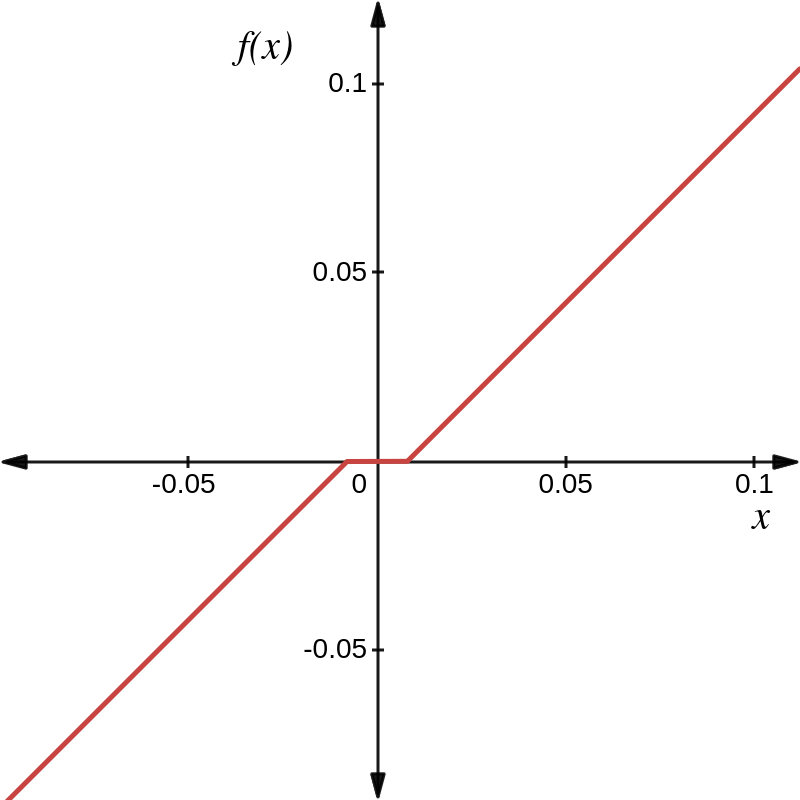
\includegraphics[width=0.5\linewidth]{Immagini/Capitolo4/Nonlinear_deadband_force.png}
    \caption{Nonlinear deadband applied on force given by the user on haptic device, $d=0.008$}
    \label{fig:haptic_render}
\end{figure}
where in this case $x\in[-0.1,0.1]$ m is a generic haptic end-effector coordinate in haptic frame (\ref{fig:haptic_render})(see Appendix \ref{app:implementation_details}). When operating in the observer control mode, the haptic interface is utilized to dynamically command the 3D reference for the camera drone in cylindrical coordinates[\ref{eq:cyl_mapping}]: this provides a human intuitive commanding modality for a target tracking, in relation to what he sees and which movements he can really perform with an underactuated drone (i.e, it would be useless to use spherical coordinates for 4 DOF UAV).  
In order to maintain consistency with the OCP formulation, the displacements of the haptic end-effector are directly mapped into reference velocities for the cylindrical variables. Specifically, the $x_h$, $y_h$, and $z_h$ inputs govern the rate of change of the radial distance $\dot{r}_{cyl}$, the azimuth orbit $\dot{\beta}$, and the relative altitude $\dot{z}_{rel}$, respectively. The position of device's end-effector in this operational space is denoted as $\mathbf{p}_h = [x_h, y_h, z_h]^\top$ and there is, clearly, the necessity to translate such small movements in bigger ones for feeding the drone with a proper reference. By introducing a generic scaling factor $K_{\text{joy}}=15$, the reference velocities imposed by the user are defined as:
\begin{equation}
    \begin{bmatrix} \dot{r}_{cyl} \\ \dot{\beta} \\ \dot{z}_{rel} \end{bmatrix} = 
    K_{\text{joy}} \begin{bmatrix} 
    v_{r,\max} \cdot f_{\text{db}}(x_h, d) \\ 
    v_{\beta,\max} \cdot f_{\text{db}}(y_h, d) \\ 
    v_{z,\max} \cdot f_{\text{db}}(z_h, d) 
    \end{bmatrix}
\end{equation}
These velocities are numerically integrated over the control loop time step $\Delta t$ to generate the desired cylindrical reference vector. To avoid kinematic singularities and physically unfeasible setpoints, bounds are applied during the integration step: the radial distance is strictly kept above a minimum safety threshold (avoiding singularity in $r=0$), and the azimuth angle is wrapped within the $[-\pi, \pi]$ interval to ensure continuity in rotation. The resulting updated reference vector $\mathbf{y}_{\text{ref}}(t) = [r_{cyl,\text{ref}}, \beta_{\text{ref}}, z_{rel,\text{ref}}]^\top$ is then published to the MPC planner, dynamically shifting the optimal tracking objective.

\subsection{Force Feedback Management}
\label{section:APF}
Force feedback has been handled with a sum of two contribution given back to the user.
\\A base mechanical impedance is applied to provide the user with a tactile sensation of stability and centering with respect to the origin (i.e., zero imposed velocity). This behavior is modeled as a virtual spring-damper system:
\begin{equation}
    \mathbf{F}_{\text{imp}} = -k \cdot \mathbf{p}_h - b \cdot \dot{\mathbf{p}}_h
\end{equation}
In addition to this base impedance, to ensure the safety of the visual tracking maneuver and prevent the observer drone from losing sight of the target or getting too close to it, a haptic force feedback based on Artificial Potential Fields is also rendered to the operator. This feedback translates undesired behaviors for the drone into a physical sensation for the human.
\\To do this, we need to mathematically define the physical boundaries of the camera's optical frustum and the drone's safety area. These boundaries impose spatial constraints that are continuously compared with the actual measured state $\mathbf{y}_{\text{act}} = [r_{\text{act}}, \beta_{\text{act}}, z_{\text{act}}, \psi_{\text{dev}}]^\top$, where $\psi_{\text{dev}}$ is the yaw deviation of the target from the camera's optical center.
\\First, let us define the vertical physical limit of the camera's vision. From a top-down perspective, if the target is at a radial distance $r_{\text{act}}$, its projected depth along the camera's optical axis is $r_{\text{act}} \cos(\psi_{\text{dev}})$. Using basic trigonometry on the vertical plane, the maximum visible height from the center of the image to the top or bottom edge is defined as:
\begin{equation}
    z_{\max} = r \cos(\psi_{\text{dev}}) \tan\left(\frac{\text{FOV}_v}{2}\right)
\end{equation}
\begin{figure}[htbp]
    \centering
    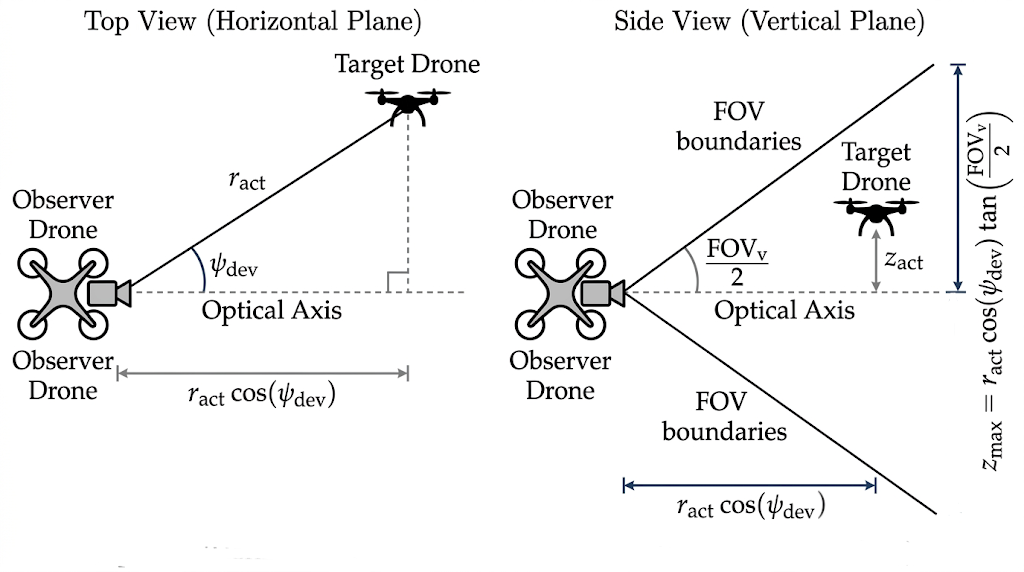
\includegraphics[width=\linewidth]{Immagini/Capitolo4/FOV_boundaries.png}
    \caption{Top and side views of the two drones}
    \label{fig:placeholder}
\end{figure}
\justify
where $FOV_v$ is a parameter denoting the maximum vertical optical aperture of the camera. 
\\\textbf{Notice}: this is an approximation. This supposes the camera optical axes to be always parallel to world XY plane (i.e., flat drone). Since camera is rigidly mounted on Observer Drone body frame, UAV must roll and pitch in order to move. This could be avoided by bringing distance in Observer UAV's body frame, but it's acceptable for smooth desired motion.
\\Using $z_{\max}$, we can easily define the distances from the actual drone state to the boundaries of the image. These spatial margins are geometrically defined as follows:
\begin{align}
    \Delta r &= r_{\text{act}} - r_{\min} \\
    \Delta z_{\text{top}} &= z_{\max} - z_{\text{act}} \\
    \Delta z_{\text{bot}} &= z_{\text{act}} + z_{\max} \\
    \Delta \psi &= \frac{\text{FOV}_h}{2} - |\psi_{\text{dev}}|
\end{align}
\begin{figure}[h!]
    \centering
    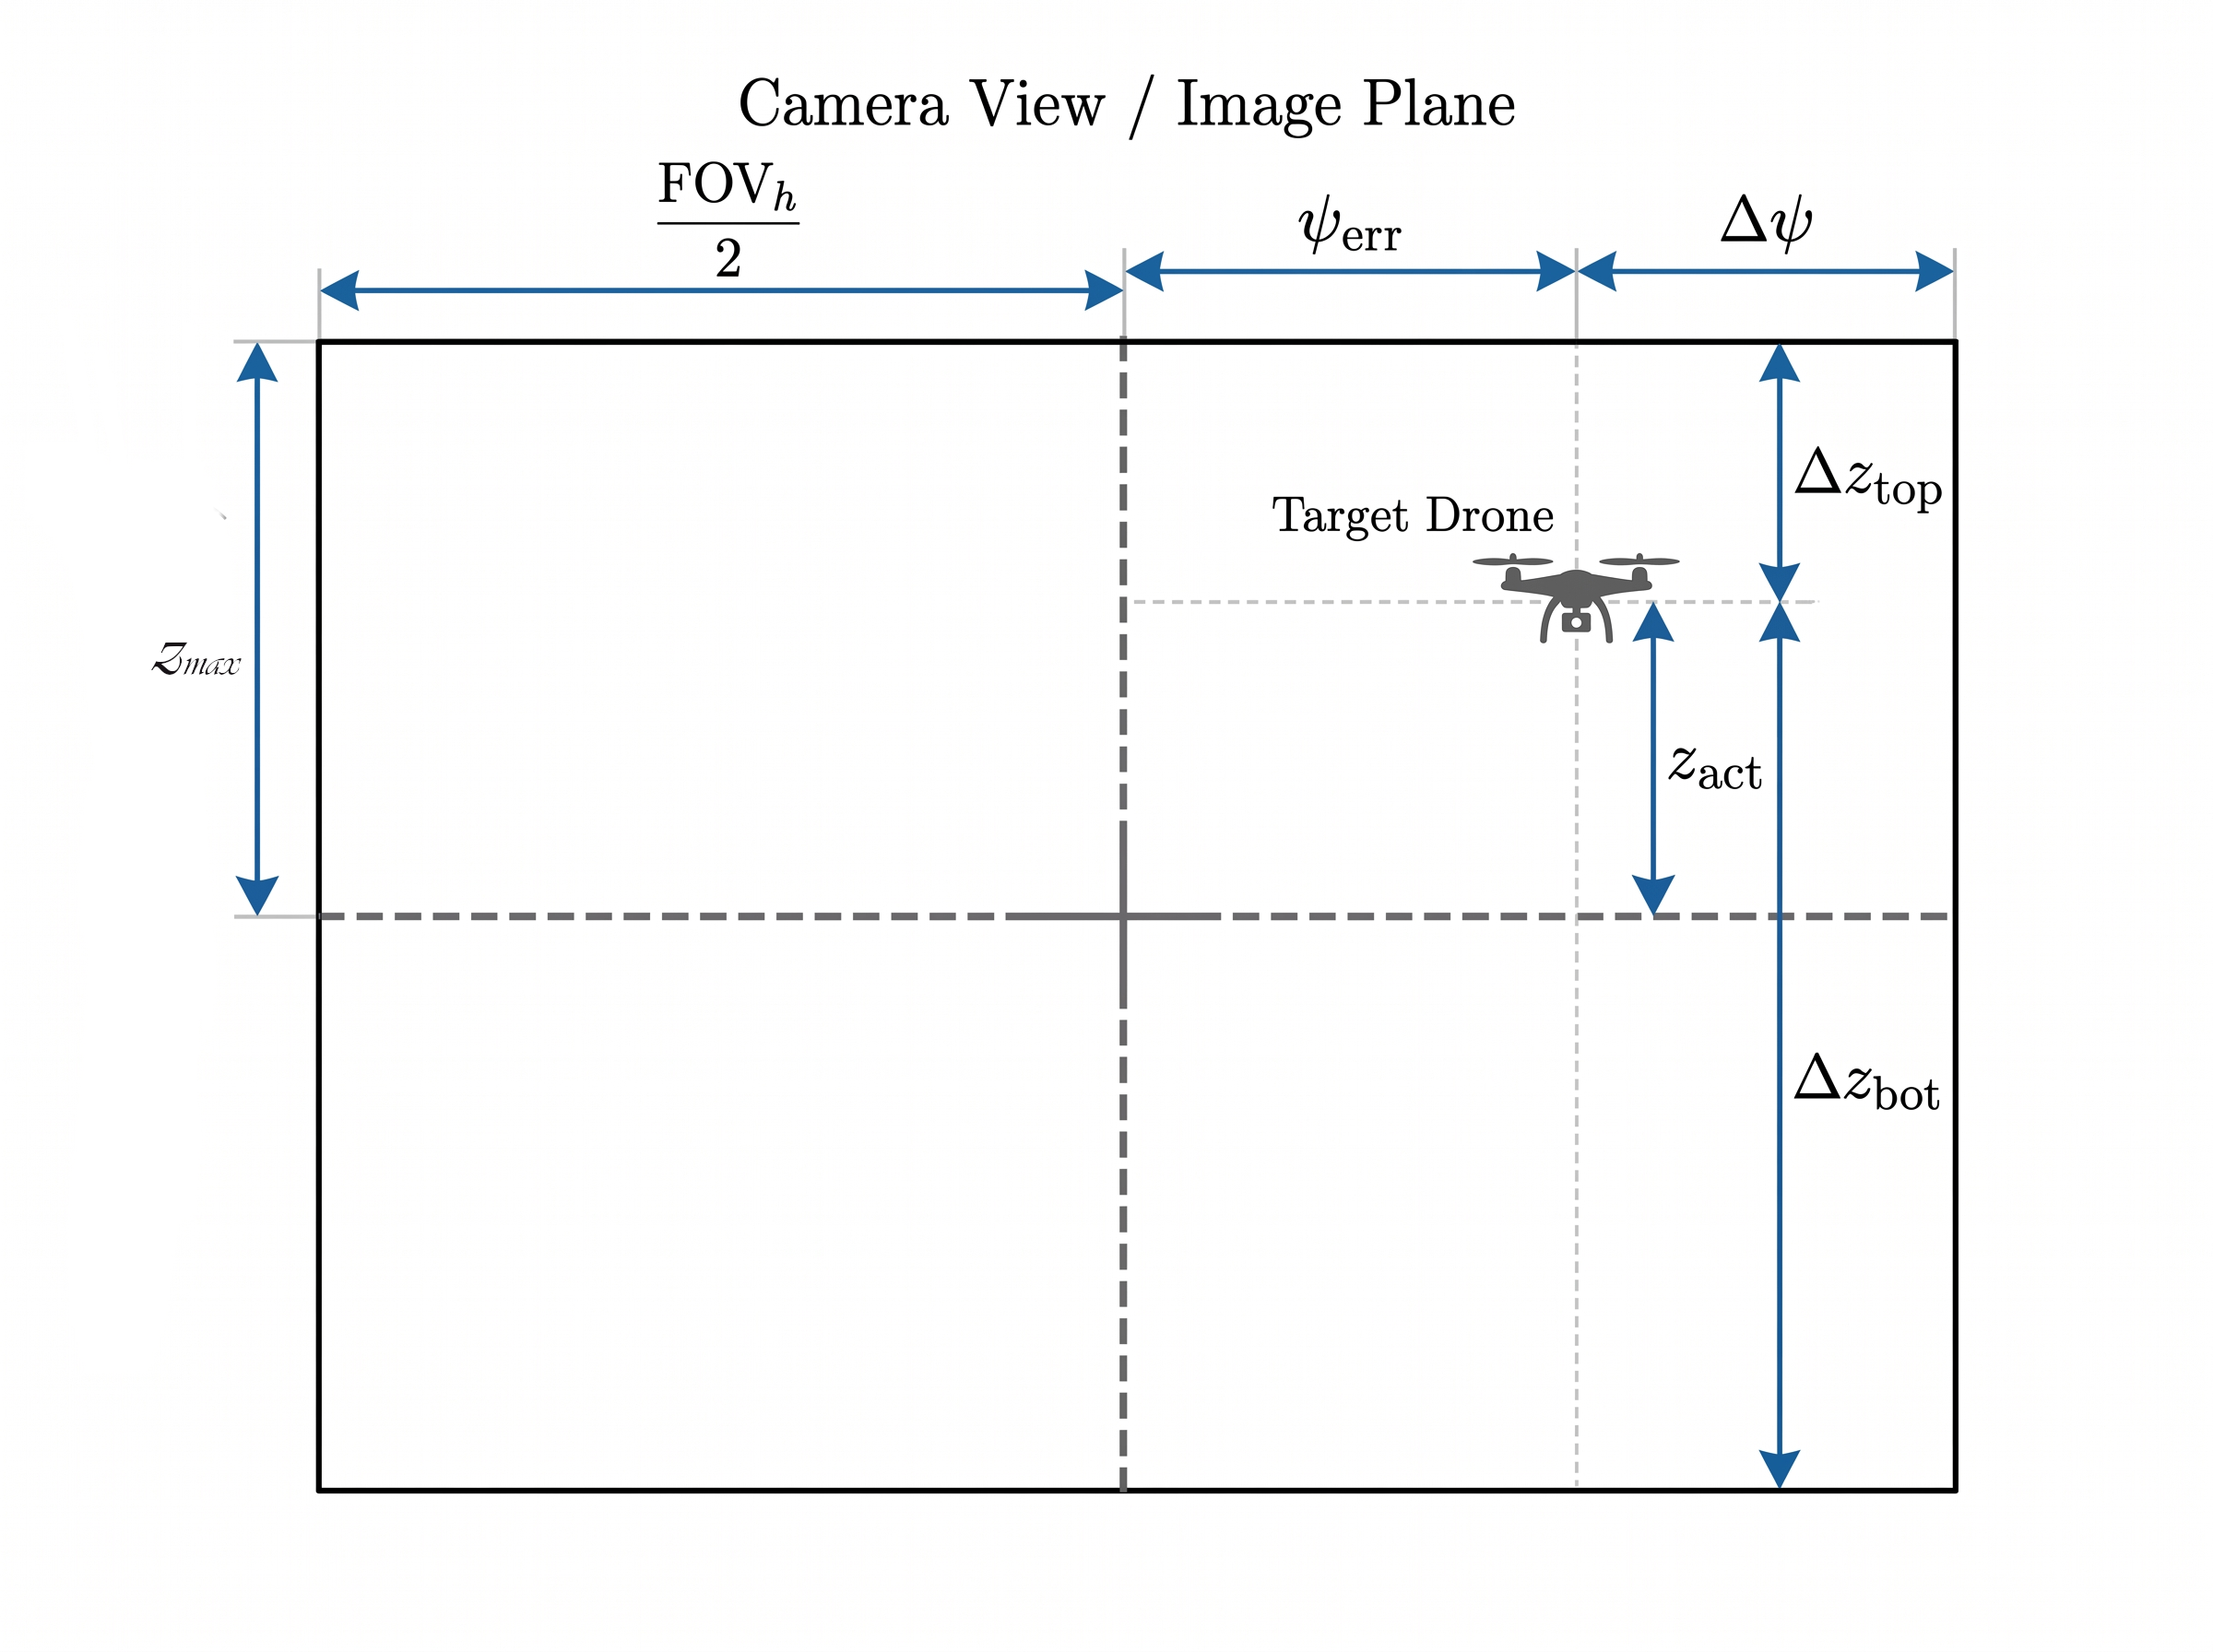
\includegraphics[width=0.8\linewidth]{Image_plane_boundaries.png}
    \caption{FOV boundaries in camera image plane}
    \label{fig:placeholder}
\end{figure}
where $r_{\min}$ ensures collision avoidance, the $z$ distances represent the remaining margins from the vertical limits of the Field of View ($\text{FOV}_v$), and $\Delta \psi$ represents the distance from the horizontal limits ($\text{FOV}_h$).
\\When any of these distances falls below a predefined activation threshold $d_{\text{act}}$, an exponential repulsive force is triggered. For a generic distance $d$, the intensity of the force is formulated as:
\begin{equation}
    \label{eq:repulsive_force}
    F_{\text{rep}}(d) = 
    \begin{cases} 
      0 & \text{if } d \geq d_{\text{act}} \\
      k_{\text{rep}} \left( e^{\left( \alpha \frac{d_{\text{act}} - d}{d_{\text{act}}} \right)} - 1 \right) & \text{if } 0 < d < d_{\text{act}} \\
      F_{\max}^{\text{rep}} & \text{if } d \leq 0
   \end{cases}
\end{equation}
where $\alpha$ is a tunable shaping factor that determines the exponential steepness of the virtual boundary, and $k_{\text{rep}}$ is the scaling gain. To satisfy the boundary condition, $k_{\text{rep}}$ is analytically derived from the maximum allowable torque $F_{\max}^{\text{rep}}$ as:
\begin{equation}
    k_{\text{rep}} = \frac{F_{\max}^{\text{rep}}}{e^\alpha - 1}
\end{equation}
In this way, the workspace is partitioned into three distinct operational regions:
\begin{itemize}
    \item \textbf{Free Region ($d \geq d_{\text{act}}$):} The vehicle is well within safe operational limits. The repulsive force is identically zero ($F_{\text{rep}} = 0$), and the operator feels only the standard centering spring-damper impedance.
    \item \textbf{Anticipatory Repulsive Buffer ($0 < d < d_{\text{act}}$):} The state enters the safety buffer. The repulsive force ramps up exponentially according to~\eqref{eq:repulsive_force}, acting as a virtual tactile barrier that warns the human pilot of the approaching boundary before any constraint violation occurs.
    \item \textbf{Violation Region ($d \leq 0$):} The boundary has been breached. The repulsive force saturates at its maximum value $F_{\max}^{\text{rep}}$ to vigorously push the operator away from danger.
\end{itemize}
The specific activation thresholds $d_{\text{act}}$ adopted in this work are configured as follows:
\begin{itemize}
    \item For the \textbf{radial distance}, $d_{\text{act}} = r_{\min} = 1.5\text{ m}$. Thus, the repulsive force activates as soon as the standoff distance drops below $r < r_{\min} + d_{\text{act}} = 3.0\text{ m}$, providing a $1.5\text{ m}$ wide progressive warning zone before reaching the minimum collision distance $r_{\min}$.
    \item For the \textbf{camera vertical FoV}, $d_{\text{act}} = 0.3 \cdot z_{\max}$. Consequently, the central $70\%$ of the image height represents a free visual zone ($F_z^{\text{rep}} = 0$), while tactile resistance activates only when the target enters the outer $30\%$ approaching the top or bottom image borders.
    \item For the \textbf{camera horizontal FoV}, $d_{\text{act}} = 0.3 \cdot (\text{FOV}_h / 2)$, applying lateral correction forces only when the yaw misalignment exceeds $70\%$ of the semi-aperture.
\end{itemize}
\begin{figure}[h!]
    \centering
    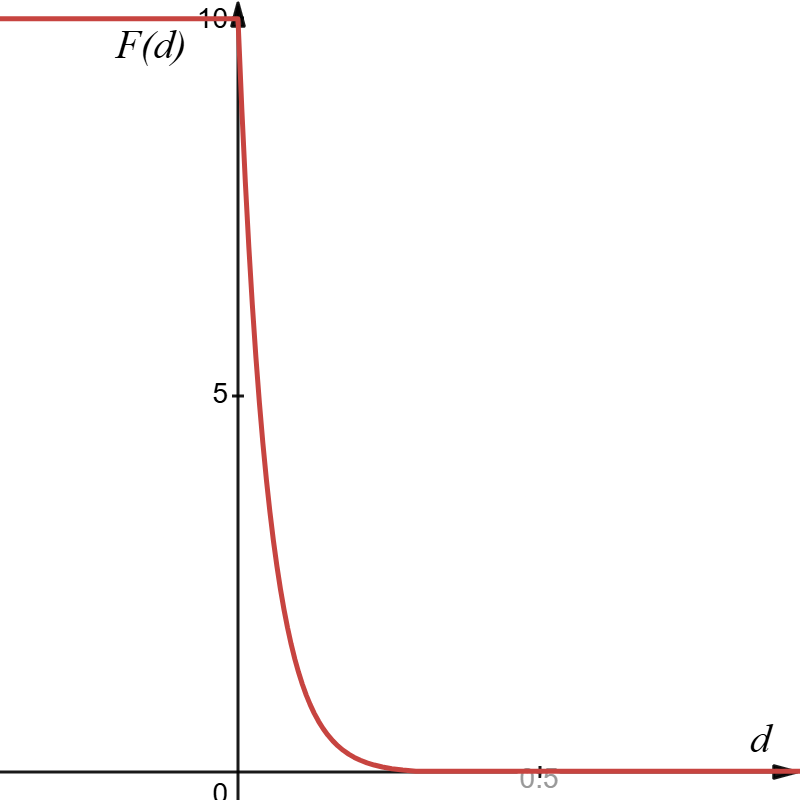
\includegraphics[width=0.6\linewidth]{Immagini/Capitolo4/F_rep.png}
    \caption{Repulsive force function $F_{rep}(d)$ - Repulsive force is maximum when $d=0$, decreases exponentially until becoming $F_{rep}=0$ N when $d\ge d_{act}$. Parameters: $\alpha=6$, $d_{act}=0.3$, $F_{max}=10$ N}
    \label{fig:placeholder}
\end{figure}
\\The   haptic interface axes $x, y$, and $z$ (defined in a standard Forward-Left-Up reference frame) directly govern the radial, azimuthal, and vertical velocity commands, respectively. Therefore, the computed scalar repulsive forces are mapped onto these corresponding operational axes to intuitively counteract unsafe human inputs:
\begin{equation}
\begin{aligned}
    F_{x}^{\text{rep}} &= F_{\text{rep}}(\Delta r) \\
    F_{y}^{\text{rep}} &= - \operatorname{sgn}(\psi_{\text{dev}}) \cdot F_{\text{rep}}(\Delta \psi) \\
    F_{z}^{\text{rep}} &= - F_{\text{rep}}(\Delta z_{\text{top}}) + F_{\text{rep}}(\Delta z_{\text{bot}})
\end{aligned}
\end{equation}
The horizontal feedback $F_{y}^{\text{rep}}$ acts directly on the yaw alignment error, pushing the operator's hand to correct tracking misalignment, while the radial and vertical forces prevent physical collisions and boundary violations.
The total force commanded to the motors of the haptic device is the superimposition of the base mechanical impedance and the visual repulsive fields, eventually saturated by the hardware limits ($F_{\max}$) to prevent mechanical damage:
\begin{equation}
    \mathbf{F}_{\text{tot}} = \operatorname{sat}\left( \mathbf{F}_{\text{imp}} + \mathbf{F}^{\text{rep}}, \pm F_{\max} \right)
\end{equation}
By combining these components, the operator naturally perceives the center of the workspace as a stable equilibrium, while the camera FOV limits and safety distances feel like elastic, repulsive walls that actively guide the teleoperation.
    \chapter{Software and Hardware Implementation}
    %\section{Hardware Architecture}
%Piattaforme aeree dei 2 droni, schede che usano, sensori usati
%\section{Software Framework}
%ROS2, integrazione con PX4,NODI PRINCIPALI COSA FANNO E CHE MESSAGGI SI SCAMBIANO, uso del bridge Micro-XRCE-DDS e modlaità offboard PX4

%\section{Optimization solver}
%DESCRIZIONE DI ACADOS E DELLE IMPOSTAZIONI DEL SOLVER USATE

This chapter details the practical implementation of the proposed cooperative aerial inspection framework. Translating the mathematical control formulation and shared control strategy into a functioning system requires a robust and real-time capable software architecture. The chapter discusses the middleware integration, the mission supervision layer, the real-time implementation of the observer drone's Non-linear Model Predictive Control (NMPC), the contact admittance filter for the inspection drone, and the haptic interface pipeline.
\section{Simulation and Hardware Setup}
The proposed framework is evaluated in both simulated and real-world environments. To ensure consistency between testing phases, the hardware and software architectures are designed to minimize the transition gap.
\\In the simulation environment, the robotic team is composed of two identical x500 quadrotor frames. The first vehicle, functioning as the Observer Drone, is equipped with a rigidly mounted virtual camera to stream the exocentric view. The second vehicle, the Inspection Drone, has a rigid link acting as an end-effector, featuring a 1D force sensor at its tip to measure environmental interaction forces during the contact task.
\begin{figure}[htbp]
    \centering
    \begin{subfigure}{0.49\textwidth}
        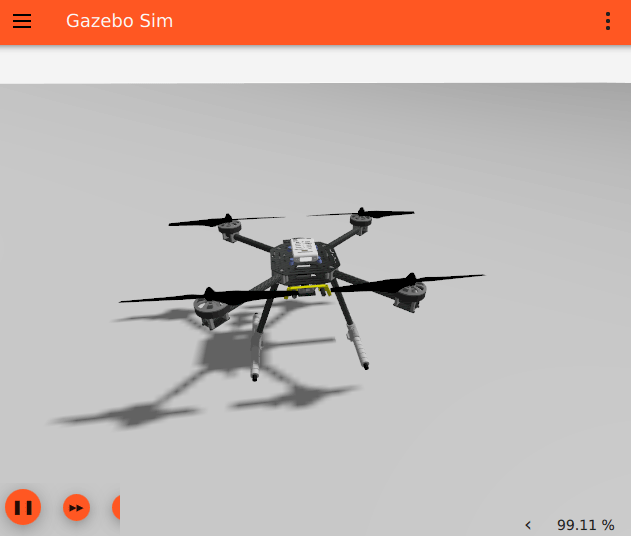
\includegraphics[width=\linewidth]{Immagini/Capitolo5/x500.DphTqKxq.png}    
    \end{subfigure}
    \begin{subfigure}{0.49\textwidth}
        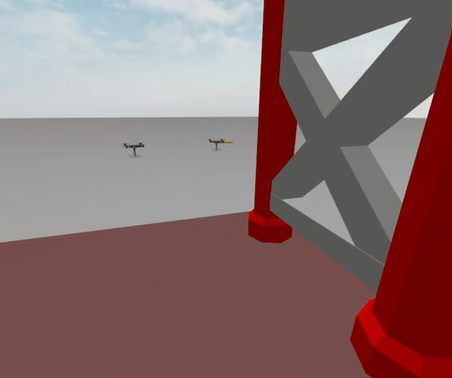
\includegraphics[width=\linewidth]{Immagini/Capitolo5/two_drones_one_bridge_2.png}    
    \end{subfigure}    
    \caption{Drones used in \texttt{SITL} simulation: x500 quadrotors - GazeboSim}
    \label{fig:placeholder}
\end{figure}
For the real-world experiments, the hardware implementation focuses entirely on validating the Observer Drone's optimal visual tracking and the associated haptic shared control. The physical Observer Drone is a custom-built octopter platform in flat configuration (whose model is mathematically equivalent to the quadrotor's one). Low-level attitude stabilization, motor mixing, and state estimation are handled by a Pixhawk flight controller. All high-level computations, including the ROS 2 middleware network, the NMPC solver, and the finite state machine, are executed onboard by a LattePanda companion computer connected to the flight controller via a serial interface.
\begin{figure}[htbp]
    \centering
    \begin{subfigure}{0.49\textwidth}
        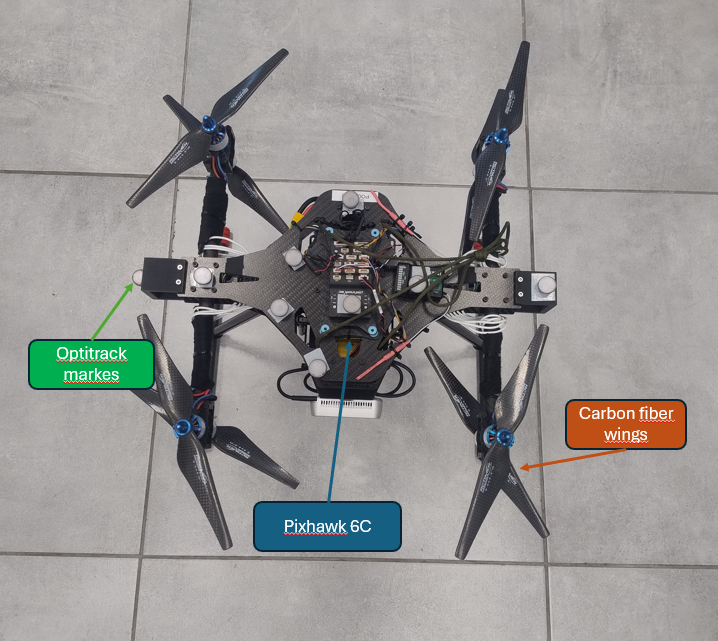
\includegraphics[width=\linewidth]{Immagini/Capitolo5/guardrone_up_labels.png}
    \label{fig:placeholder}
    \end{subfigure}
    \centering
    \begin{subfigure}{0.49\textwidth}
        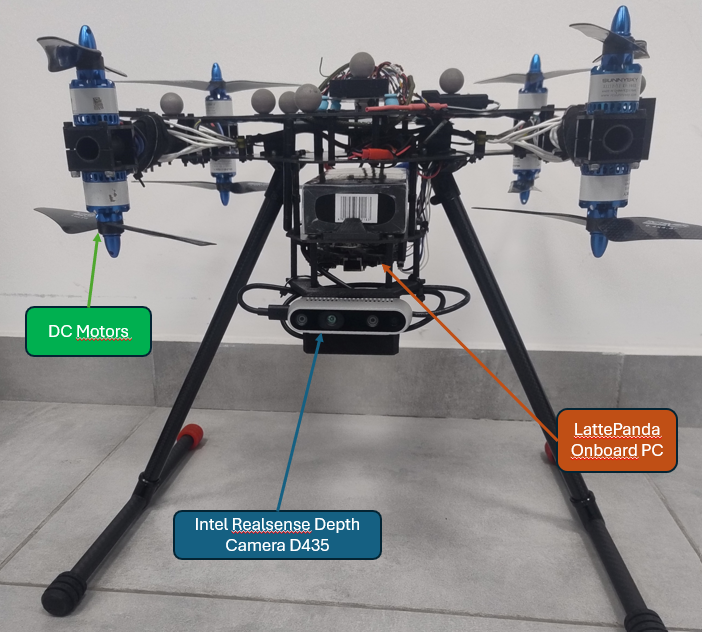
\includegraphics[width=\linewidth]{Immagini/Capitolo5/guardrone_front_labels.png}
    \label{fig:placeholder}
    \end{subfigure}
    \caption{Top and front views of real custom octocopter named \texttt{Pocho}, used for Observer UAV}
\end{figure}
Due to technical hardware constraints, the physical Inspection Drone is substituted by a manually piloted DJI quadrotor. This manually driven vehicle acts strictly as a dynamic physical target. This setup effectively tests the robustness of the observer's NMPC tracking capabilities and the human operator's haptic override in a dynamic scenario.
\section{Middleware and Simulation Architecture}
The high-level control network is developed within the Robot Operating System 2 (ROS 2) environment. ROS 2 provides a modular and distributed node architecture and relies on the Data Distribution Service (DDS) standard, ensuring the low-latency inter-process communication required for real-time control loops.
\\To interface the high-level ROS 2 network with the low-level hardware, the standard \texttt{PX4} open-source flight stack is utilized. Communication between the onboard LattePanda PC and the \texttt{Pixhawk} flight controller is handled by the \textit{Micro-XRCE-DDS} agent. This bridge directly maps the internal PX4 uORB messaging topics to ROS 2 DDS topics, allowing the control nodes to publish setpoints and read telemetry at high frequencies without custom serial protocols.
\begin{figure}[htpb]
    \centering
    \resizebox{\textwidth}{!}{% Ridimensiona in automatico ai margini della pagina
    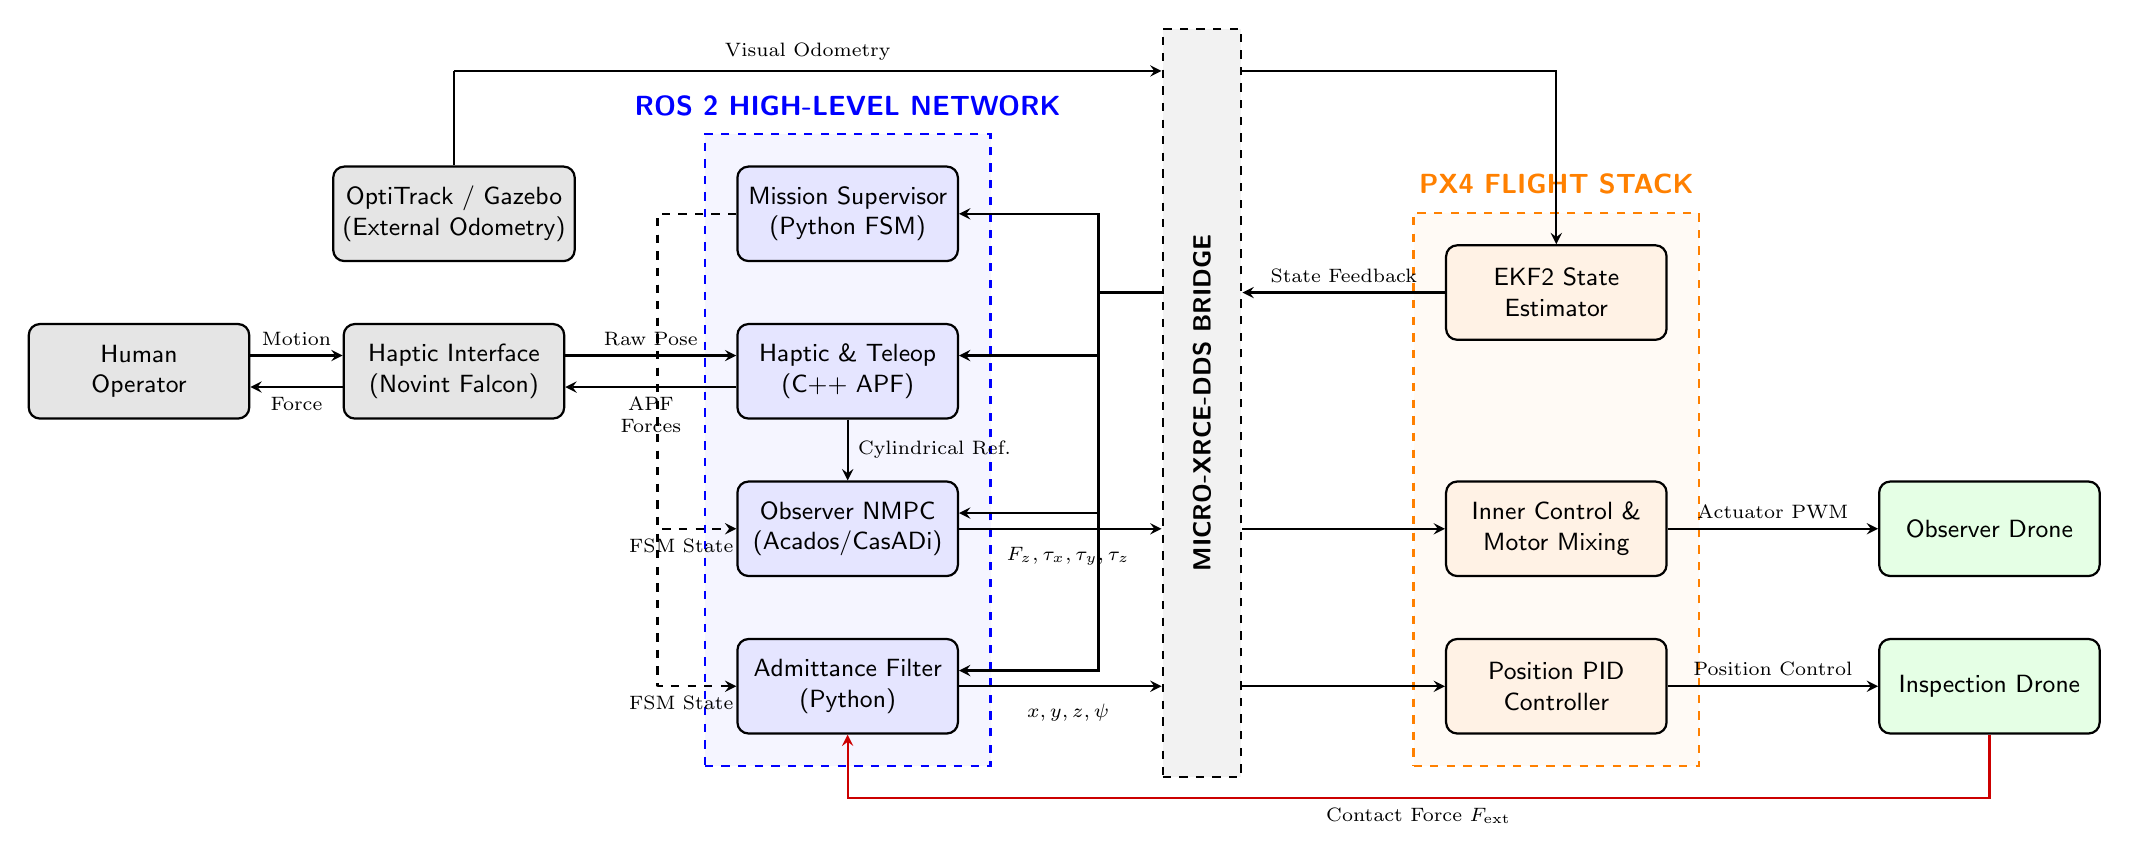
\begin{tikzpicture}[
        >=stealth,
        node distance=1.5cm and 2cm,
        box/.style={rectangle, draw=black, thick, rounded corners, align=center, minimum height=1.2cm, minimum width=2.8cm, font=\small\sffamily},
        rosbox/.style={box, fill=blue!10},
        px4box/.style={box, fill=orange!10},
        envbox/.style={box, fill=green!10},
        devbox/.style={box, fill=gray!20},
        bridge/.style={rectangle, draw=black, thick, dashed, fill=gray!10, minimum height=9.5cm, minimum width=1cm, align=center,yshift=0.6cm, font=\small\sffamily\bfseries},
        groupbox/.style={rectangle, draw=black, thick, dashed, inner sep=0.4cm, fill=black!5, fill opacity=0.2}
    ]

    % ================= NODES =================

    % Bridge
    \node[bridge] (dds) at (0, 1.5) {\rotatebox{90}{MICRO-XRCE-DDS BRIDGE}};

    % ROS 2 Nodes (Left)
    \node[rosbox] (supervisor) at (-4.5, 4.5) {Mission Supervisor \\ (Python FSM)};
    \node[rosbox] (hapticnode) at (-4.5, 2.5) {Haptic \& Teleop \\ (C++ APF)};
    \node[rosbox] (nmpc) at (-4.5, 0.5) {Observer NMPC \\ (Acados/CasADi)};
    \node[rosbox] (admittance) at (-4.5, -1.5) {Admittance Filter \\ (Python)};

    % PX4 Nodes (Right)
    \node[px4box] (ekf2) at (4.5, 3.5) {EKF2 State \\ Estimator};
    \node[px4box] (mixing) at (4.5, 0.5) {Inner Control \& \\ Motor Mixing};
    \node[px4box] (pid) at (4.5, -1.5) {Position PID \\ Controller};

    % Environment (Far Right)
    \node[envbox] (observer) at (10, 0.5) {Observer Drone};
    \node[envbox] (inspection) at (10, -1.5) {Inspection Drone};

    % Devices / Input (Far Left)
    \node[devbox] (optitrack) at (-9.5, 4.5) {OptiTrack / Gazebo \\ (External Odometry)};
    \node[devbox] (hapticdev) at (-9.5, 2.5) {Haptic Interface \\ (Novint Falcon)};
    \node[devbox] (human) at (-13.5, 2.5) {Human \\ Operator};

    % Grouping boxes (Sfondo)
% Grouping boxes (Sfondo colorato)
    \begin{scope}[on background layer]
        \node[groupbox, fit=(supervisor)(hapticnode)(nmpc)(admittance), draw=blue, fill=blue!20, label={[font=\sffamily\bfseries, text=blue, yshift=0.1cm]90:ROS 2 HIGH-LEVEL NETWORK}] (rosgroup) {}; %90 posiziona l'etichetta in alto (90 gradi)
        \node[groupbox, fit=(ekf2)(mixing)(pid), draw=orange, fill=orange!20, label={[font=\sffamily\bfseries, text=orange, yshift=0.1cm]90:PX4 FLIGHT STACK}] (px4group) {};
    \end{scope}

    % ================= ARROWS =================

    % Human <-> Haptic
    \draw[->, thick] ([yshift=0.2cm]human.east) -- node[above, font=\scriptsize] {Motion} ([yshift=0.2cm]hapticdev.west);
    \draw[<-, thick] ([yshift=-0.2cm]human.east) -- node[below, font=\scriptsize] {Force} ([yshift=-0.2cm]hapticdev.west);

    % Haptic <-> Haptic Node
    \draw[->, thick] ([yshift=0.2cm]hapticdev.east) -- node[above, font=\scriptsize] {Raw Pose} ([yshift=0.2cm]hapticnode.west);
    \draw[<-, thick] ([yshift=-0.2cm]hapticdev.east) -- node[below, font=\scriptsize, align=center] {APF\\Forces} ([yshift=-0.2cm]hapticnode.west);

    % Haptic Node -> NMPC
    \draw[->, thick] (hapticnode.south) -- node[right, font=\scriptsize] {Cylindrical Ref.} (nmpc.north);

    % OptiTrack -> Bridge -> EKF2 (CORRETTO: Passa in alto scavalcando il Supervisor)
    \draw[thick] (optitrack.north) -- ++(0, 1.2) coordinate (opti_up);
    \draw[->, thick] (opti_up) -- node[above, font=\scriptsize] {Visual Odometry} (dds.west |- opti_up);
    \draw[->, thick] (dds.east |- opti_up) -| (ekf2.north);

    % Supervisor -> NMPC & Admittance (FSM State)
    \draw[->, thick, dashed] (supervisor.west) -| ++(-1, -4.0) |- node[near end, below, font=\scriptsize,xshift=-0.2cm] {FSM State} (nmpc.west);
    \draw[->, thick, dashed] (supervisor.west) -| ++(-1, -6.0) |- node[near end, below, font=\scriptsize,xshift=-0.2cm] {FSM State} (admittance.west);

    % NMPC -> Bridge -> Mixing
    \draw[->, thick] (nmpc.east) -- node[below, font=\scriptsize,xshift=0.1cm,yshift=-0.1cm] {$F_z, \tau_x,\tau_y,\tau_z$} (dds.west |- nmpc);
    \draw[->, thick] (dds.east |- mixing) -- (mixing.west);

    % Admittance -> Bridge -> PID
    \draw[->, thick] (admittance.east) -- node[below, font=\scriptsize,xshift=0.1cm,yshift=-0.1cm] {$x,y,z,\psi$} (dds.west |- admittance);
    \draw[->, thick] (dds.east |- pid) -- (pid.west);

    % State Feedback EKF2 -> ROS Nodes
    \draw[->, thick] (ekf2.west) -- node[above, font=\scriptsize] {State Feedback} (dds.east |- ekf2);
    \draw[thick] (dds.west |- ekf2) -- ++(-0.8, 0) coordinate (state_drop);
    \draw[->, thick] (state_drop) |- (supervisor.east);
    \draw[->, thick] (state_drop) |- ([yshift=0.2cm]hapticnode.east);
    \draw[->, thick] (state_drop) |- ([yshift=0.2cm]nmpc.east);
    \draw[->, thick] (state_drop) |- ([yshift=0.2cm]admittance.east);

    % PX4 -> Environment
    \draw[->, thick] (mixing.east) -- node[above, font=\scriptsize] {Actuator PWM} (observer.west);
    \draw[->, thick] (pid.east) -- node[above, font=\scriptsize] {Position Control} (inspection.west);

    % Contact Force Loop (Inspection -> Admittance)
    \draw[->, thick, red!80!black] (inspection.south) -- ++(0, -0.8) -| node[near start, below, font=\scriptsize, text=black] {Contact Force $F_{\text{ext}}$} (admittance.south);

    \end{tikzpicture}
    }
    \caption{Block diagram of the overall hardware and software architecture, illustrating the integration between the ROS 2 high-level network and the PX4 low-level flight stack via the Micro-XRCE-DDS bridge.}
    \label{fig:architecture_diagram}
\end{figure}
\subsubsection{Software-In-The-Loop (SITL) and Gazebo}
A major advantage of this middleware integration is the ability to exploit the Software-In-The-Loop (SITL) paradigm (figure \ref{fig:architecture_diagram}). Before deployment on the physical hardware, the entire C++ control architecture was extensively validated using the PX4 SITL framework coupled with the Gazebo simulator. Gazebo simulates the rigid body dynamics, sensor noise, and environmental physics.
\\Because the Micro-XRCE-DDS bridge acts transparently, the exact same ROS 2 control nodes deployed on the LattePanda were first executed in simulation. This modularity ensures a minimal sim-to-real gap, isolating hardware-specific issues from high-level algorithmic bugs.
\\During the SITL validation, all software components- including the Gazebo simulator, the two PX4 SITL instances, and the entire ROS 2 high-level network- are executed on a single host machine. Consequently, node time synchronization and real-time message passing rely entirely on the local system clock, avoiding network-induced clock drift. The host machine utilized for these simulations is equipped with an Intel Core i9-14900HX, 32 GB of RAM, running Ubuntu 24.04 LTS.
\subsection{State Estimation}
For the MPC and haptic control loops to function effectively, an accurate 6-DoF state estimation is required. In the Gazebo SITL environment, the state is not extracted as a perfect ground truth. Instead, Gazebo simulates noisy sensor readings, which are then processed by the PX4 Extended Kalman Filter (EKF2) to generate the state estimate published on the \texttt{vehicle\_odometry} topic.
\\For the real-world setup, state estimation relies on an OptiTrack motion capture system. Rather than feeding raw OptiTrack data directly to the ROS 2 control nodes, the external tracking data is fed to the PX4 EKF2 via the \texttt{vehicle\_visual\_odometry} topic. The EKF2 fuses the external pose with high-frequency onboard IMU data. This strategy provides robust, high-frequency state feedback to the control architecture, minimizing delays and preventing solver instabilities caused by network jitter.
\section{Offboard Control Modalities}

To execute autonomous missions and override the flight controller's internal navigation logic, the system adopts the PX4 \textit{Offboard} mode. This operation mode allows a companion computer to take full authority over the vehicle by continuously streaming external setpoints via the Micro-XRCE-DDS bridge. 
\\A strict requirement of the PX4 architecture is that an \texttt{OffboardControlMode} heartbeat message must be continuously published at a minimum frequency of 2 Hz (implemented at 100 Hz in this framework). If this signal is interrupted or delayed beyond the internal timeout, the autopilot immediately drops out of offboard mode and triggers a safety failsafe, such as initiating an automatic landing. Beyond acting as a safety heartbeat, the \texttt{OffboardControlMode} message functions as a signal multiplexer: it contains boolean flags that state exactly which level of the PX4 cascaded PID hierarchy the external ROS 2 nodes intend to bypass.

\subsection{Inspection Drone: Top-Level Trajectory Planning}
For the simulated inspection drone, the physical interaction task requires tracking compliant spatial coordinates while relying on a stable baseline flight dynamics. For maximizing smoothness, point-to-point trajectories are generated by a custom trajectory generator. This module computes trapezoidal velocity profiles for both the 3D spatial position and the yaw angle, ensuring bounded accelerations.
\\The resulting smooth kinematic references, which are continuously modified by the admittance filter upon environmental contact, are inserted at the very top of the PX4 control cascade. To enable this, the \texttt{OffboardControlMode} message is configured with the \texttt{position} flag set to true, and the targets are published via the \texttt{TrajectorySetpoint} message.

\subsection{Observer Drone: NMPC and Low-Level Actuation}
The observer drone utilizes a hybrid approach. The NMPC is formulated to act simultaneously as an optimal trajectory planner and a dynamic controller. However, nonlinear optimal controllers depend, of course, on actual optimization cost variables, e.g. where the other drone is located, its position in the camera frame, and so on. 
\\Therefore, the observer drone executes its initial vertical takeoff relying on the standard PX4 position controller, utilizing the exact same \texttt{TrajectorySetpoint} modality described for the inspection drone. Once the vehicle reaches the predefined hovering altitude and stabilizes, a safe-switch routine is triggered. The control node dynamically flips the \texttt{OffboardControlMode} flags, disabling the position cascaded loops and enabling direct motor actuation.
\\During this NMPC active phase, the architecture completely bypasses the autopilot's position, velocity, and attitude controllers. The node computes the optimal normalized body thrust and body torques, injecting them directly at the lowest level via the \texttt{VehicleThrustSetpoint} and \texttt{VehicleTorqueSetpoint} messages. Special care is taken to map the optimal control variables into the autopilot's native internal frame (Front-Right-Down, FRD).

\section{Haptic interface}
To bridge the human operator with the multi-agent system (figure \ref{fig:haptic_mapping_logic}), the haptic teleoperation logic is implemented as a dedicated ROS 2 C++ node (\texttt{fd\_haptic\_joy\_node}). The use of C++ is preferred to process hardware callbacks and compute the Artificial Potential Field (APF) forces without introducing delays typical of interpreted languages.
\\The node interacts with the physical Novint Falcon through the Force Dimension SDK, wrapped within a \texttt{ros2\_control} hardware interface. To enable the dual-drone shared control paradigm, the native device driver and the state broadcasters were modified. Instead of exposing a single generic clutch button, the hardware interface reads and broadcasts the binary state of all four physical buttons of the Falcon via the \texttt{/fd/button\_states} topic. This allows the control node to act as a signal multiplexer: pressing the center button routes the joystick commands to dynamically alter the Observer Drone's cylindrical Point of View, while pressing the upper button activates the Cartesian teleoperation of the Inspection Drone.
\\The node executes its logic through a strict 100 Hz \texttt{wall\_timer}. At each control cycle ($dt = 10\text{ ms}$), the node performs the following pipeline:
\begin{enumerate}
    \item \textbf{Kinematic Mapping:} The raw end-effector position of the haptic device is mapped from its native hardware frame to the standard ROS 2 FLU (Forward-Left-Up) coordinate system (for more details see \ref{app:implementation_details}). A non-linear deadband ($0.008\text{ m}$) filters out sensor noise and unintentional hand tremors.
    \item \textbf{Reference Integration:} Based on the active button state, the filtered displacements are scaled by a kinematic gain and integrated into velocity commands. The node then publishes the updated setpoints to either the \texttt{/NMPC\_haptic\_ref} topic (for the NMPC) or the \texttt{/interaction\_live\_pose} topic (for the admittance planner).
    \item \textbf{Force Feedback Rendering:} Concurrently, the node calculates the base mechanical impedance (virtual spring-damper) and the APF repulsive forces based on the actual telemetry of the active drone. The total computed wrench is saturated to a hardware limit of $\pm 10\text{ N}$ to protect the mechanical actuators and published directly to the \texttt{ros2\_control} command topic (\texttt{/fd/fd\_controller/commands}).

\begin{figure}[h!]
    \centering
    \resizebox{0.95\textwidth}{!}{
    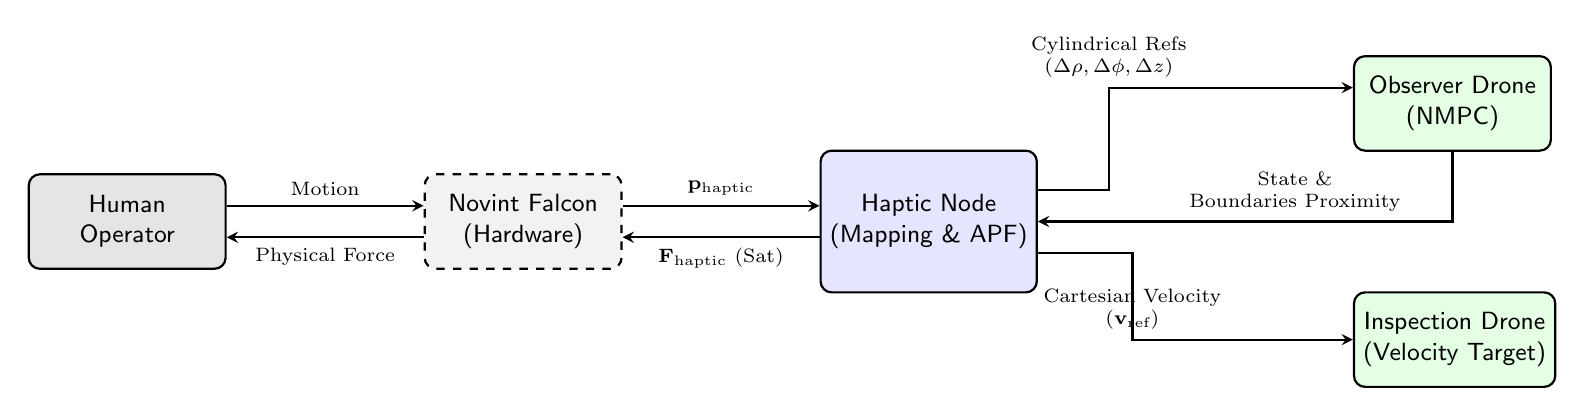
\begin{tikzpicture}[
        >=stealth,
        node distance=2cm and 2.5cm,
        box/.style={rectangle, draw=black, thick, rounded corners, align=center, minimum height=1.2cm, minimum width=2.5cm, font=\small\sffamily},
        humanbox/.style={box, fill=gray!20},
        devicebox/.style={box, fill=gray!10, dashed},
        rosbox/.style={box, fill=blue!10},
        dronebox/.style={box, fill=green!10}
    ]

    % ================= NODES =================
    \node[humanbox] (human) {Human \\ Operator};
    
    \node[devicebox, right=of human] (falcon) {Novint Falcon \\ (Hardware)};
    
    \node[rosbox, right=of falcon, minimum height=1.8cm] (hapticnode) {Haptic Node \\ (Mapping \& APF)};

    % Drones
    \node[dronebox, right=of hapticnode, yshift=1.5cm, xshift=1.5cm] (observer) {Observer Drone \\ (NMPC)};
    \node[dronebox, right=of hapticnode, yshift=-1.5cm, xshift=1.5cm] (inspection) {Inspection Drone \\ (Velocity Target)};

    % ================= ARROWS =================

    % Human <-> Falcon
    \draw[->, thick] ([yshift=0.2cm]human.east) -- node[above, font=\scriptsize] {Motion} ([yshift=0.2cm]falcon.west);
    \draw[<-, thick] ([yshift=-0.2cm]human.east) -- node[below, font=\scriptsize] {Physical Force} ([yshift=-0.2cm]falcon.west);

    % Falcon <-> ROS Node
    \draw[->, thick] ([yshift=0.2cm]falcon.east) -- node[above, font=\scriptsize] {$\mathbf{p}_{\text{haptic}}$} ([yshift=0.2cm]hapticnode.west);
    \draw[<-, thick] ([yshift=-0.2cm]falcon.east) -- node[below, font=\scriptsize] {$\mathbf{F}_{\text{haptic}}$ (Sat)} ([yshift=-0.2cm]hapticnode.west);

    % ROS Node -> Observer (Upper branch)
    \draw[->, thick] ([yshift=0.4cm]hapticnode.east) -- ++(0.9,0) |- node[above, font=\scriptsize, align=center] {Cylindrical Refs \\ ($\Delta\rho, \Delta\phi, \Delta z$)} ([yshift=0.2cm]observer.west);
    
    % Observer -> ROS Node (Feedback)
    \draw[<-, thick] ([yshift=0cm]hapticnode.east) -- ++(3,0) -| node[above, font=\scriptsize, align=center,xshift=-2cm] {State \& \\Boundaries Proximity} ([yshift=0cm]observer.south);

    % ROS Node -> Inspection (Lower branch - open loop)
    \draw[->, thick] ([yshift=-0.4cm]hapticnode.east) -- ++(1.2,0) |- node[above, font=\scriptsize, align=center] {Cartesian Velocity \\ ($\mathbf{v}_{\text{ref}}$)} (inspection.west);

    \end{tikzpicture}
    }
    \caption{Logical block diagram of the haptic teleoperation interface, illustrating the asymmetric control mapping: bilateral feedback loop for the Observer Drone versus open-loop Cartesian velocity control for the Inspection Drone.}
    \label{fig:haptic_mapping_logic}
\end{figure}

\end{enumerate}
\section{Mission Supervisor}
To ensure a safe and predictable execution of the cooperative task, the overall mission logic is centralized in a dedicated Python node acting as a Finite State Machine (FSM). Rather than computing continuous trajectories, this node operates as a high-level discrete event controller. It manages state transitions, monitors system health, and dispatches system-level instructions to the flight controllers. Figure \ref{fig:supervisor_architecture} illustrates the software architecture and discrete-event execution flow of the supervisor node.

\begin{figure}[htbp]
    \centering
    \resizebox{\textwidth}{!}{%
    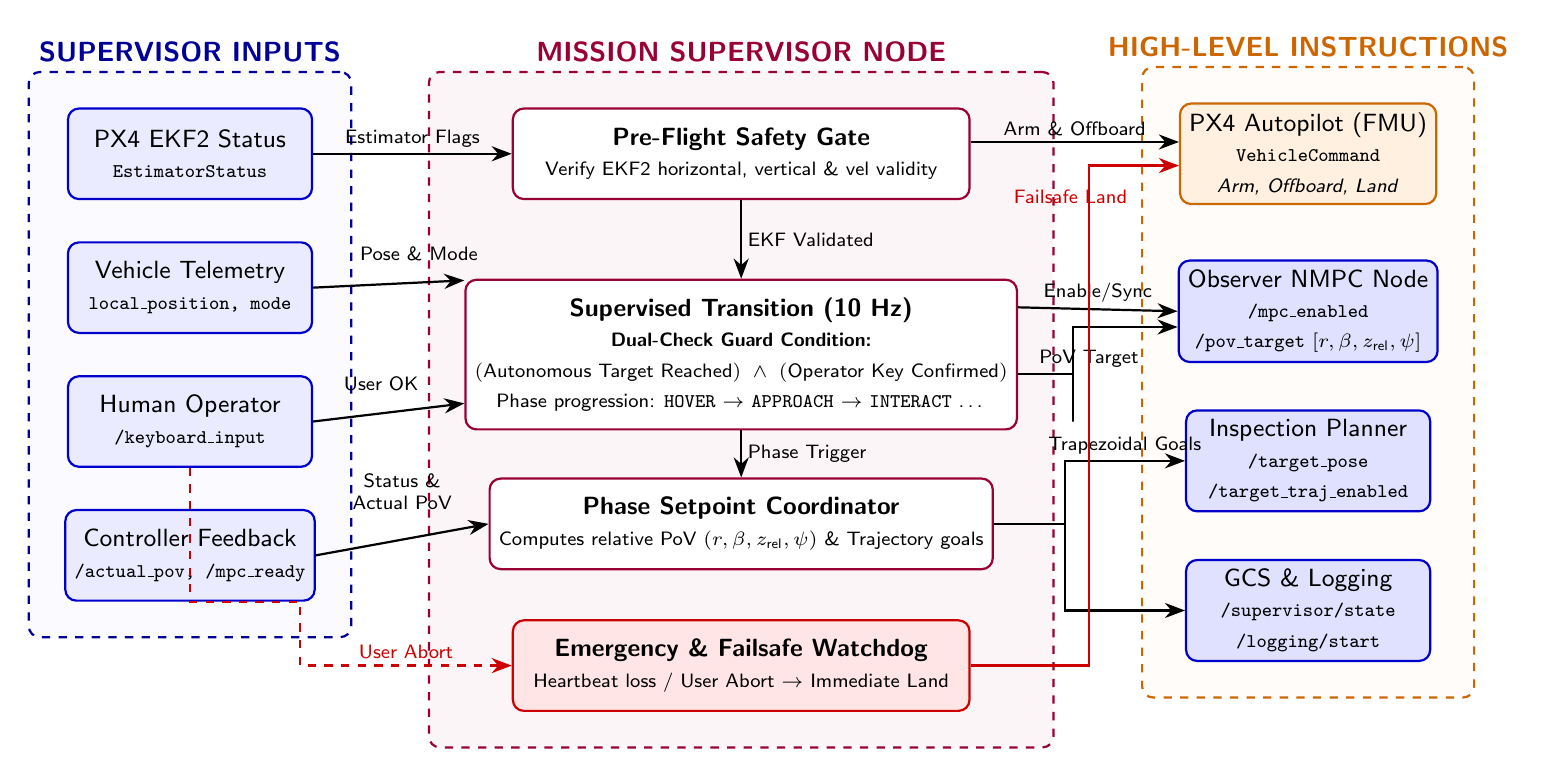
\begin{tikzpicture}[
        >=stealth,
        node distance=1.2cm and 2.0cm,
        box/.style={rectangle, draw=black, thick, rounded corners, align=center, minimum height=1.15cm, minimum width=3.1cm, font=\small\sffamily},
        inbox/.style={box, fill=blue!8, draw=blue!80!black},
        corebox/.style={box, fill=white, draw=purple!80!black, thick},
        alertbox/.style={box, fill=red!10, draw=red!80!black, thick},
        outpx4/.style={box, fill=orange!12, draw=orange!80!black},
        outros/.style={box, fill=blue!12, draw=blue!80!black},
        groupbox/.style={rectangle, draw=#1, thick, dashed, inner sep=0.45cm, rounded corners},
        labeltext/.style={font=\scriptsize\sffamily, fill opacity=1, inner sep=2pt, align=center}
    ]

    % ================= INPUTS (COLONNA SINISTRA) =================
    \node[inbox] (in_ekf) at (0, 3.2) {PX4 EKF2 Status \\ \scriptsize\texttt{EstimatorStatus}};
    \node[inbox] (in_telemetry) at (0, 1.5) {Vehicle Telemetry \\ \scriptsize\texttt{local\_position, mode}};
    \node[inbox] (in_human) at (0, -0.2) {Human Operator \\ \scriptsize\texttt{/keyboard\_input}};
    \node[inbox] (in_planner) at (0, -1.9) {Controller Feedback \\ \scriptsize\texttt{/actual\_pov, /mpc\_ready}};

    % ================= SUPERVISOR CORE (COLONNA CENTRALE) =================
    \node[corebox, minimum width=5.8cm] (gate_ekf) at (7.0, 3.2) {
        \textbf{Pre-Flight Safety Gate} \\
        \scriptsize Verify EKF2 horizontal, vertical \& vel validity
    };

    \node[corebox, minimum width=5.8cm, minimum height=1.9cm] (fsm_engine) at (7.0, 0.65) {
        \textbf{Supervised Transition (10 Hz)} \\
        \scriptsize \textbf{Dual-Check Guard Condition:} \\
        \scriptsize $(\text{Autonomous Target Reached}) \;\wedge\; (\text{Operator Key Confirmed})$ \\
        \scriptsize Phase progression: \texttt{HOVER} $\rightarrow$ \texttt{APPROACH} $\rightarrow$ \texttt{INTERACT} \dots
    };

    \node[corebox, minimum width=5.8cm] (setpoint_gen) at (7.0, -1.5) {
        \textbf{Phase Setpoint Coordinator} \\
        \scriptsize Computes relative PoV $(r, \beta, z_{\text{rel}}, \psi)$ \& Trajectory goals
    };

    \node[alertbox, minimum width=5.8cm] (watchdog) at (7.0, -3.3) {
        \textbf{Emergency \& Failsafe Watchdog} \\
        \scriptsize Heartbeat loss / User Abort $\rightarrow$ Immediate Land
    };

    % ================= OUTPUTS (COLONNA DESTRA) =================
    \node[outpx4] (out_px4) at (14.2, 3.2) {
        PX4 Autopilot (FMU) \\
        \scriptsize\texttt{VehicleCommand} \\
        \scriptsize\textit{Arm, Offboard, Land}
    };

    \node[outros] (out_nmpc) at (14.2, 1.2) {
        Observer NMPC Node \\
        \scriptsize\texttt{/mpc\_enabled} \\
        \scriptsize\texttt{/pov\_target} $[r, \beta, z_{\text{rel}}, \psi]$
    };

    \node[outros] (out_planner) at (14.2, -0.7) {
        Inspection Planner \\
        \scriptsize\texttt{/target\_pose} \\
        \scriptsize\texttt{/target\_traj\_enabled}
    };

    \node[outros] (out_gcs) at (14.2, -2.6) {
        GCS \& Logging \\
        \scriptsize\texttt{/supervisor/state} \\
        \scriptsize\texttt{/logging/start}
    };

    % ================= BACKGROUND BOXES =================
    \begin{scope}[on background layer]
        % Box Supervisore
        \node[groupbox=purple!80!black, fit=(gate_ekf) (fsm_engine) (setpoint_gen) (watchdog), fill=purple!4] (supbox) {};
        \node[above, font=\sffamily\bfseries\color{purple!80!black}] at (supbox.north) {MISSION SUPERVISOR NODE};

        % Box Inputs
        \node[groupbox=blue!60!black, fit=(in_ekf) (in_telemetry) (in_human) (in_planner), fill=blue!2] (inpbox) {};
        \node[above, font=\sffamily\bfseries\color{blue!60!black}] at (inpbox.north) {SUPERVISOR INPUTS};

        % Box Outputs
        \node[groupbox=orange!80!black, fit=(out_px4) (out_nmpc) (out_planner) (out_gcs), fill=orange!2] (outbox) {};
        \node[above, font=\sffamily\bfseries\color{orange!80!black}] at (outbox.north) {HIGH-LEVEL INSTRUCTIONS};
    \end{scope}

    % ================= FRECCE E COLLEGAMENTI =================
    % Inputs -> Supervisor
    \draw[-{Stealth[scale=1.1]}, thick] (in_ekf.east) -- node[above, labeltext] {Estimator Flags} (gate_ekf.west);
    \draw[-{Stealth[scale=1.1]}, thick] (in_telemetry.east) -- node[above, labeltext, pos=0.7,yshift=0.2cm] {Pose \& Mode} (fsm_engine.165);
    \draw[-{Stealth[scale=1.1]}, thick] (in_human.east) -- node[above, labeltext, pos=0.45,yshift=0.2cm] {User OK} (fsm_engine.190);
    \draw[-{Stealth[scale=1.1]}, thick] (in_planner.east) -- node[above, labeltext,yshift=0.3cm] {Status \& \\Actual PoV} (setpoint_gen.west);

    % Interni Supervisor
    \draw[-{Stealth[scale=1.1]}, thick] (gate_ekf.south) -- node[right, labeltext] {EKF Validated} (fsm_engine.north);
    \draw[-{Stealth[scale=1.1]}, thick] (fsm_engine.south) -- node[right, labeltext] {Phase Trigger} (setpoint_gen.north);
    \draw[-{Stealth[scale=1.1]}, thick, dashed, red!80!black] (in_human.south) |- ++(1.4, -1.7) |- node[near end, above, labeltext, text=red!80!black] {User Abort} (watchdog.west);

    % Supervisor -> Outputs
    \draw[-{Stealth[scale=1.1]}, thick] ([yshift=0.15cm]gate_ekf.east) -- node[above, labeltext] {Arm \& Offboard} ([yshift=0.15cm]out_px4.west);
    \draw[-{Stealth[scale=1.1]}, thick] ([yshift=0.6cm]fsm_engine.east) -- node[above, labeltext] {Enable/Sync} (out_nmpc.west);
    \draw[-{Stealth[scale=1.1]}, thick] ([yshift=-0.25cm]fsm_engine.east) -| ++(0.7, -0.6) |- node[near start, above, labeltext, xshift=2mm] {PoV Target} ([yshift=-0.2cm]out_nmpc.west);
    \draw[-{Stealth[scale=1.1]}, thick] (setpoint_gen.east) -| ++(0.9, 0.4) |- node[near end, above, labeltext] {Trapezoidal Goals} (out_planner.west);
    \draw[-{Stealth[scale=1.1]}, thick] (setpoint_gen.east) -| ++(0.9, -0.7) |- (out_gcs.west);
    
    % Failsafe Land arrow
    \draw[-{Stealth[scale=1.1]}, thick, red!80!black] (watchdog.east) -| ++(1.5, 0) |- node[near end, left, labeltext, text=red!80!black, yshift=-4mm] {Failsafe Land} ([yshift=-0.15cm]out_px4.west);

    \end{tikzpicture}%
    }
    \caption{Architecture and execution flow of the Mission Supervisor node. The node centralizes telemetry inputs, EKF2 safety checks, and operator confirmations to handle PX4 flight modes and give phase-dependent targets to the UAVs.}
    \label{fig:supervisor_architecture}
\end{figure}

\subsection{Initialization and Safety Checks}
Before allowing any actuation, the supervisor initializes by subscribing to the telemetry topics of the active drones. A critical safety constraint is the state estimation validity. The node actively monitors the \texttt{EstimatorStatus} uORB message generated by the PX4 Extended Kalman Filter (EKF2). The FSM remains locked in the \textit{Wait EKF} state until the specific flags indicating horizontal position, vertical position, and velocity convergence are all confirmed as valid by the autopilot. This prevents the system from attempting an autonomous takeoff with severely degraded state estimates.
\subsection{System Commands and Supervised Autonomy}
When the initialization conditions are met, the FSM progression is governed by a supervised autonomy paradigm. Transitions between major operational phases (e.g., Takeoff, Approach, Interaction, Detachment) are not triggered purely by geometric thresholds, but are guarded by human-in-the-loop confirmations acquired via keyboard callbacks.
\\Upon receiving confirmation for a phase transition, the supervisor node sends hardware-level instructions using the \texttt{VehicleCommand} message structure. For instance, to initiate the mission, the node sends a \texttt{VEHICLE\_CMD\_DO\_SET\_MODE} command to force the Offboard mode, immediately followed by a \texttt{VEHICLE\_CMD\_\\COMPONENT\_ARM\_DISARM} command to arm the motors. 
\subsection{Emergency Handling and Hardware deployment}
A background routine within the supervisor continuously monitors the offboard status and the human operator's inputs. If a manual stop is triggered, or if the system detects an unexpected drop out of the offboard mode, the FSM instantly transitions to an \textit{Emergency} state. In this state, the node overrides any active MPC or admittance reference and publishes a \texttt{VEHICLE\_CMD\_NAV\_LAND} command, forcing the UAVs to descend safely at their current planar coordinates.

    \chapter{Simulation Results}
    \label{ch:results}
To validate the proposed cooperative multi-drone architecture, a comprehensive testing campaign was conducted. The evaluation follows this approach: first planners and controllers are validated in a simulated environment, then the human-in-the-loop haptic interactions are analyzed, and finally the complete cooperative mission is shown. A preliminary assessment of the physical real-world setup concludes the chapter.

\section{Software-in-the-Loop Setup}
The simulated validation was performed using the Gazebo physics engine, fully integrated with the PX4 Autopilot Software-in-the-Loop (SITL) environment and ROS 2 Humble. The multi-vehicle setup relies on the Micro-XRCE-DDS bridge to independently handle the uORB messaging for two virtual standard \texttt{x500} quadrotor frames. 
\\To replicate the computational constraints of the real onboard companion computer, the NMPC solver was configured with a strict execution constraint of $100$ Hz (sampling time $T_s = 10$ ms) over a prediction horizon of $N=15$ steps. The state and control weighting matrices ($\mathbf{Q}$ and $\mathbf{R}$) were tuned empirically to prioritize visual constraints (e.g., locking the relative height and radial distance) while heavily penalizing aggressive torque variations, ensuring a smooth video feed. 
\begin{table}[htbp]
\centering
\caption{Parameters and weight matrices in NMPC. Notice: $\Delta_{max}$, used for weights normalization, is intended as maximum acceptable displacement with respect correspondent reference}
\label{tab:nmpc_parameters}
\small
\begin{tabular}{llcccc}
\toprule
 \textbf{Symbol} & \textbf{Range $\Delta_{\max}$} & \textbf{Priority $w$} & \textbf{Value (Scalar/Diagonal)} \\
\midrule
\multicolumn{4}{l}{} \\
$T_s$            & ---                                   & ---                   & \SI{10}{\milli\second} (\SI{100}{\hertz}) \\
$N$              & ---                                   & ---                   & $15$ \\
$T_p = N T_s$    & ---                                   & ---                   & \SI{0.5}{\second} \\
\midrule
\multicolumn{4}{l}{\textit{State cost terms ($Q$)}} \\
$p_{x}, p_{y}$   & \SI{0.20}{\meter}                     & $10.0$                & $250.0$ \\
$p_{z}$          & \SI{0.15}{\meter}                     & $10.0$                & $444.4$ \\
$\psi$           & $\pi/4\ \si{\radian}$ (\ang{45})      & $10.0$                & $16.21$ \\
$v_x, v_y, v_z$  & \SI{0.20}{\meter\per\second}          & $2.0$                 & $50.0$ \\
$\omega_x, \omega_y$ & \SI{0.15}{\radian\per\second}     & $0.20$                & $8.89$ \\
$\omega_z$       & \SI{0.40}{\radian\per\second}         & $0.20$                & $1.25$ \\
$a_x, a_y, a_z$  & \SI{0.20}{\meter\per\second\squared}  & $0.33$                & $8.33$ \\
$j_x, j_y, j_z$  & \SI{4.0}{\meter\per\second\cubed}     & $0.10$                & $6.25 \times 10^{-3}$ \\
$s_x, s_y, s_z$  & \SI{20.0}{\meter\per\second\tothe{4}} & $0.10$                & $2.50 \times 10^{-4}$ \\
\midrule
\multicolumn{4}{l}{\textit{Input cost terms ($R$)}} \\
$F_z$            & \SI{0.50}{\newton}                    & $0.10$                & $0.40$ \\
$\tau_x, \tau_y$ & \SI{0.20}{\newton\meter}              & $0.10$                & $2.50$ \\
$\tau_z$         & \SI{0.50}{\newton\meter}              & $0.10$                & $0.40$ \\
\bottomrule
\end{tabular}
\end{table}


\section{NMPC Hovering and Tracking Validation}
Before introducing the autonomous switching references or human commands, a baseline validation of the Observer Drone's NMPC was performed. The objective of this isolated test is to demonstrate the stability of the optimal solver, the safety of the PID-to-NMPC switch, and the real-time computational feasibility.
\\During this test, the drone performs an autonomous vertical takeoff using the native PX4 position controller. Upon reaching the predefined hovering altitude, the safe-switch logic brings the drone into offboard thrust and torque mode. The only conceptual difference is that after the switch the observer drone keeps the other drone centered in image plane; this is a design choice. Another one could have been ignoring the yaw, that is, compensating for it and shifting it a way not to turn.
\begin{figure}[h!]
\centering
\begin{subfigure}[b]{0.51\textwidth}
    
\includegraphics[width=\linewidth]{Immagini/Capitolo6/Simulations/Hovering/phases_legend.pdf}
\end{subfigure}
\begin{subfigure}[b]{0.49\textwidth}
    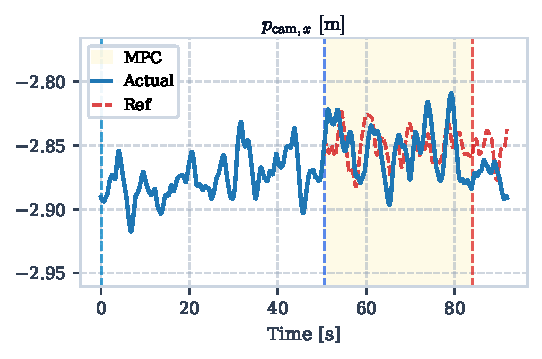
\includegraphics[width=\linewidth]{Immagini/Capitolo6/Simulations/Hovering/POS_cam_x.pdf}
    \label{fig:placeholder}
\end{subfigure}
\begin{subfigure}[b]{0.49\textwidth}
    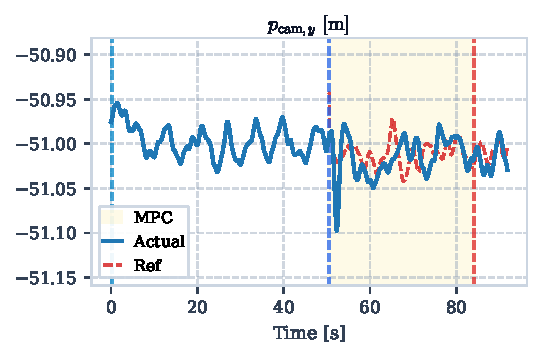
\includegraphics[width=\linewidth]{Immagini/Capitolo6/Simulations/Hovering/POS_cam_y.pdf}
    \label{fig:placeholder}
\end{subfigure}
\begin{subfigure}[b]{0.49\textwidth}
    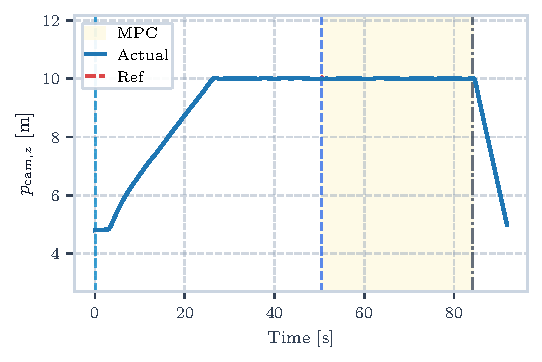
\includegraphics[width=\linewidth]{Immagini/Capitolo6/Simulations/Hovering/POS_cam_z.pdf}
    \label{fig:placeholder}
\end{subfigure}
\begin{subfigure}[b]{0.49\textwidth}
    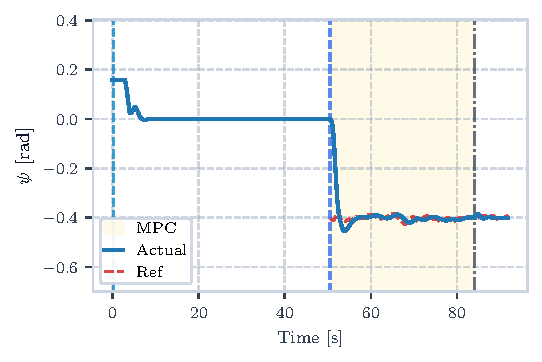
\includegraphics[width=\linewidth]{Immagini/Capitolo6/Simulations/Hovering/YAW_yaw_actual_vs_desired.pdf}
    \label{fig:placeholder}
\end{subfigure}
\caption{Cartesian coordinates of Observer Drone camera in ENU frame}
\label{fig:hovering_pos}
\end{figure}
\\As shown in Figure \ref{fig:hovering_pos}, the NMPC successfully maintains the hovering flight dynamics. Mostly important, the transition between the two controllers is without any transient instability or loss of altitude. 
The yaw smoothly reaches a zero-error steady state, while 3D position of the drone is kept around hovering position, with performances comparable to the standard PID-hovering.
\begin{figure}[h!]
\centering
\begin{subfigure}[b]{0.51\textwidth}
    
\includegraphics[width=\linewidth]{Immagini/Capitolo6/Simulations/Hovering/phases_legend.pdf}
\end{subfigure}
\begin{subfigure}[b]{0.49\textwidth}
    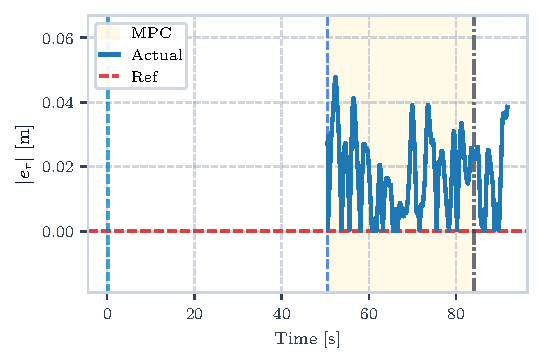
\includegraphics[width=\linewidth]{Immagini/Capitolo6/Simulations/Hovering/CYL_POV_ERR_distance_error_r_cyl_err.pdf}
    \label{fig:placeholder}
\end{subfigure}
\begin{subfigure}[b]{0.49\textwidth}
    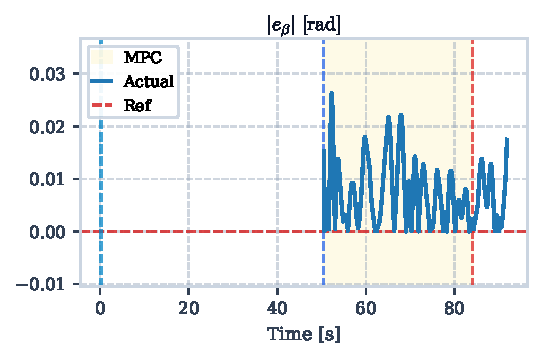
\includegraphics[width=\linewidth]{Immagini/Capitolo6/Simulations/Hovering/CYL_POV_ERR_azimuth_error_beta_err.pdf}
    \label{fig:placeholder}
\end{subfigure}
\begin{subfigure}[b]{0.49\textwidth}
    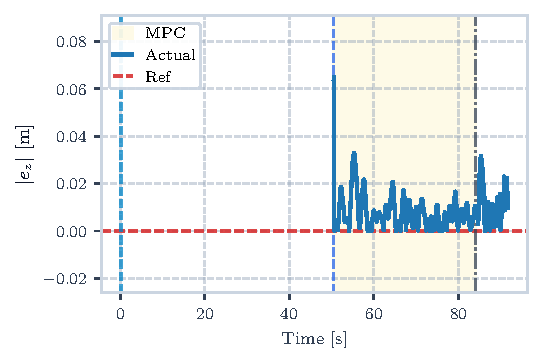
\includegraphics[width=\linewidth]{Immagini/Capitolo6/Simulations/Hovering/CYL_POV_ERR_elevation_error_z_err.pdf}
    \label{fig:placeholder}
\end{subfigure}
\begin{subfigure}[b]{0.49\textwidth}
    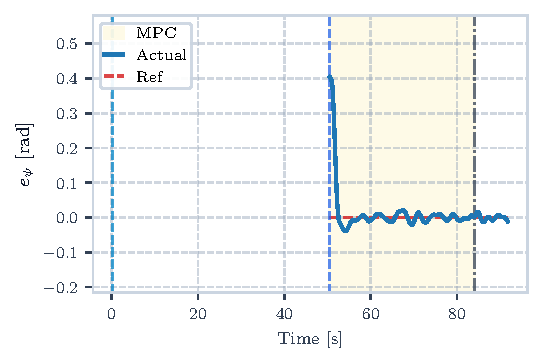
\includegraphics[width=\linewidth]{Immagini/Capitolo6/Simulations/Hovering/YAW_yaw_error.pdf}
    \label{fig:placeholder}
\end{subfigure}
\caption{Error norms - Cylindrical position and yaw orientation}
\label{fig:hovering_err}
\end{figure}
\\The observer drone pose shown in \ref{fig:hovering_pos} is computed based on visual references, that are cylindrical ones. For this reason figure \ref{fig:hovering_err} shows cylindrical errors, minimized in the NMPC cost function.
\begin{figure}[h!]
\centering
\begin{subfigure}[b]{0.51\textwidth}
    
\includegraphics[width=\linewidth]{Immagini/Capitolo6/Simulations/Hovering/phases_legend.pdf}
\end{subfigure}
\begin{subfigure}[b]{0.49\textwidth}
    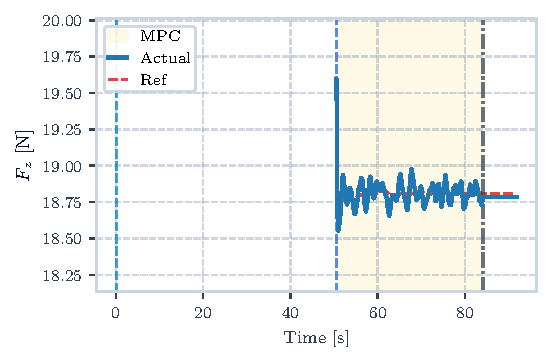
\includegraphics[width=\linewidth]{Immagini/Capitolo6/Simulations/Hovering/CONTROL_WRENCH_force_z.pdf}
    \label{fig:placeholder}
\end{subfigure}
\begin{subfigure}[b]{0.49\textwidth}
    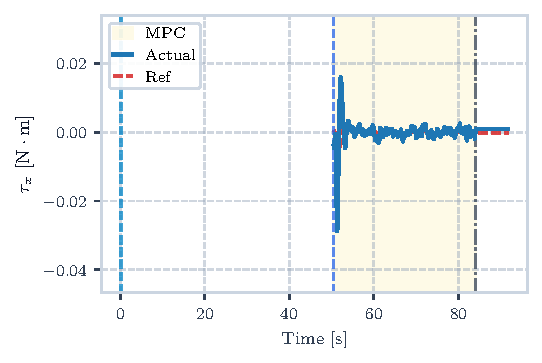
\includegraphics[width=\linewidth]{Immagini/Capitolo6/Simulations/Hovering/CONTROL_WRENCH_torque_x.pdf}
    \label{fig:placeholder}
\end{subfigure}
\begin{subfigure}[b]{0.49\textwidth}
    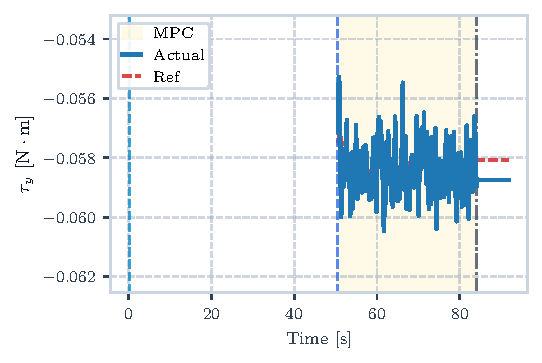
\includegraphics[width=\linewidth]{Immagini/Capitolo6/Simulations/Hovering/CONTROL_WRENCH_torque_y.pdf}
    \label{fig:placeholder}
\end{subfigure}
\begin{subfigure}[b]{0.49\textwidth}
    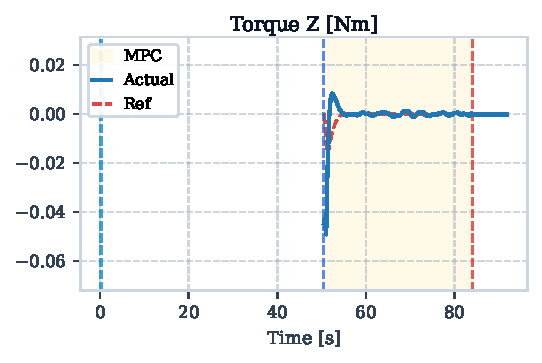
\includegraphics[width=\linewidth]{Immagini/Capitolo6/Simulations/Hovering/CONTROL_WRENCH_torque_z.pdf}
    \label{fig:placeholder}
\end{subfigure}
\caption{Hovering - Control wrench}
\label{fig:control_switch}
\end{figure}
Figure \ref{fig:control_switch} illustrates the body thrust and torques during the switch phase. Also thanks to the safety check over Euclidean distance between the PID-computed outputs and the NMPC-predicted outputs, so that it falls below the safety threshold $\epsilon$, the control signals remain perfectly continuous. This result is very important, since one of the main objective of the MPC controller was to consider actuation constraints inside the problem and thrust and torques are the real outputs of this controller. \\It is worth to notice that control torque $\tau_y$ oscillates around a value different from 0. This is due to model mismatches, precisely to a camera umodeled displacement with respect to CoM. This doesn't represent a problem, anyway, since both this and other disturbances can be handled by the MBE (\ref{fig:MBE}) that, regardless, brings tracking errors to 0.
\begin{figure}[h!]
\centering
\begin{subfigure}[b]{0.71\textwidth}
    
\includegraphics[width=\linewidth]{Immagini/Capitolo6/Simulations/Hovering/phases_legend.pdf}
\end{subfigure}
\begin{subfigure}[b]{0.32\textwidth}
    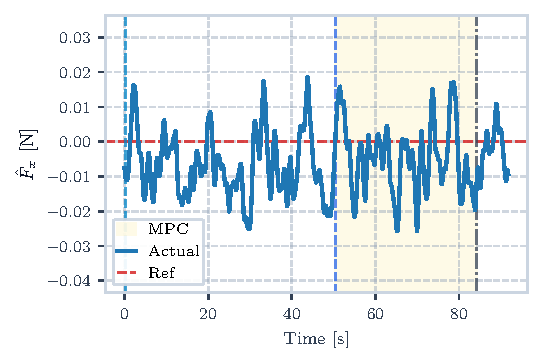
\includegraphics[width=\linewidth]{Immagini/Capitolo6/Simulations/Hovering/MBE_force_x.pdf}
    \label{fig:placeholder}
\end{subfigure}
\begin{subfigure}[b]{0.32\textwidth}
    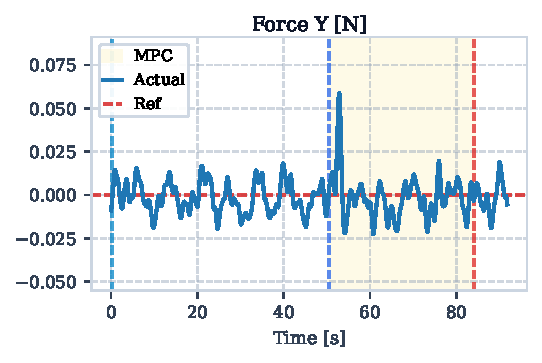
\includegraphics[width=\linewidth]{Immagini/Capitolo6/Simulations/Hovering/MBE_force_y.pdf}
    \label{fig:placeholder}
\end{subfigure}
\begin{subfigure}[b]{0.32\textwidth}
    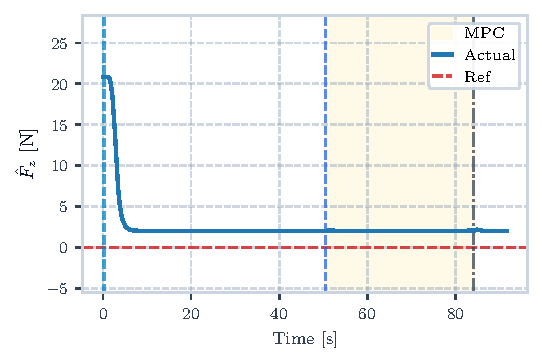
\includegraphics[width=\linewidth]{Immagini/Capitolo6/Simulations/Hovering/MBE_force_z.pdf}
    \label{fig:placeholder}
\end{subfigure}
\begin{subfigure}[b]{0.32\textwidth}
    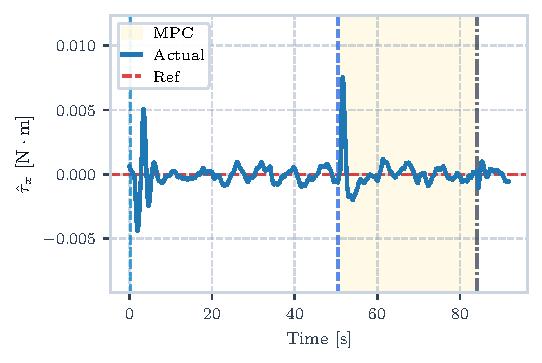
\includegraphics[width=\linewidth]{Immagini/Capitolo6/Simulations/Hovering/MBE_torque_x.pdf}
    \label{fig:placeholder}
\end{subfigure}
\begin{subfigure}[b]{0.32\textwidth}
    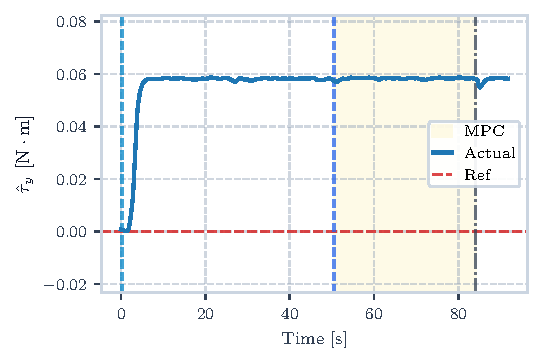
\includegraphics[width=\linewidth]{Immagini/Capitolo6/Simulations/Hovering/MBE_torque_y.pdf}
    \label{fig:placeholder}
\end{subfigure}
\begin{subfigure}[b]{0.32\textwidth}
    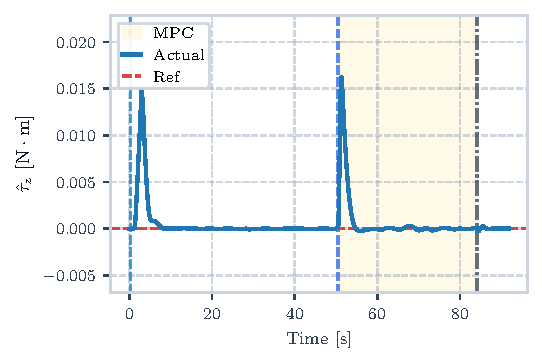
\includegraphics[width=\linewidth]{Immagini/Capitolo6/Simulations/Hovering/MBE_torque_z.pdf}
    \label{fig:placeholder}
\end{subfigure}
\caption{Hovering - Momentum Based Estimator, external estimated wrenches}
\label{fig:MBE}
\end{figure}

\subsection{Computational Efficiency}
Real-time feasibility is a strict requirement for aerial optimal control. A statistical analysis of the solver's execution time over the entire flight log confirms the extreme efficiency of the C-generated Acados code. 
\begin{figure}[h!]
\centering
\begin{subfigure}[b]{0.51\textwidth}
    
\includegraphics[width=\linewidth]{Immagini/Capitolo6/Simulations/Hovering/phases_legend.pdf}
\end{subfigure}
\begin{subfigure}[b]{0.8\textwidth}
    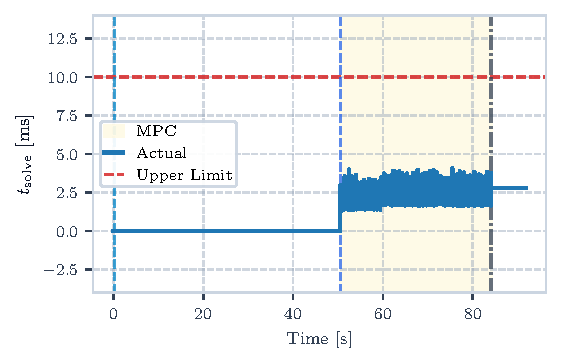
\includegraphics[width=\linewidth]{Immagini/Capitolo6/Simulations/Hovering/SOLVE_TIME_solve_time.pdf}
    \label{fig:placeholder}
\end{subfigure}
\caption{Hovering - NMPC Solving time}
\label{fig:solve_time}
\end{figure}
The NMPC cycle recorded an average execution time of $2.20$ ms, with a worst-case peak of $4.07$ ms. Since the solver must complete its routine within the $10$ ms discretization window ($T_s$), the system achieved a $0\%$ overrun rate. This is an important result for safely bringing the architecture over the onboard companion computer.

\section{Haptic Bilateral Teleoperation}
Having validated the baseline hovering stability of the NMPC, the second testing phase isolates and evaluates the human-machine interface. The objective is to demonstrate how the human operator can dynamically alter the Observer Drone's Point of View (PoV) via the Novint Falcon, and how the system safely handles conflicting inputs through force feedback.
\\During this test, the human operator uses the haptic device to command continuous variations of the cylindrical references: radial distance ($\rho_{ref}$), relative angular azimuth ($\beta_{ref}$), and relative height ($z_{ref}$).
\begin{figure}[h!]
\centering
\begin{subfigure}[b]{0.51\textwidth}
    
\includegraphics[width=\linewidth]{Immagini/Capitolo6/Simulations/Haptic/phases_legend.pdf}
\end{subfigure}
\begin{subfigure}[b]{0.49\textwidth}
    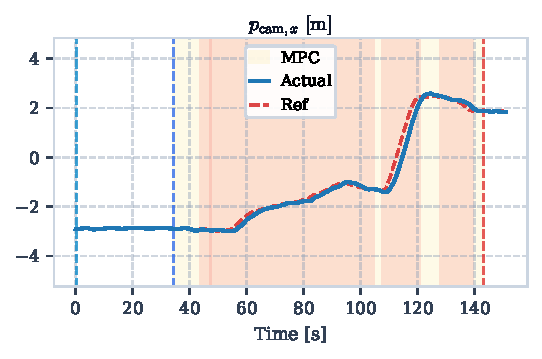
\includegraphics[width=\linewidth]{Immagini/Capitolo6/Simulations/Haptic/POS_cam_x.pdf}
    \label{fig:placeholder}
\end{subfigure}
\begin{subfigure}[b]{0.49\textwidth}
    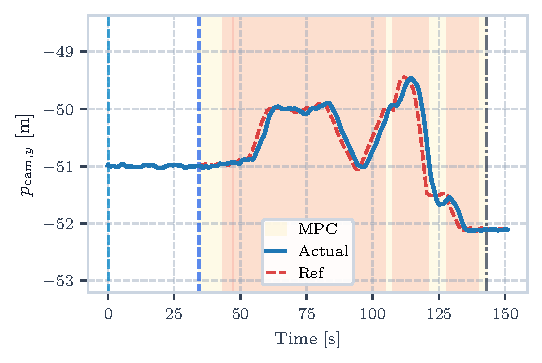
\includegraphics[width=\linewidth]{Immagini/Capitolo6/Simulations/Haptic/POS_cam_y.pdf}
    \label{fig:placeholder}
\end{subfigure}
\begin{subfigure}[b]{0.49\textwidth}
    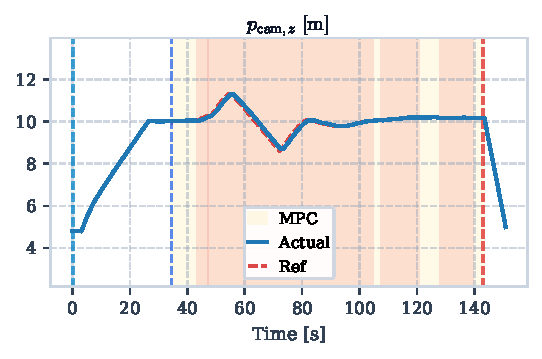
\includegraphics[width=\linewidth]{Immagini/Capitolo6/Simulations/Haptic/POS_cam_z.pdf}
    \label{fig:placeholder}
\end{subfigure}
\begin{subfigure}[b]{0.49\textwidth}
    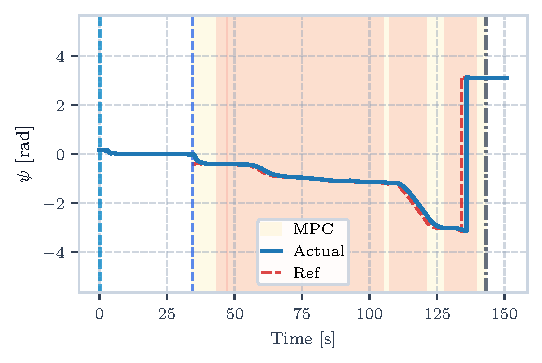
\includegraphics[width=\linewidth]{Immagini/Capitolo6/Simulations/Haptic/YAW_yaw.pdf}
    \label{fig:placeholder}
\end{subfigure}
\caption{Cartesian coordinates of Observer Drone camera in ENU frame}
\label{fig:haptic_pos}
\end{figure}
Figure \ref{fig:haptic_pos} shows the UAV's response to dynamic haptic commands.
The NMPC shows to be capable of tracking time-varying setpoints, smoothly adapting the drone's spatial position consistently with operator's intent. The mean errors across all cylindrical coordinates remain within acceptable operational margins, highlighting the absence of phase lags despite the complexity of the nonlinear optimization, as it is shown by figure \ref{fig:haptic_cyl}. There's some delay, anyway, as but it is simply due to MPC gains choice: penalizing acceleration, jerk and snap makes the flight smoother but also a bit less reactive. 
\begin{figure}[h!]
\centering
\begin{subfigure}[b]{0.51\textwidth}
    
\includegraphics[width=\linewidth]{Immagini/Capitolo6/Simulations/Haptic/phases_legend.pdf}
\end{subfigure}
\begin{subfigure}[b]{0.49\textwidth}
    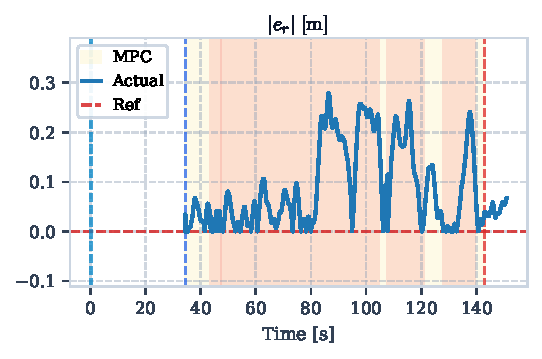
\includegraphics[width=\linewidth]{Immagini/Capitolo6/Simulations/Haptic/CYL_POV_ERR_distance_error_r_cyl_err.pdf}
    \label{fig:placeholder}
\end{subfigure}
\begin{subfigure}[b]{0.49\textwidth}
    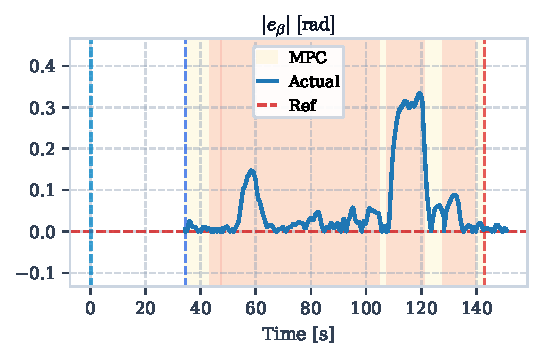
\includegraphics[width=\linewidth]{Immagini/Capitolo6/Simulations/Haptic/CYL_POV_ERR_azimuth_error_beta_err.pdf}
    \label{fig:placeholder}
\end{subfigure}
\begin{subfigure}[b]{0.49\textwidth}
    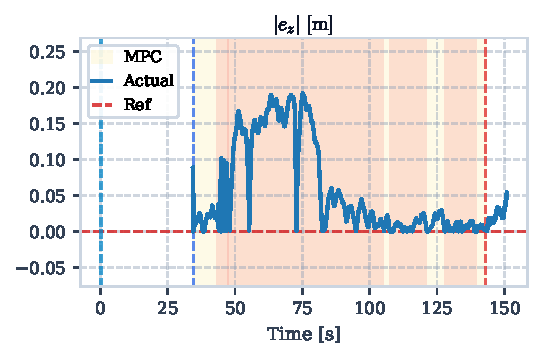
\includegraphics[width=\linewidth]{Immagini/Capitolo6/Simulations/Haptic/CYL_POV_ERR_elevation_error_z_err.pdf}
    \label{fig:placeholder}
\end{subfigure}
\begin{subfigure}[b]{0.49\textwidth}
    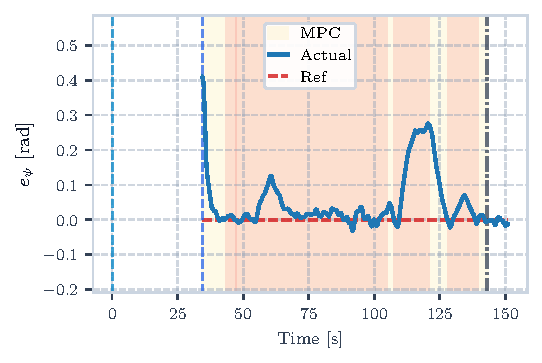
\includegraphics[width=\linewidth]{Immagini/Capitolo6/Simulations/Haptic/YAW_yaw_error.pdf}
    \label{fig:placeholder}
\end{subfigure}
\caption{Errors on cylindrical variables and yaw orientation}
\label{fig:haptic_cyl}
\end{figure}
\\However, human teleoperation commands can be unpredictable and may lead the vehicle towards unfeasible or unsafe configurations, such as bringing the Observer dangerously close to the target or causing visual loss by pushing the target outside the camera Field of View (FOV). To evaluate the Artificial Potential Field (APF) virtual fixtures, the operator deliberately commanded the drone towards the safety boundaries.

Figures~\ref{fig:APF_violations_sim} and~\ref{fig:APF_forces_sim} illustrate the resulting constraint violations and the corresponding repulsive forces rendered by the haptic device during the simulation.
\begin{figure}[h!]
\centering
\begin{subfigure}[b]{0.71\textwidth}
    
\includegraphics[width=\linewidth]{Immagini/Capitolo6/Simulations/Haptic/phases_legend.pdf}
\end{subfigure}
\begin{subfigure}[b]{0.32\textwidth}
    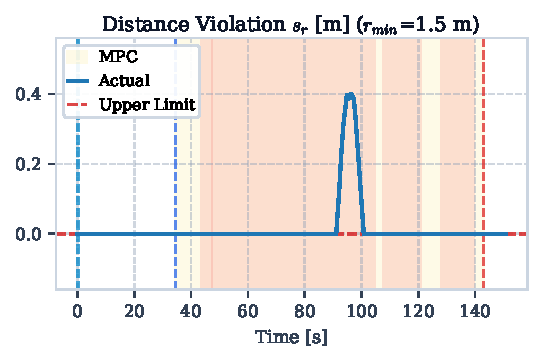
\includegraphics[width=\linewidth]{Immagini/Capitolo6/Simulations/Haptic/APF_distance_violation_s_r.pdf}
    \caption{Distance violation $s_r$}
\end{subfigure}
\begin{subfigure}[b]{0.32\textwidth}
    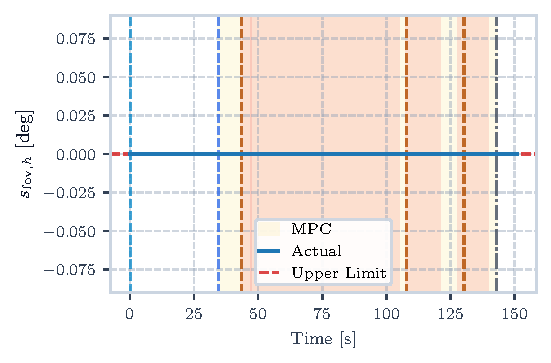
\includegraphics[width=\linewidth]{Immagini/Capitolo6/Simulations/Haptic/APF_horiz_fov_violation_s__fov_h.pdf}
    \caption{Horizontal FoV violation $s_{fov,h}$}
\end{subfigure}
\begin{subfigure}[b]{0.32\textwidth}
    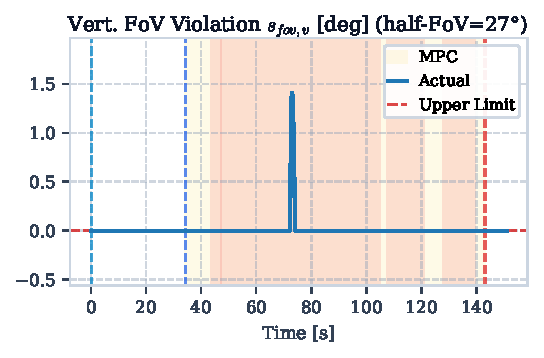
\includegraphics[width=\linewidth]{Immagini/Capitolo6/Simulations/Haptic/APF_vert_fov_violation_s__fov_v.pdf}
    \caption{Vertical FoV violation $s_{fov,v}$}
\end{subfigure}
\caption{Artificial Potential Field boundary violations during simulated haptic teleoperation}
\label{fig:APF_violations_sim}
\end{figure}

\begin{figure}[h!]
\centering
\begin{subfigure}[b]{0.71\textwidth}
    
\includegraphics[width=\linewidth]{Immagini/Capitolo6/Simulations/Haptic/phases_legend.pdf}
\end{subfigure}
\begin{subfigure}[b]{0.32\textwidth}
    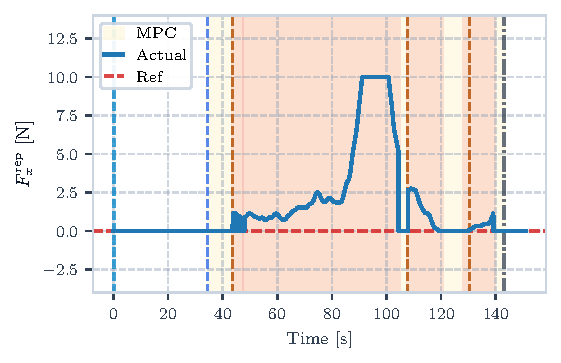
\includegraphics[width=\linewidth]{Immagini/Capitolo6/Simulations/Haptic/REPULSIVE_FORCES_repulsive_force_x.pdf}
    \caption{Radial repulsive force $F_x^{\text{rep}}$}
\end{subfigure}
\begin{subfigure}[b]{0.32\textwidth}
    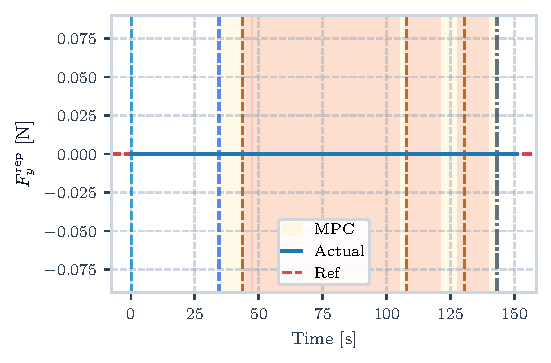
\includegraphics[width=\linewidth]{Immagini/Capitolo6/Simulations/Haptic/REPULSIVE_FORCES_repulsive_force_y.pdf}
    \caption{Azimuth repulsive force $F_y^{\text{rep}}$}
\end{subfigure}
\begin{subfigure}[b]{0.32\textwidth}
    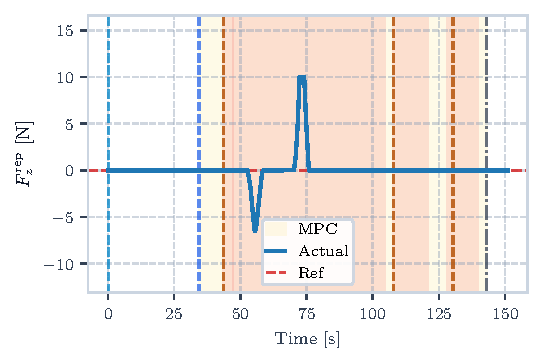
\includegraphics[width=\linewidth]{Immagini/Capitolo6/Simulations/Haptic/REPULSIVE_FORCES_repulsive_force_z.pdf}
    \caption{Elevation repulsive force $F_z^{\text{rep}}$}
\end{subfigure}
\caption{Repulsive forces rendered to the human operator via the haptic interface during simulated teleoperation}
\label{fig:APF_forces_sim}
\end{figure}

As shown in the plots, the system reliably reacts to the impending hazards:
\begin{itemize}
    \item \textbf{Radial Distance Violation ($s_r$):} Around $t \approx 91\text{ s}$, the pilot pushes the joystick forward, commanding an aggressive approach towards the Inspection UAV. As the standoff distance breaches the safety threshold $r_{\min} = 1.50\text{ m}$, the exponential repulsive force $F_x^{\text{rep}}$ rises sharply and reaches the saturation threshold of $10.0\text{ N}$ (from $t \approx 91.1\text{ s}$). The maximum encroachment reaches $s_r = 0.40\text{ m}$ at $t = 96.15\text{ s}$, meaning the inter-drone distance momentarily dropped to $r_{\text{cyl}} = 1.10\text{ m}$ (a $40\text{ cm}$ safety encroachment). The persistent tactile resistance alerts the operator to the collision hazard, prompting them to release forward pressure. As a consequence, the standoff distance smoothly recovers beyond $1.50\text{ m}$ at $t = 100.65\text{ s}$, and $s_r$ promptly returns to zero.
    \item \textbf{Vertical FoV Violation ($s_{\text{fov},v}$):} Around $t \approx 72\text{ s}$, the operator commands an upward climb, raising the Observer's altitude relative to the target. Because the camera has a fixed pitch, the target approaches the bottom boundary of the vertical Field of View ($\text{FOV}_v = 54.5^\circ$, semi-aperture $\approx 27.3^\circ$). At $t = 73.03\text{ s}$, a transient angular violation of $s_{\text{fov},v} = 1.41^\circ$ ($0.025\text{ rad}$) is recorded. Geometrically, at the current standoff distance of $r_{\text{cyl}} = 2.40\text{ m}$, the optical semi-aperture corresponds to a maximum visible semi-height of $z_{\max} = 1.24\text{ m}$, whereas the drone reached $|z_{\text{cyl}}| = 1.31\text{ m}$. This corresponds to a physical height overshoot of:
    \begin{equation}
        \Delta z = |z_{\text{cyl}}| - z_{\max} = 1.31\text{ m} - 1.24\text{ m} = 7.57\text{ cm}.
    \end{equation}
    The target thus exceeded the optical boundary by only $\approx 7.6\text{ cm}$. In response, the APF instantly delivers a downward repulsive force $F_z^{\text{rep}} = -10.0\text{ N}$ to the joystick handle. This prompt tactile cue guides the pilot to descend, recovering visual framing within just $1.8\text{ s}$ ($t = 74.09\text{ s}$).
    \item \textbf{Horizontal FoV ($s_{\text{fov},h}$):} Throughout the entire teleoperation session, the horizontal FOV violation remains strictly zero ($s_{\text{fov},h} = 0.00^\circ$, $F_y^{\text{rep}} = 0.0\text{ N}$). This confirms that the autonomous yaw tracking loop maintains the optical axis tightly aligned with the target's relative azimuth, absorbing the lateral dynamics and preventing target loss on the horizontal image plane.
\end{itemize}

\section{Complete Cooperative Mission (SITL)}
The final stage of the Software-in-the-Loop validation integrates all modules into the full dual-drone cooperative architecture. In this scenario, the Inspection Drone executes a programmed approach toward a structure, while the Observer Drone autonomously maintains the visual, guided by the NMPC and the operator's haptic supervision.
\\Moreover, the mission is planned to autonomously change visual parameters $r,\beta,z_{rel},\psi$ at each phase of the mission, according to phase visual requirements, in order to help the operator in supervising the mission itself and to teleoperate the other drone at the best of his capabilities.
\begin{figure}[h!]
    \centering
    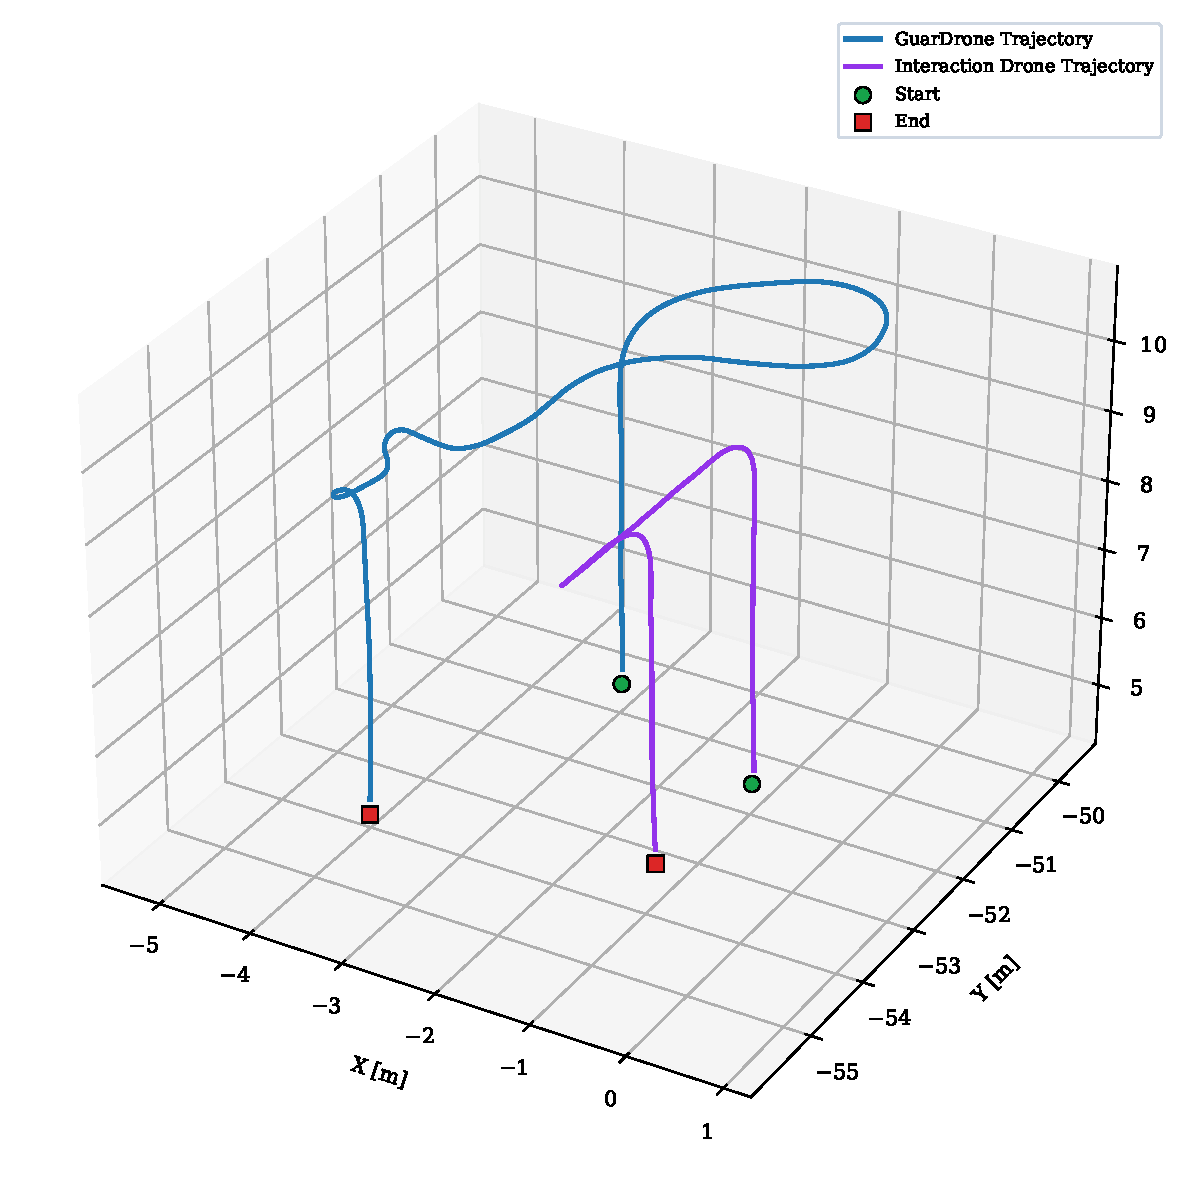
\includegraphics[width=0.5\linewidth]{Immagini/Capitolo6/Simulations/Mission/3D.pdf}
    \caption{3D trajectories of the two drones}
    \label{fig:3d_mission}
\end{figure}
The spatial evolution of the mission is captured in the 3D trajectory plot (Figure \ref{fig:3d_mission}) and in the respective Cartesian coordinates (Figures \ref{fig:mission_cam_pose} and \ref{fig:mission_int_pose}). The mission evolves through sequential operational phases governed by the FSM, depicted in Figure \ref{fig:sim_mission_phases}:

\begin{figure}[htbp]
\centering
\begin{subfigure}[b]{0.48\textwidth}
    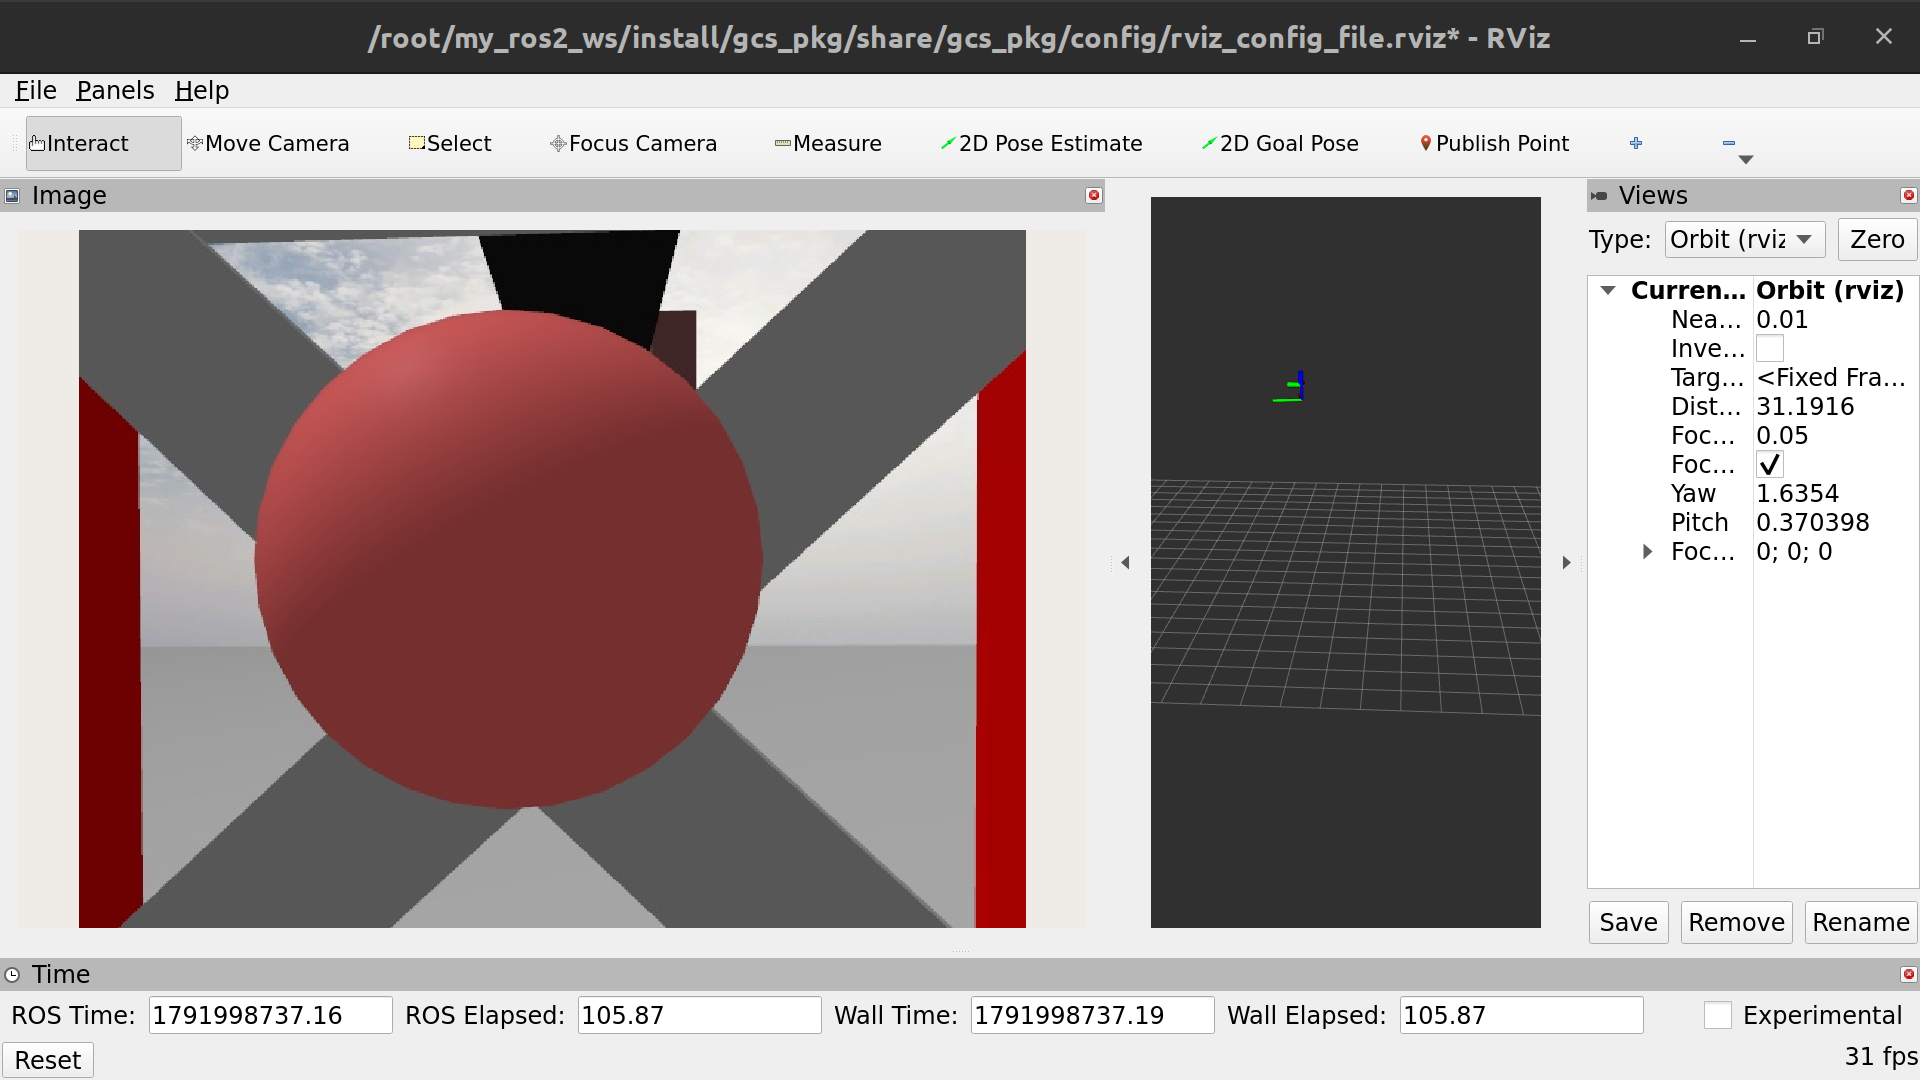
\includegraphics[width=\linewidth]{Immagini/Capitolo6/Simulations/PHASES/phase_obstacle.png}
    \caption{Navigation \& obstacle avoidance via teleoperation}
    \label{fig:sim_phase_obstacle}
\end{subfigure}
\hfill
\begin{subfigure}[b]{0.48\textwidth}
    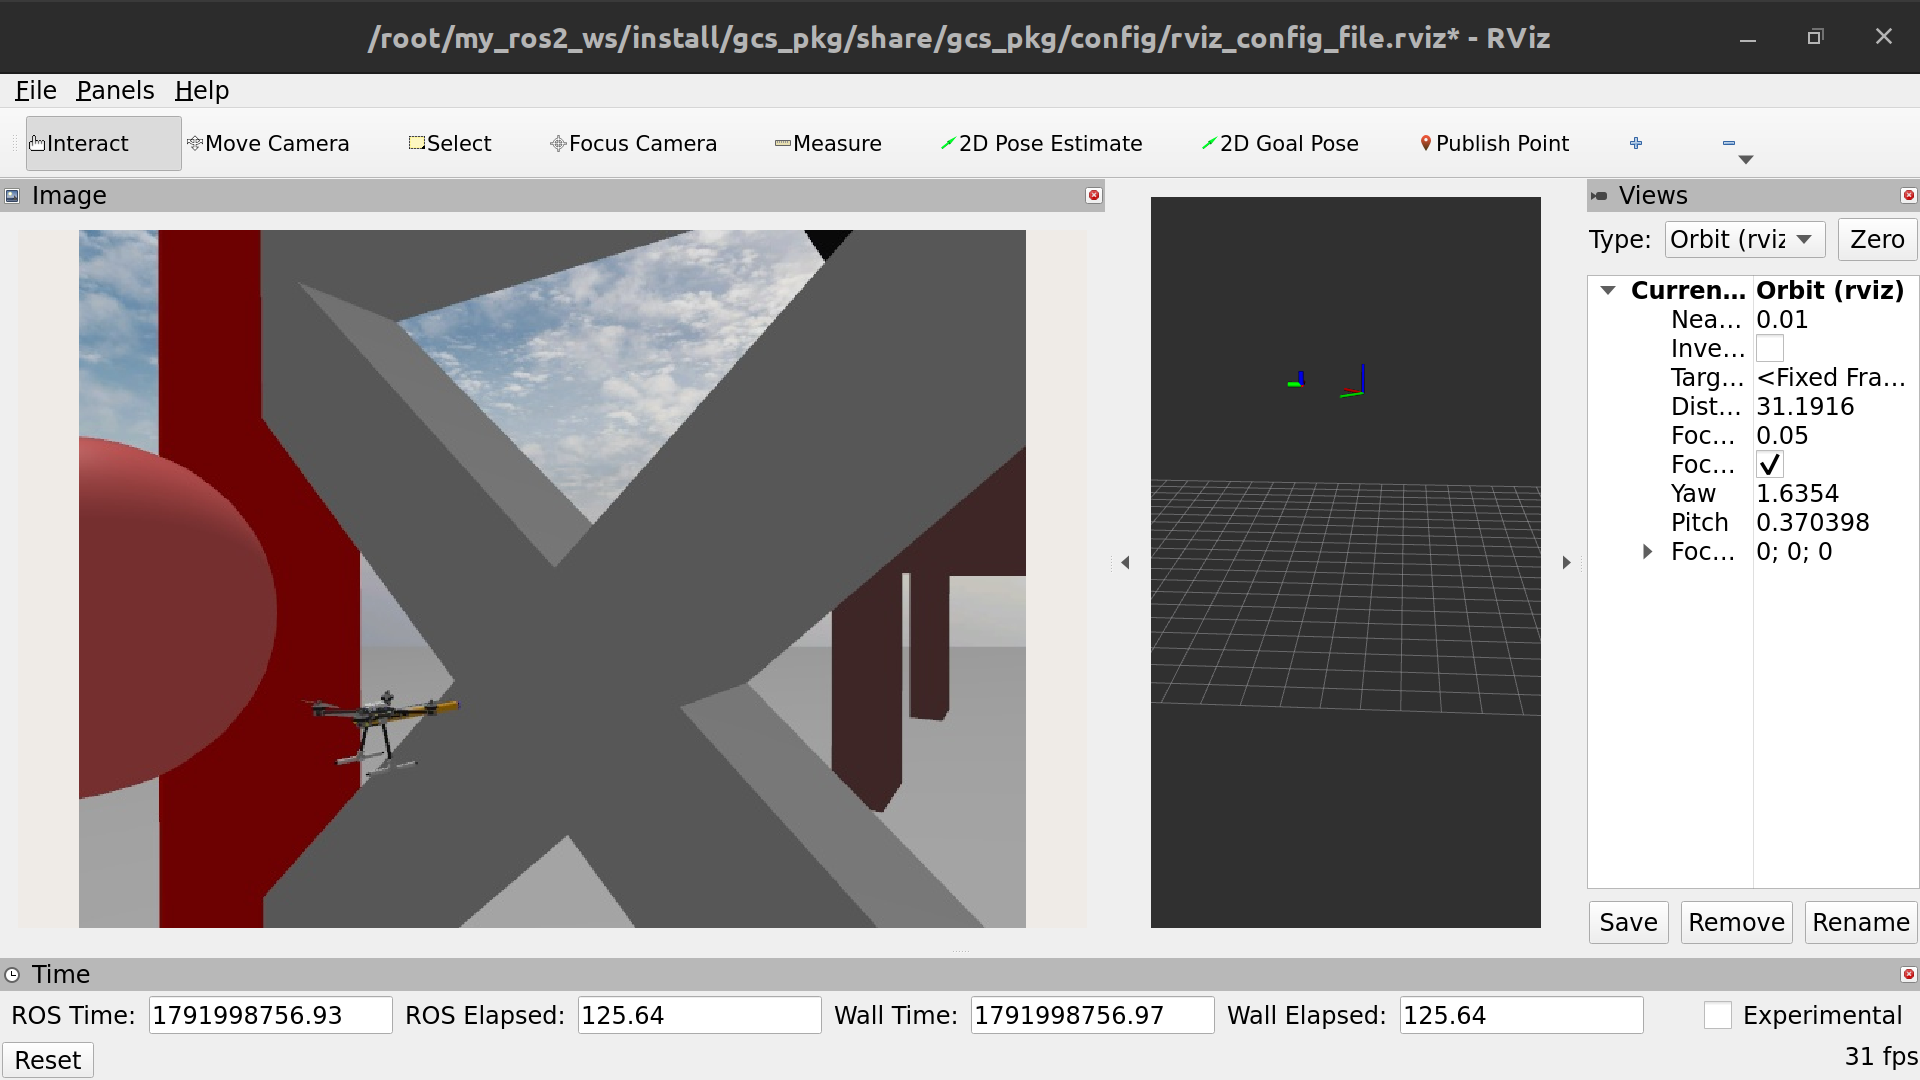
\includegraphics[width=\linewidth]{Immagini/Capitolo6/Simulations/PHASES/phase_approach.png}
    \caption{Autonomous approach toward target structure}
    \label{fig:sim_phase_approach}
\end{subfigure}
\\[1.5ex]
\begin{subfigure}[b]{0.48\textwidth}
    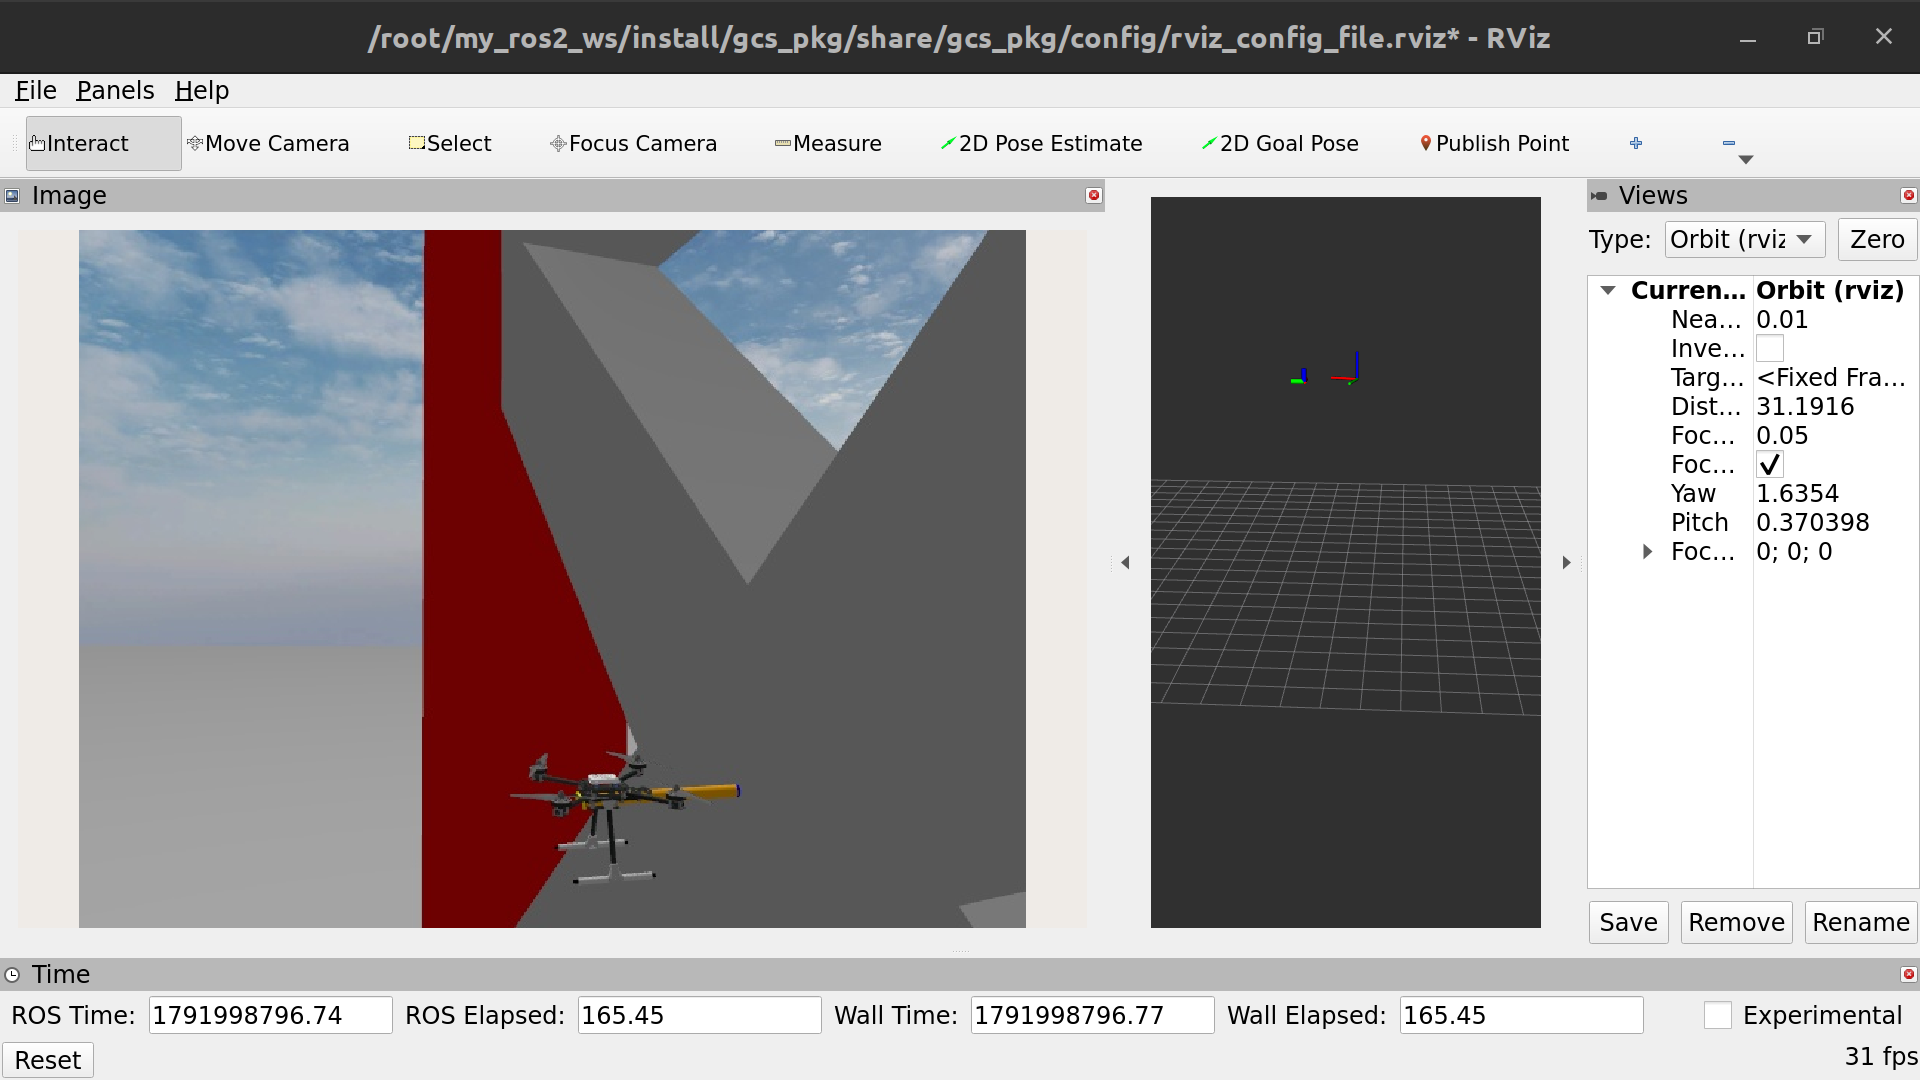
\includegraphics[width=\linewidth]{Immagini/Capitolo6/Simulations/PHASES/phase_interaction.png}
    \caption{Compliant physical contact and decoupled framing}
    \label{fig:sim_phase_interaction}
\end{subfigure}
\hfill
\begin{subfigure}[b]{0.48\textwidth}
    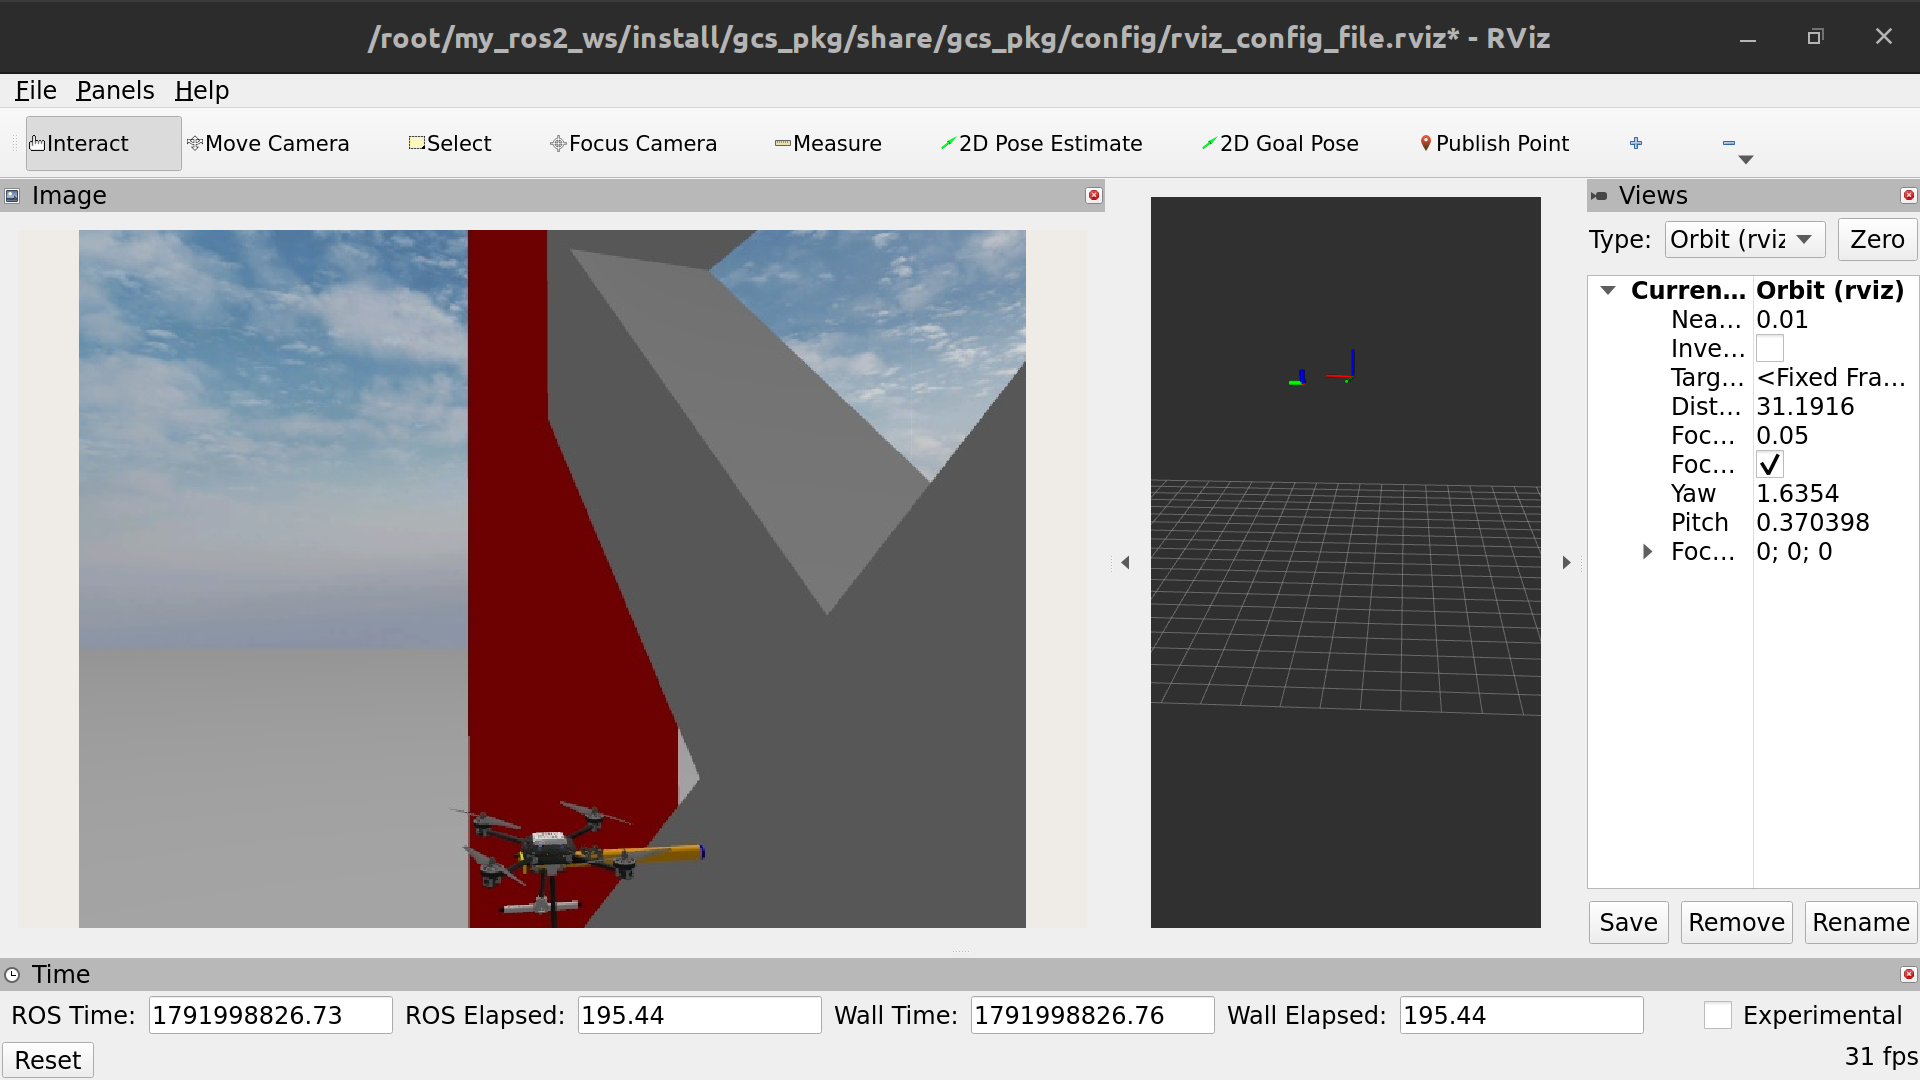
\includegraphics[width=\linewidth]{Immagini/Capitolo6/Simulations/PHASES/phase_detachment.png}
    \caption{Safe vehicle detachment}
    \label{fig:sim_phase_detachment}
\end{subfigure}
\\[1.5ex]
\begin{subfigure}[b]{0.50\textwidth}
    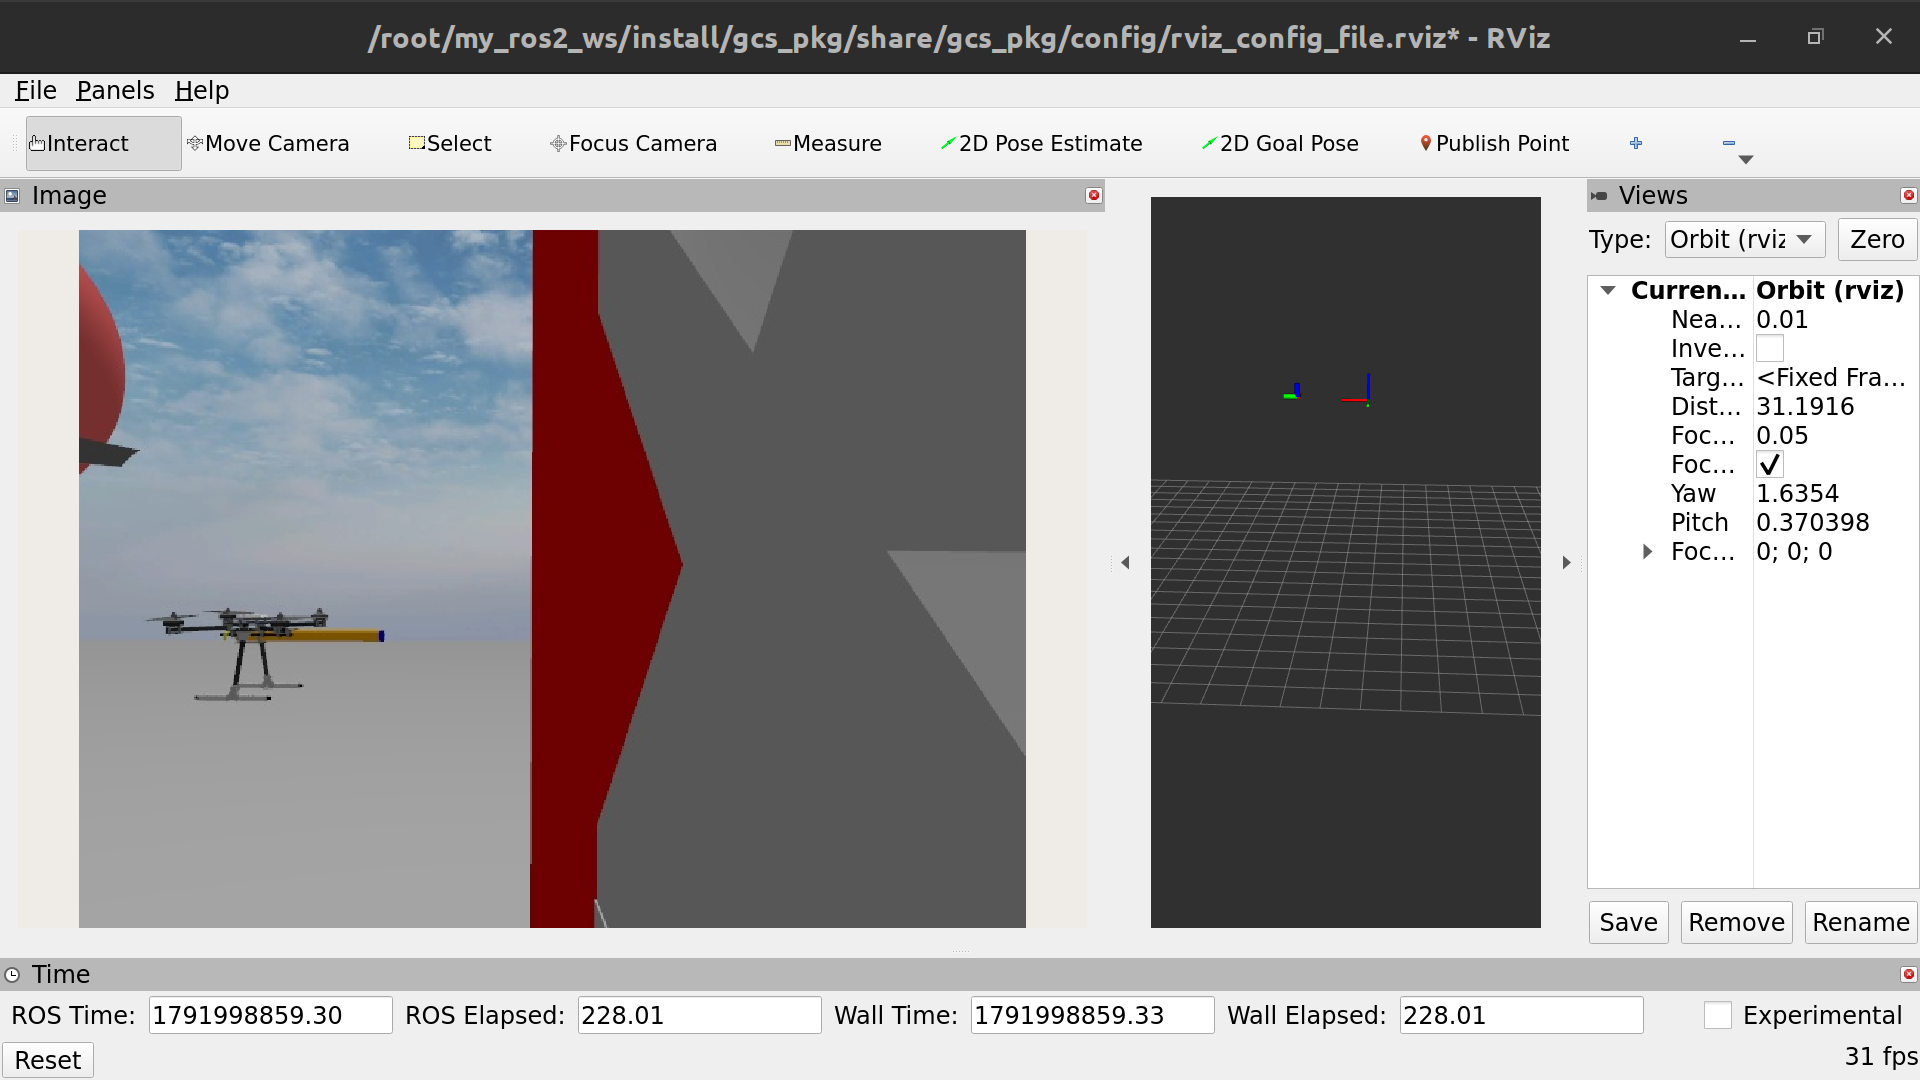
\includegraphics[width=\linewidth]{Immagini/Capitolo6/Simulations/PHASES/phase_return_home.png}
    \caption{Autonomous return-to-home navigation}
    \label{fig:sim_phase_return_home}
\end{subfigure}
\caption{Gazebo simulation snapshots illustrating the sequential operational phases of the cooperative mission}
\label{fig:sim_mission_phases}
\end{figure}

\begin{itemize}
    \item \textbf{Takeoff \& Hovering Switch:} Both UAVs execute a vertical take-off using PX4 position control. Upon reaching hovering altitude, the Observer UAV switches to the NMPC controller, locking onto the Inspection UAV and maintaining the target centered in the image plane.
    \item \textbf{Navigation \& Obstacle Avoidance (Figure \ref{fig:sim_phase_obstacle}):} During the transit toward the inspection area, an unmodeled spherical obstacle (highlighted in red) is placed along the Observer's flight corridor. This demonstrates the key advantage of the shared teleoperation channel: the human pilot uses the haptic joystick to smoothly dodge the obstacle with intuitive lateral/vertical inputs, while the NMPC dynamically preserves visual tracking and distance constraints, preventing loss of visual contact.
    \item \textbf{Approach (Figure \ref{fig:sim_phase_approach}):} The Inspection Drone navigates toward the target structure, arresting its forward motion at a safe standoff distance of $2\text{ m}$ from the wall. The Observer tracks it autonomously, keeping a centered viewpoint at nominal standoff distance $r \approx 2.5\text{--}2.7\text{ m}$ to maximize depth perception.
    \item \textbf{Interaction (Figure \ref{fig:sim_phase_interaction}):} Upon operator authorization, the Inspection Drone pushes against the surface. The admittance control loop accommodates the contact force ($\simeq 2\text{ N}$ with compliant displacement of $\simeq 4\text{ cm}$). Simultaneously, the FSM commands an elevated viewpoint ($z_{rel} \approx 0.78\text{ m}$) with a yaw offset, shifting the target drone toward the bottom-right corner of the image plane so that the end-effector tip and the wall remain centered and unobstructed in the video stream.
    \item \textbf{Detachment (Figure \ref{fig:sim_phase_detachment}):} Once inspection is complete, the Inspection Drone retreats by $0.5\text{ m}$ from the wall. The Observer adjusts its vantage point ($r \approx 2.18\text{ m}$) to grant the operator clear visual feedback of the vehicle disengagement.
    \item \textbf{Return Home (Figure \ref{fig:sim_phase_return_home}):} The Inspection Drone navigates back to its initial take-off coordinates, while the Observer drone smoothly restores a centered visual perspective ($z_{rel} \to 0$, $r \approx 2.5\text{ m}$) until disarm and landing.
\end{itemize}
\begin{figure}[h!]
    \centering
    \begin{subfigure}[b]{0.71\textwidth}
        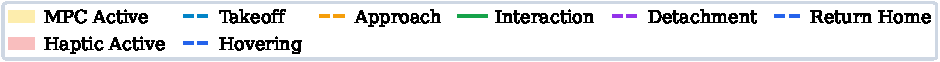
\includegraphics[width=\linewidth]{Immagini/Capitolo6/Simulations/Mission/phases_legend.pdf}
    \end{subfigure}
    \begin{subfigure}[b]{0.49\textwidth}
        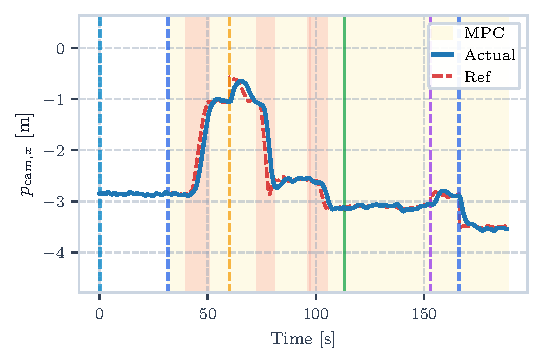
\includegraphics[width=\linewidth]{Immagini/Capitolo6/Simulations/Mission/POS_cam_x.pdf}
    \end{subfigure}
    \begin{subfigure}[b]{0.49\textwidth}
        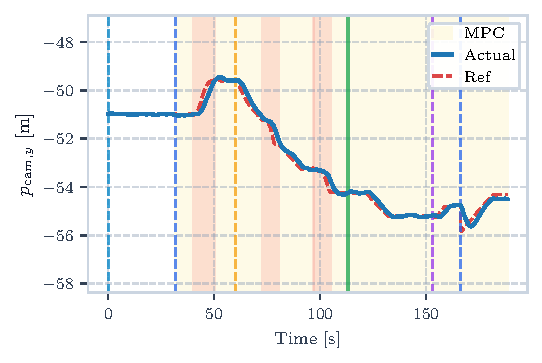
\includegraphics[width=\linewidth]{Immagini/Capitolo6/Simulations/Mission/POS_cam_y.pdf}
    \end{subfigure}
    \begin{subfigure}[b]{0.49\textwidth}
        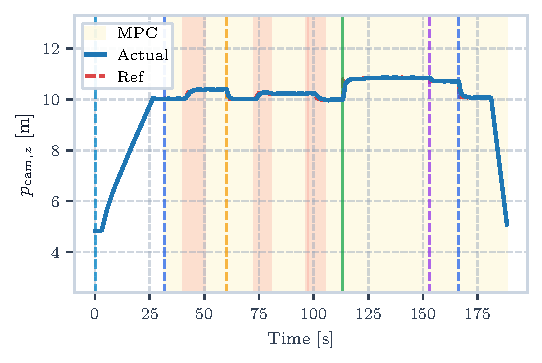
\includegraphics[width=\linewidth]{Immagini/Capitolo6/Simulations/Mission/POS_cam_z.pdf}
    \end{subfigure}
    \begin{subfigure}[b]{0.49\textwidth}
        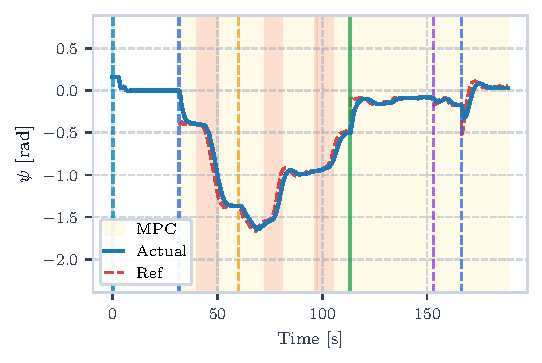
\includegraphics[width=\linewidth]{Immagini/Capitolo6/Simulations/Mission/YAW_yaw_actual_vs_desired.pdf}
    \end{subfigure}
    \caption{Position and orientation of the Observer Drone along the mission}
    \label{fig:mission_cam_pose}
\end{figure}
\begin{figure}[h!]
    \centering
    \begin{subfigure}[b]{0.71\textwidth}
        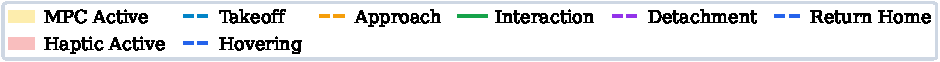
\includegraphics[width=\linewidth]{Immagini/Capitolo6/Simulations/Mission/phases_legend.pdf}
    \end{subfigure}
    \begin{subfigure}[b]{0.49\textwidth}
        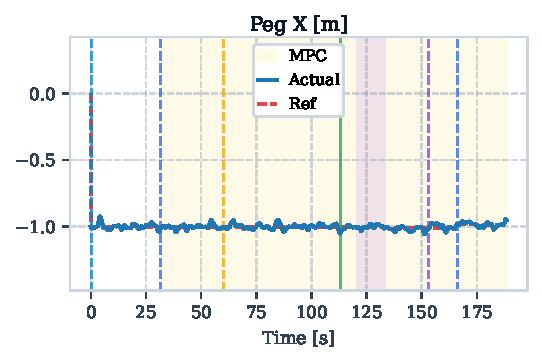
\includegraphics[width=\linewidth]{Immagini/Capitolo6/Simulations/Mission/INT_POS_peg_x.pdf}
    \end{subfigure}
    \begin{subfigure}[b]{0.49\textwidth}
        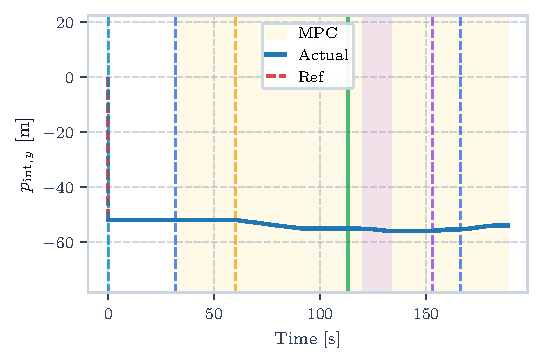
\includegraphics[width=\linewidth]{Immagini/Capitolo6/Simulations/Mission/INT_POS_peg_y.pdf}
    \end{subfigure}
    \begin{subfigure}[b]{0.49\textwidth}
        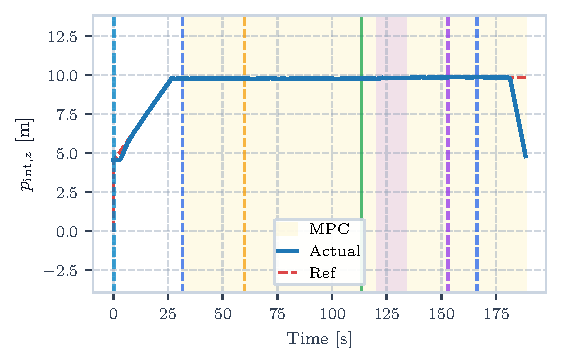
\includegraphics[width=\linewidth]{Immagini/Capitolo6/Simulations/Mission/INT_POS_peg_z.pdf}
    \end{subfigure}
    \begin{subfigure}[b]{0.49\textwidth}
        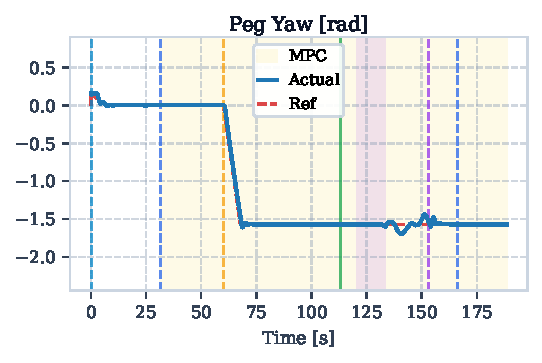
\includegraphics[width=\linewidth]{Immagini/Capitolo6/Simulations/Mission/INT_POS_peg_yaw.pdf}
    \end{subfigure}
    \caption{Position and orientation of the Interaction Drone along the mission}
    \label{fig:mission_int_pose}
\end{figure}
Figure \ref{fig:mission_cyl_pov} illustrates how the relative cylindrical variables are tracked across the mission and how relative setpoints adapt dynamically to each operational phase. During hovering and approach, the standoff distance is maintained around $r \approx 2.5\text{--}2.7\text{ m}$. During physical interaction, the reference adapts to $r_{\text{ref}} = 2.40\text{ m}$ to provide higher visual resolution of the contact interface, while the elevation offset increases to $z_{\text{rel}} \approx 0.78\text{ m}$ to frame the target vehicle in the lower corner of the field of view. During vehicle detachment, the radial distance contracts slightly to $r \approx 2.18\text{ m}$ to adapt the viewpoint before smoothly restoring the nominal distance $r \approx 2.50\text{ m}$ in the return-to-home phase.
\\Similarly, the elevation plot shows the autonomous offset introduced during interaction: by imposing an elevation displacement $z_{rel}$ and a corresponding yaw offset $\psi_{des}$, the target drone is deliberately shifted toward the bottom-right corner of the image plane. This ensures that the end-effector tip and the inspected wall remain fully visible and centered in the operator's FOV. The tracking errors across all cylindrical coordinates remain strictly bounded, proving that the NMPC smoothly handles the reference discontinuities commanded by the FSM without inducing aggressive transients or video shake.
\begin{figure}[h!]
\centering
\begin{subfigure}[b]{0.71\textwidth}
    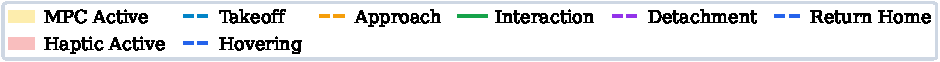
\includegraphics[width=\linewidth]{Immagini/Capitolo6/Simulations/Mission/phases_legend.pdf}
\end{subfigure}
\begin{subfigure}[b]{0.49\textwidth}
    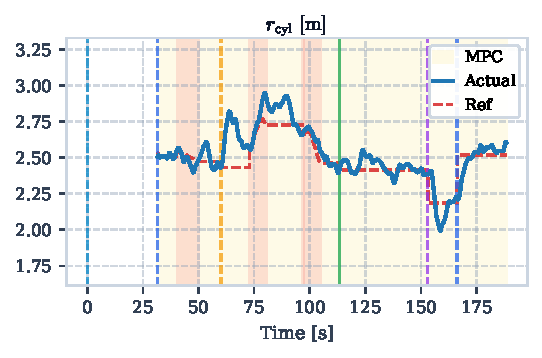
\includegraphics[width=\linewidth]{Immagini/Capitolo6/Simulations/Mission/CYL_POV_distance_r_cyl.pdf}
\end{subfigure}
\begin{subfigure}[b]{0.49\textwidth}
    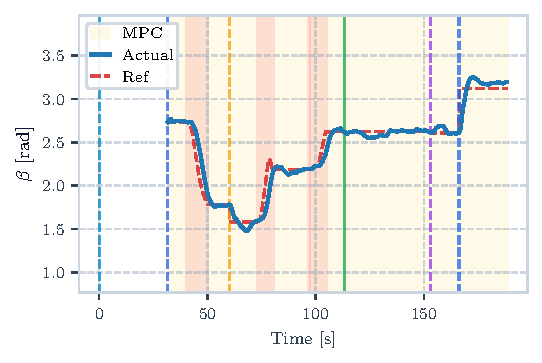
\includegraphics[width=\linewidth]{Immagini/Capitolo6/Simulations/Mission/CYL_POV_azimuth_beta.pdf}
\end{subfigure}
\begin{subfigure}[b]{0.49\textwidth}
    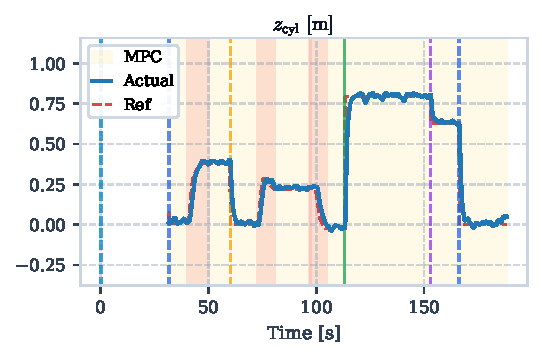
\includegraphics[width=\linewidth]{Immagini/Capitolo6/Simulations/Mission/CYL_POV_elevation_z.pdf}
\end{subfigure}
\begin{subfigure}[b]{0.49\textwidth}
    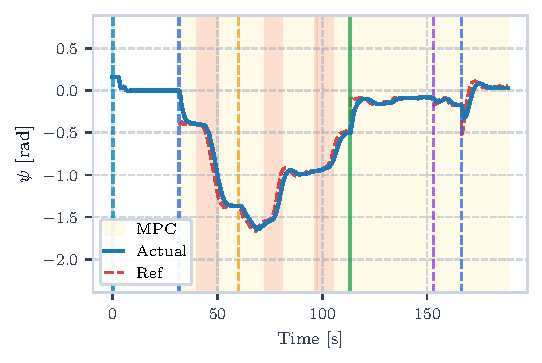
\includegraphics[width=\linewidth]{Immagini/Capitolo6/Simulations/Mission/YAW_yaw_actual_vs_desired.pdf}
\end{subfigure}
\caption{Cylindrical visual tracking variables along the cooperative mission}
\label{fig:mission_cyl_pov}
\end{figure}
To prevent visual fatigue and motion sickness for the operator, the NMPC formulation explicitly minimizes higher-order dynamic derivatives in the cost function. Figure \ref{fig:mission_derivative_norms} reports the Euclidean norms of linear acceleration, angular acceleration, jerk, and snap along the entire mission. 
\\As shown in the plots, all derivative norms remain smooth and bounded throughout the flight. Small variations occur only during phase transitions when adapting to new visual setpoints, but high-frequency jerk and snap are heavily damped. This validates that the camera motion remains remarkably fluid and free of sharp shakes, keeping the streamed video comfortable for human decision-making.
\begin{figure}[h!]
\centering
\begin{subfigure}[b]{0.71\textwidth}
    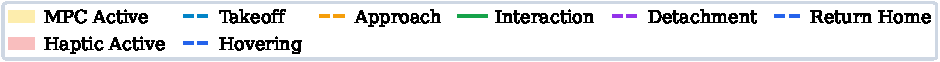
\includegraphics[width=\linewidth]{Immagini/Capitolo6/Simulations/Mission/phases_legend.pdf}
\end{subfigure}
\begin{subfigure}[b]{0.49\textwidth}
    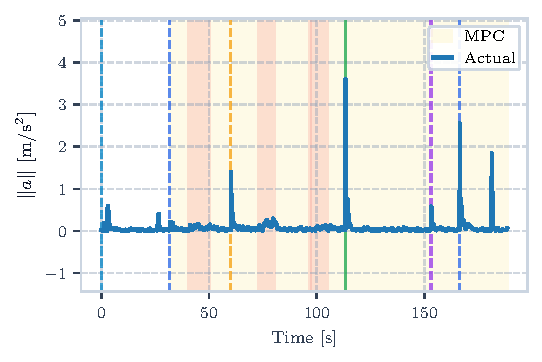
\includegraphics[width=\linewidth]{Immagini/Capitolo6/Simulations/Mission/DERIVATIVE_NORMS_norm_acc.pdf}
\end{subfigure}
\begin{subfigure}[b]{0.49\textwidth}
    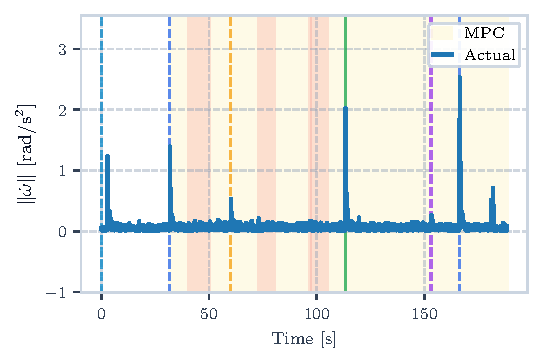
\includegraphics[width=\linewidth]{Immagini/Capitolo6/Simulations/Mission/DERIVATIVE_NORMS_norm_angacc.pdf}
\end{subfigure}
\begin{subfigure}[b]{0.49\textwidth}
    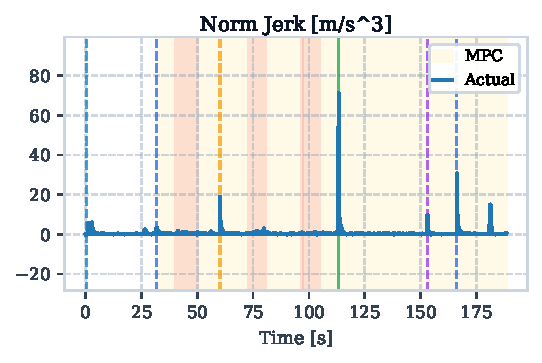
\includegraphics[width=\linewidth]{Immagini/Capitolo6/Simulations/Mission/DERIVATIVE_NORMS_norm_jerk.pdf}
\end{subfigure}
\begin{subfigure}[b]{0.49\textwidth}
    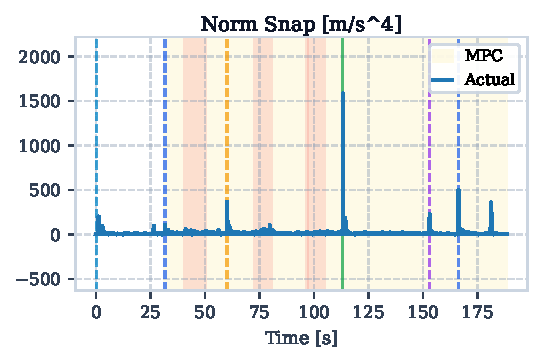
\includegraphics[width=\linewidth]{Immagini/Capitolo6/Simulations/Mission/DERIVATIVE_NORMS_norm_snap.pdf}
\end{subfigure}
\caption{Norms of higher-order dynamic derivatives penalised in the NMPC cost function during the mission}
\label{fig:mission_derivative_norms}
\end{figure}
Since the NMPC acts directly as a low-level dynamic controller, Figure \ref{fig:mission_control_wrench} illustrates the actual control wrench commanded to the Observer UAV. The total thrust $F_z$ stays around the nominal hovering weight ($\simeq 14.7\text{ N}$) without dangerous drops during the maneuvers. The commanded body torques ($\tau_x, \tau_y, \tau_z$) remain smooth and strictly inside the hard actuation bounds enforced by the solver ($[-U_\tau, U_\tau]$). Similar to the hovering test, $\tau_y$ compensates for the unmodeled camera offset without creating any instability, demonstrating the effectiveness of the online MBE feedforward.
\begin{figure}[h!]
\centering
\begin{subfigure}[b]{0.71\textwidth}
    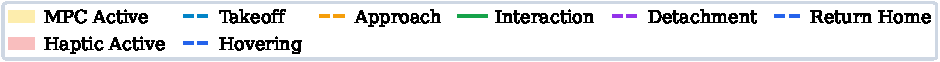
\includegraphics[width=\linewidth]{Immagini/Capitolo6/Simulations/Mission/phases_legend.pdf}
\end{subfigure}
\begin{subfigure}[b]{0.49\textwidth}
    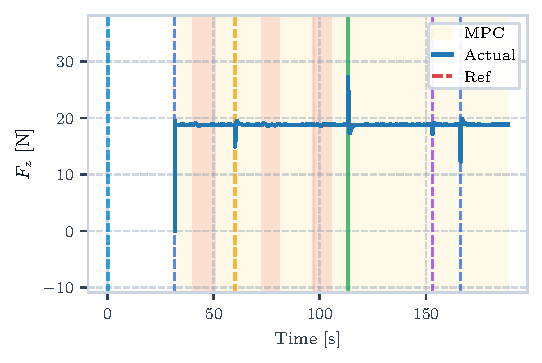
\includegraphics[width=\linewidth]{Immagini/Capitolo6/Simulations/Mission/CONTROL_WRENCH_force_z.pdf}
\end{subfigure}
\begin{subfigure}[b]{0.49\textwidth}
    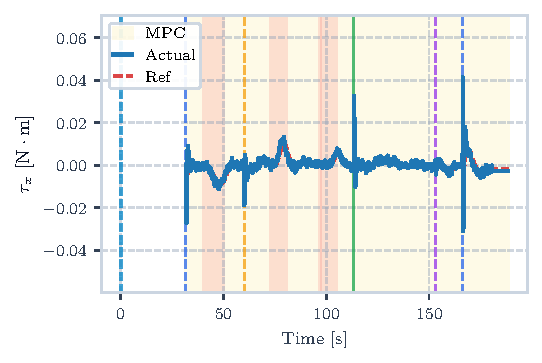
\includegraphics[width=\linewidth]{Immagini/Capitolo6/Simulations/Mission/CONTROL_WRENCH_torque_x.pdf}
\end{subfigure}
\begin{subfigure}[b]{0.49\textwidth}
    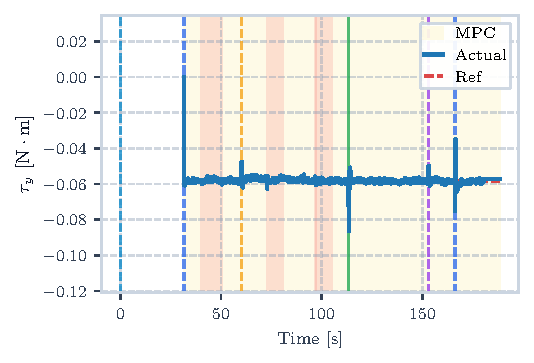
\includegraphics[width=\linewidth]{Immagini/Capitolo6/Simulations/Mission/CONTROL_WRENCH_torque_y.pdf}
\end{subfigure}
\begin{subfigure}[b]{0.49\textwidth}
    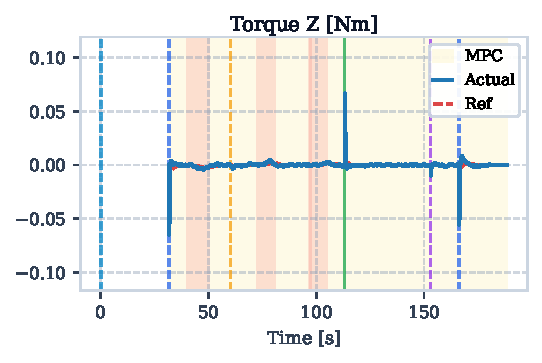
\includegraphics[width=\linewidth]{Immagini/Capitolo6/Simulations/Mission/CONTROL_WRENCH_torque_z.pdf}
\end{subfigure}
\caption{Control wrench commanded by the NMPC to the Observer UAV along the mission}
\label{fig:mission_control_wrench}
\end{figure}
A critical phase of this mission is the physical interaction with the environment. When the Inspection Drone touches the target surface, the tip-mounted virtual 1D force sensor detects the collision. 
\begin{figure}[h!]
    \centering
    \begin{subfigure}[b]{0.6\textwidth}
        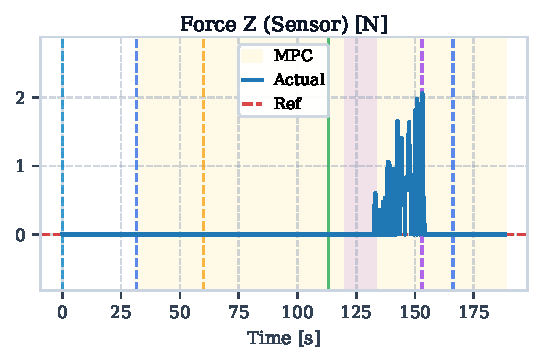
\includegraphics[width=\linewidth]{Immagini/Capitolo6/Simulations/Mission/SENSOR_FORCES_force_z.pdf}    
    \end{subfigure}
    \begin{subfigure}[b]{0.6\textwidth}
        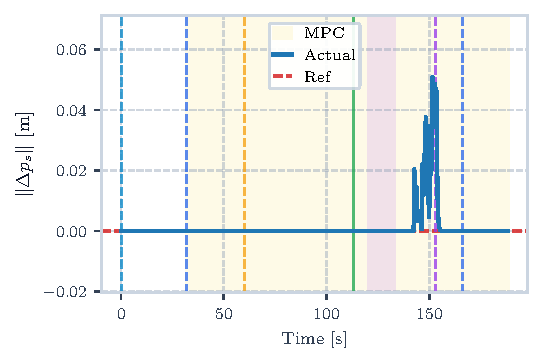
\includegraphics[width=\linewidth]{Immagini/Capitolo6/Simulations/Mission/INT_ADMITTANCE_SENSOR_p_s.pdf}
    \end{subfigure}
    \caption{Pre-filtered contact force and admittance displacement norm in sensor frame}
    \label{fig:admittance}
\end{figure}
As illustrated in Figure \ref{fig:admittance}, the raw contact forces are successfully filtered and processed by the admittance node. The bottom half of the plot highlights the deviation between the nominal, rigid trajectory and the compliant reference generated by the mass-damper-spring model given by admittance filter. Consequently, the Inspection Drone smoothly accommodates the external force, preventing mechanical damage and ensuring a safe and stable contact phase. A displacement of $\simeq4$cm is estimated by the filter, correspondent to $2$N external force.
\\Moreover, thanks to the dynamic behavior of the NMPC, the Observer Drone compensates for this sudden compliant shift of its target. The visual tracking remains robust throughout the entire interaction, validating the performance of the proposed multi-drone framework.

\section{Preliminary Real-World Experimental Assessment}
\textcolor{red}{***AGGIUNGERE SEQUENZE SCREENSHOTS ESPERIMENTO REALE***}
\\To validate the transition from simulation to real hardware, preliminary flight tests were carried out focusing on the Observer UAV tracking an independent target vehicle. 
As detailed in previous chapters, the physical Observer UAV is a custom octocopter platform running the full NMPC pipeline directly onboard a LattePanda companion computer at $100\text{ Hz}$, interfaced with a Pixhawk 4 flight controller running PX4 via Micro-XRCE-DDS over serial. A manually piloted quadrotor acts as the physical visual target.
\\One of the objectives was to verify the real-time execution of the embedded solver and evaluate tracking robustness in the presence of real aerodynamics, sensor noise, and communication delays.
\begin{figure}[h!]
\centering
\begin{subfigure}[b]{0.71\textwidth}
    
\includegraphics[width=\linewidth]{Immagini/Capitolo6/Experiments/phases_legend.pdf}
\end{subfigure}
\begin{subfigure}[b]{0.49\textwidth}
    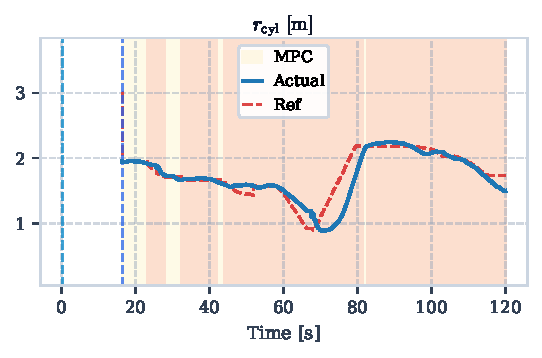
\includegraphics[width=\linewidth]{Immagini/Capitolo6/Experiments/CYL_POV_distance_r_cyl.pdf}
\end{subfigure}
\begin{subfigure}[b]{0.49\textwidth}
    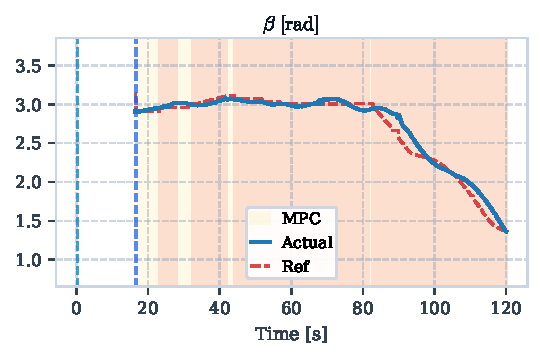
\includegraphics[width=\linewidth]{Immagini/Capitolo6/Experiments/CYL_POV_azimuth_beta.pdf}
\end{subfigure}
\begin{subfigure}[b]{0.49\textwidth}
    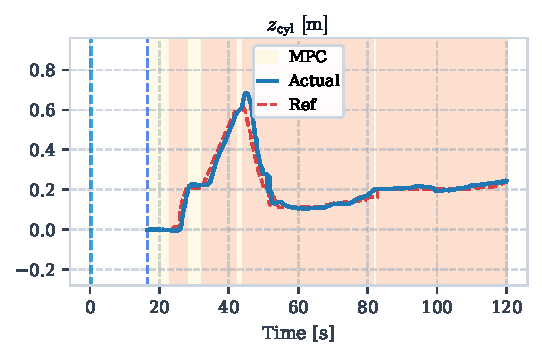
\includegraphics[width=\linewidth]{Immagini/Capitolo6/Experiments/CYL_POV_elevation_z.pdf}
\end{subfigure}
\begin{subfigure}[b]{0.49\textwidth}
    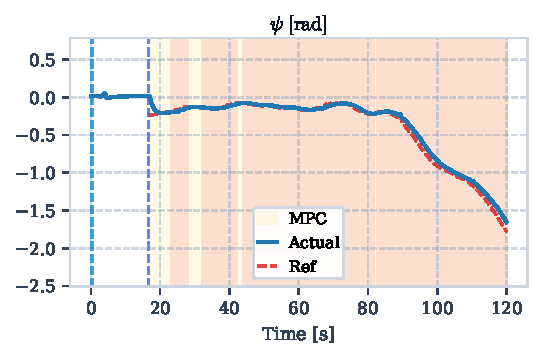
\includegraphics[width=\linewidth]{Immagini/Capitolo6/Experiments/YAW_yaw_actual_vs_desired.pdf}
\end{subfigure}
\caption{Cylindrical visual tracking variables along the real-world flight test}
\label{fig:hw_cyl_pov}
\end{figure}
The tracking performance in relative cylindrical coordinates is reported in Figure \ref{fig:hw_cyl_pov}. Despite the aerodynamic disturbances, the vehicle maintains the relative standoff distance with an RMS error of $0.18\text{ m}$, and controls elevation with high precision (RMS error of $3.1\text{ cm}$). The yaw orientation follows the relative azimuth smoothly, keeping the target centered in the camera frame with an RMS error of $3.07^\circ$.
\begin{figure}[h!]
\centering
\begin{subfigure}[b]{0.51\textwidth}
    
\includegraphics[width=\linewidth]{Immagini/Capitolo6/Experiments/phases_legend.pdf}
\end{subfigure}
\begin{subfigure}[b]{0.8\textwidth}
    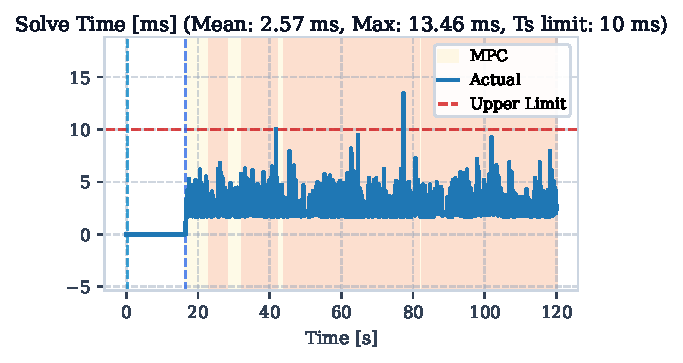
\includegraphics[width=\linewidth]{Immagini/Capitolo6/Experiments/SOLVE_TIME_solve_time.pdf}
\end{subfigure}
\caption{Onboard NMPC solving time on the LattePanda companion computer during experimental flight}
\label{fig:hw_solve_time}
\end{figure}
Figure \ref{fig:hw_solve_time} reports the execution time of the NMPC solver executed onboard the LattePanda computer throughout the flight. The solver demonstrates high computational efficiency: the mean execution time is $2.57\text{ ms}$, corresponding to an average CPU load of only $25.7\%$ within the $10\text{ ms}$ control step ($100\text{ Hz}$). The 99th percentile reaches $6.25\text{ ms}$, with solver overruns ($>10\text{ ms}$) limited to $0.08\%$ ($2$ cycles over $2649$), fully absorbed by the real-time iteration (SQP-RTI) scheme without inducing instability.

\begin{figure}[h!]
\centering
\begin{subfigure}[b]{0.51\textwidth}
    
\includegraphics[width=\linewidth]{Immagini/Capitolo6/Experiments/phases_legend.pdf}
\end{subfigure}
\begin{subfigure}[b]{0.8\textwidth}
    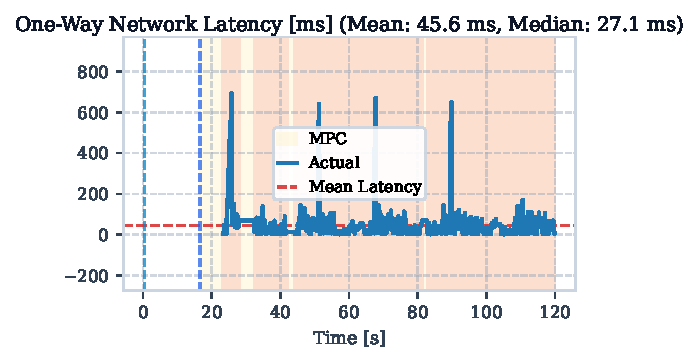
\includegraphics[width=\linewidth]{Immagini/Capitolo6/Experiments/HAPTIC_LATENCY_latency.pdf}
\end{subfigure}
\caption{One-way network communication latency of the bilateral haptic teleoperation channel during physical flight}
\label{fig:hw_haptic_latency}
\end{figure}
To assess the communication performance of the shared teleoperation loop over the local wireless link, Figure \ref{fig:hw_haptic_latency} reports the one-way network latency between the Ground Control Station (interfaced with the Novint Falcon) and the onboard companion computer. During active teleoperation phases (highlighted by the red shaded regions), the mean one-way latency is $45.56\text{ ms}$, with a median of $27.14\text{ ms}$ and a 95th percentile contained within $92.90\text{ ms}$. This latency profile satisfies standard haptic transparency requirements, allowing the human operator to receive responsive tactile feedback without inducing delay-driven instabilities.

To verify camera stability and the absence of high-frequency shakes during physical flight, Figure \ref{fig:hw_derivative_norms} reports the Euclidean norms of linear acceleration, angular acceleration, jerk, and snap recorded onboard.
\begin{figure}[h!]
\centering
\begin{subfigure}[b]{0.71\textwidth}
    
\includegraphics[width=\linewidth]{Immagini/Capitolo6/Experiments/phases_legend.pdf}
\end{subfigure}
\begin{subfigure}[b]{0.49\textwidth}
    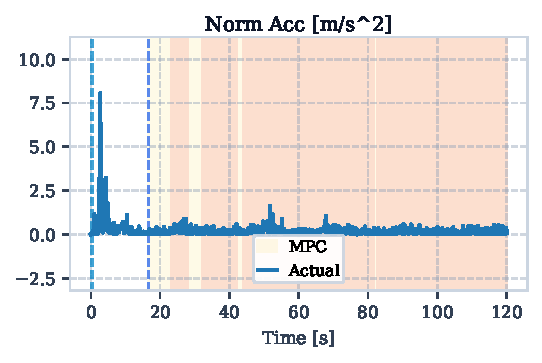
\includegraphics[width=\linewidth]{Immagini/Capitolo6/Experiments/DERIVATIVE_NORMS_norm_acc.pdf}
\end{subfigure}
\begin{subfigure}[b]{0.49\textwidth}
    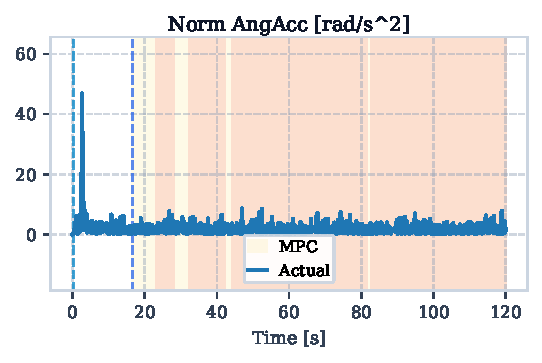
\includegraphics[width=\linewidth]{Immagini/Capitolo6/Experiments/DERIVATIVE_NORMS_norm_angacc.pdf}
\end{subfigure}
\begin{subfigure}[b]{0.49\textwidth}
    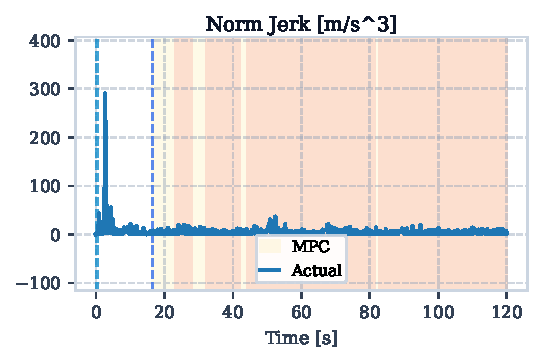
\includegraphics[width=\linewidth]{Immagini/Capitolo6/Experiments/DERIVATIVE_NORMS_norm_jerk.pdf}
\end{subfigure}
\begin{subfigure}[b]{0.49\textwidth}
    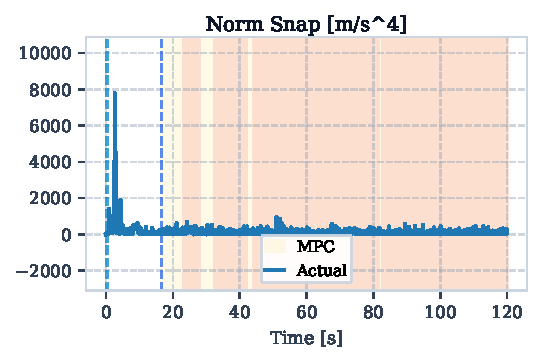
\includegraphics[width=\linewidth]{Immagini/Capitolo6/Experiments/DERIVATIVE_NORMS_norm_snap.pdf}
\end{subfigure}
\caption{Norms of higher-order dynamic derivatives penalised in the NMPC cost function during real-world flight}
\label{fig:hw_derivative_norms}
\end{figure}
As highlighted by the plots, the higher derivative norms remain strictly bounded throughout the test. Even under aerodynamical downwash and target speed changes, the high-frequency jerk and snap components are strongly penalized by the NMPC cost function, preventing jerky camera motions and potential motion sickness for the human operator.

\begin{figure}[h!]
\centering
\begin{subfigure}[b]{0.71\textwidth}
    
\includegraphics[width=\linewidth]{Immagini/Capitolo6/Experiments/phases_legend.pdf}
\end{subfigure}
\begin{subfigure}[b]{0.32\textwidth}
    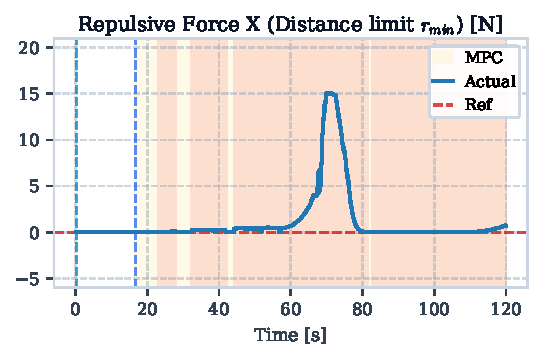
\includegraphics[width=\linewidth]{Immagini/Capitolo6/Experiments/REPULSIVE_FORCES_repulsive_force_x.pdf}
\end{subfigure}
\begin{subfigure}[b]{0.32\textwidth}
    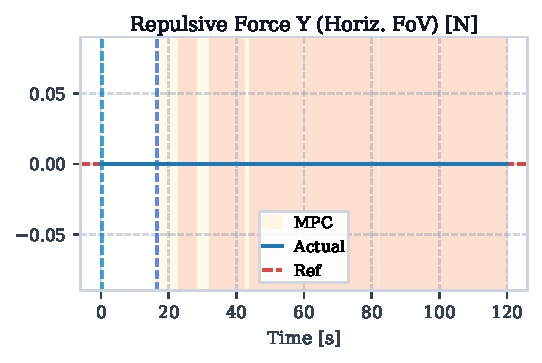
\includegraphics[width=\linewidth]{Immagini/Capitolo6/Experiments/REPULSIVE_FORCES_repulsive_force_y.pdf}
\end{subfigure}
\begin{subfigure}[b]{0.32\textwidth}
    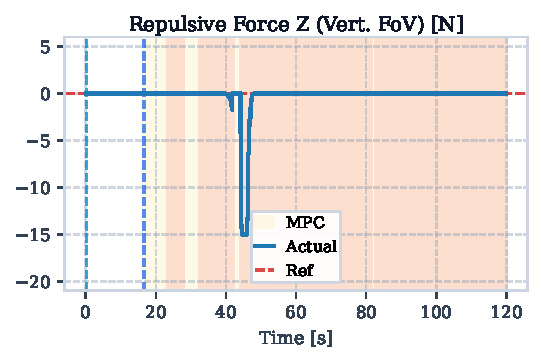
\includegraphics[width=\linewidth]{Immagini/Capitolo6/Experiments/REPULSIVE_FORCES_repulsive_force_z.pdf}
\end{subfigure}
\caption{Artificial potential field repulsive forces transmitted to the Novint Falcon haptic joystick during real-world flight}
\label{fig:hw_haptic_rep}
\end{figure}

\begin{figure}[h!]
\centering
\begin{subfigure}[b]{0.71\textwidth}
    
\includegraphics[width=\linewidth]{Immagini/Capitolo6/Experiments/phases_legend.pdf}
\end{subfigure}
\begin{subfigure}[b]{0.32\textwidth}
    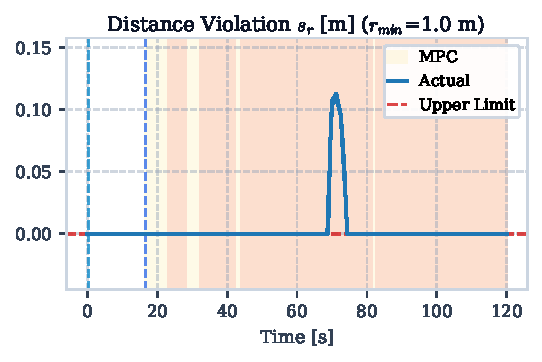
\includegraphics[width=\linewidth]{Immagini/Capitolo6/Experiments/APF_distance_violation_s_r.pdf}
\end{subfigure}
\begin{subfigure}[b]{0.32\textwidth}
    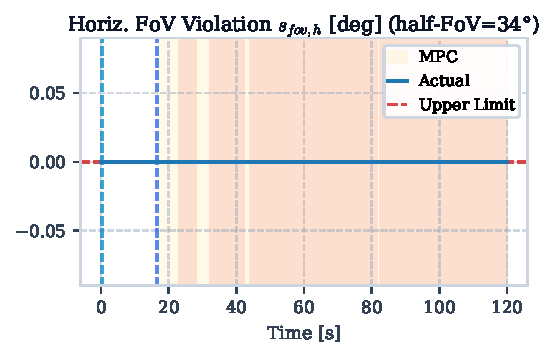
\includegraphics[width=\linewidth]{Immagini/Capitolo6/Experiments/APF_horiz_fov_violation_s__fov_h.pdf}
\end{subfigure}
\begin{subfigure}[b]{0.32\textwidth}
    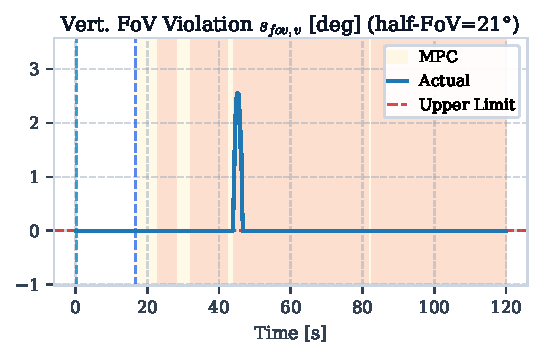
\includegraphics[width=\linewidth]{Immagini/Capitolo6/Experiments/APF_vert_fov_violation_s__fov_v.pdf}
\end{subfigure}
\caption{Safety distance and camera Field of View constraint violations during experimental flight}
\label{fig:hw_apf_violations}
\end{figure}

Figures \ref{fig:hw_haptic_rep} and \ref{fig:hw_apf_violations} illustrate the bilateral interaction between the human operator and the aerial platform through the Novint Falcon haptic interface. In our shared control formulation, the artificial potential field acts as an anticipatory safety barrier: when human teleoperation commands the vehicle towards an unfeasible configuration, exponential repulsive forces push the control handle back.
\\Specifically, during radial teleoperation around $t \approx 70\text{ s}$, the pilot pushes the joystick forward to inspect the target at close range. As the inter-drones distance approaches the safety boundary $r_{\min} = 1.0\text{ m}$ (with a transient encroachment peaking at $s_r = 0.11\text{ m}$), the repulsive force $F_x^{\text{rep}}$ rises steeply and reaches the physical saturation threshold of $15.0\text{ N}$. The strong tactile resistance informs the operator of the impending collision hazard, leading them to ease the forward pressure. As a result, the distance smoothly recovers beyond $1.5\text{ m}$, and $s_r$ promptly returns to zero.
\\A similar protective behavior occurs along the vertical direction around $t \approx 45\text{ s}$. When the operator commands an upward climb, bringing the target close to the upper limit of the vertical camera Field of View ($\text{FOV}_v = 42^\circ$, corresponding to a semi-aperture of $21^\circ$), the target slightly exceeds the viewing boundary ($s_{fov,v} = 2.56^\circ$). In response, the APF exerts a peak downward force $F_z^{\text{rep}} = -15.0\text{ N}$, saturated to $10 \text{N}$, on the joystick, prompting the human operator to lower the setpoint and immediately re-centering the target within the camera frame ($s_{fov,v} \to 0$).
\\Along the horizontal direction, because the autonomous yaw tracking loop maintains the optical axis tightly aligned with the target ($|\psi_{\text{err}}| \le 16.5^\circ$, well within the horizontal semi-aperture of $34.5^\circ$), the horizontal violation remains zero ($s_{fov,h} = 0^\circ$), resulting in $F_y^{\text{rep}} = 0\text{ N}$ throughout the flight, since it can be violated only with delays in azimuth $\beta$ tracking.
\\A quantitative comparison between the SITL simulation and the real-world flight test is summarized in Table \ref{tab:sitl_vs_hw}.
\begin{table}[htbp]
\centering
\small
\caption{Quantitative comparison between SITL simulation and physical flight experiment. ($^*$Evaluated during targeted haptic teleoperation tests: $s_r^{\max} = \SI{0.401}{\meter}$, $s_{fov,v}^{\max} = \ang{1.41}$, and $\|F_{\text{rep}}\|_{\infty} = \SI{10.00}{\newton}$ in SITL).}
\label{tab:sitl_vs_hw}
\resizebox{\columnwidth}{!}{
\begin{tabular}{lcc}
\toprule
\textbf{Metric} & \textbf{SITL Simulation} & \textbf{Real Experiment} \\
\midrule
Nominal Control Frequency ($1/T_s$) & \SI{100}{\hertz} & \SI{100}{\hertz} \\
Mean Solver Solve Time & \SI{0.91}{\milli\second} & \SI{2.57}{\milli\second} \\
Mean Solver CPU Load & \SI{9.1}{\percent} & \SI{25.7}{\percent} \\
99th Percentile Solve Time & \SI{1.37}{\milli\second} & \SI{6.25}{\milli\second} \\
Solver Overruns ($> \SI{10}{\milli\second}$) & \SI{0.00}{\percent} & \SI{0.08}{\percent} \\
\midrule
Radial Distance RMS Error ($r$) & \SI{0.107}{\meter} & \SI{0.183}{\meter} \\
Elevation RMS Error ($z_{rel}$) & \SI{0.073}{\meter} & \SI{0.031}{\meter} \\
Yaw RMS Error ($\psi$) & \ang{4.92} & \ang{3.07} \\
\midrule
Linear Velocity ($\|v\|$) RMS / Max & \SI{0.202}{\meter\per\second} / \SI{0.744}{\meter\per\second} & \SI{0.080}{\meter\per\second} / \SI{0.203}{\meter\per\second} \\
Angular Velocity ($\|\omega\|$) RMS / Max & \SI{0.046}{\radian\per\second} / \SI{0.282}{\radian\per\second} & \SI{0.081}{\radian\per\second} / \SI{0.257}{\radian\per\second} \\
Linear Acceleration ($\|a\|$) RMS / Max & \SI{0.166}{\meter\per\second\squared} / \SI{3.605}{\meter\per\second\squared} & \SI{0.193}{\meter\per\second\squared} / \SI{1.619}{\meter\per\second\squared} \\
\midrule
Max Distance Violation ($s_r$) & \SI{0.000}{\meter}$^*$ & \SI{0.113}{\meter} \\
Max Vert. FoV Violation ($s_{fov,v}$) & \ang{0.00}$^*$ & \ang{2.56} \\
Max Peak Repulsive Force ($\|F_{\text{rep}}\|_{\infty}$) & \SI{0.00}{\newton}$^*$ & \SI{15.00}{\newton} \\
Mean Haptic Latency & \SI{0.53}{\milli\second} & \SI{45.56}{\milli\second} \\
\bottomrule
\end{tabular}
}
\end{table}
As reported, the Observer UAV executes smooth tracking motions without aggressive velocity or acceleration demands. The linear velocity maintains an RMS of $0.08\text{ m/s}$ ($0.20\text{ m/s}$ max), and linear acceleration presents an RMS of $0.19\text{ m/s}^2$ ($1.62\text{ m/s}^2$ peak), confirming high mechanical stability and minimal vibration for the visual payload.
\\These experimental findings validate the full integration of autonomous optimal visual tracking with bilateral haptic shared control on physical embedded hardware. The artificial potential field reliably transfers perceptual safety cues to the pilot, preventing unsafe actions without restricting maneuverability during cooperative aerial operations.



    \chapter{Experimental Results}
    \section{Real-World Experimental Assessment}
To validate the proposed shared-control and tracking framework on real robotic hardware, flight tests were carried out exclusively on the Observer UAV.
As shown in Figure~\ref{fig:hw_observer_arena}, the experiments were conducted inside a dedicated indoor flight arena equipped with an OptiTrack motion capture system. The optical tracking infrastructure provides millimeter-accurate 6-DoF pose feedback for all vehicles at high rate, broadcasted over the local network. 
The physical Observer UAV, named \texttt{Pocho}, is a custom octocopter platform designed for high payload capacity and stability. It runs the full high-level NMPC pipeline directly onboard a LattePanda 3 Delta companion computer at $100\text{ Hz}$, interfaced with a Pixhawk 4 autopilot running the PX4 firmware via Micro-XRCE-DDS over a high-speed serial link. A second, manually piloted quadrotor acts as the dynamic physical target. 
The Ground Control Station (GCS) hosts the mission supervisor and the Novint Falcon haptic driver, exchanging setpoints, telemetries, and force commands with the onboard computer over a wireless Wi-Fi connection.
\begin{figure}[htbp]
    \centering
    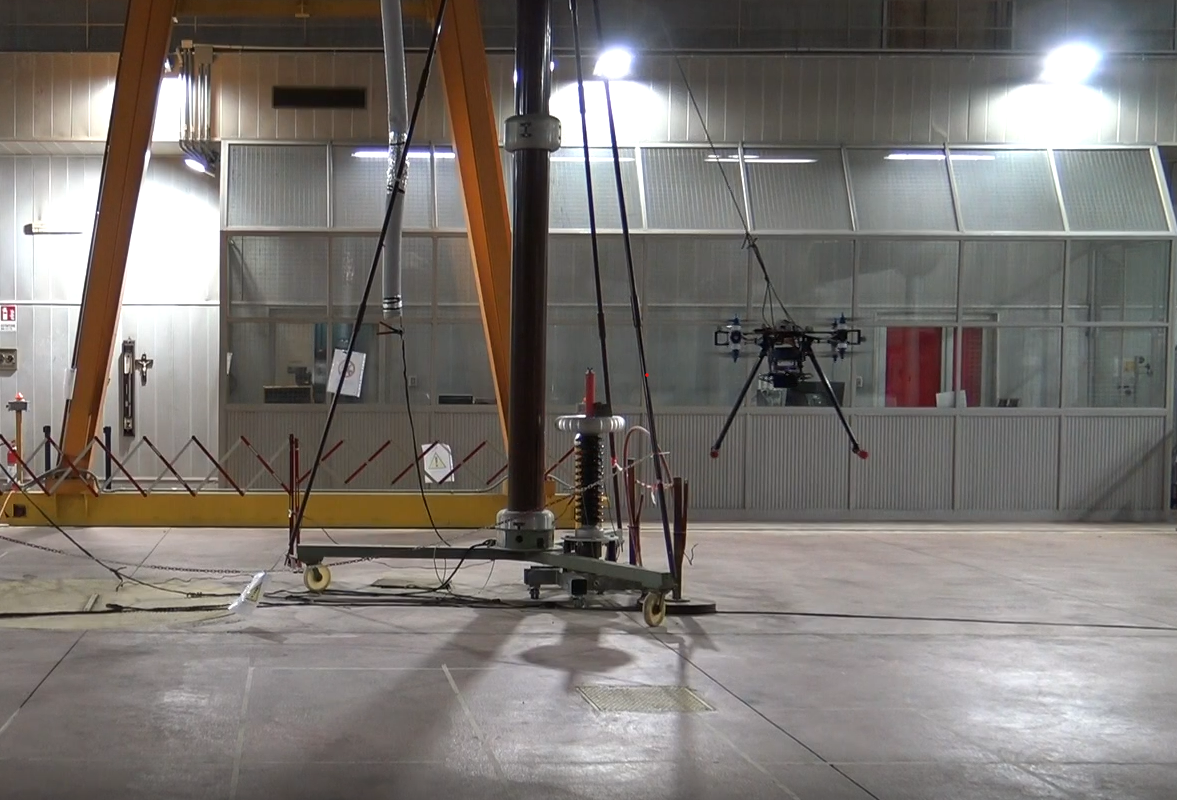
\includegraphics[width=0.75\linewidth]{Immagini/Capitolo7/Experiments/POCHO_flying_arena.png}
    \caption{Snapshot of the physical Observer Drone, \texttt{Pocho}, flying inside the OptiTrack arena during the experimental evaluation.}
    \label{fig:hw_observer_arena}
\end{figure}
The hardware test was intentionally focused on the Observer drone to assess its embedded tracking capabilities, real-time solver execution, and bilateral teleoperation under real aerodynamics, actuator dynamics, and sensor noise. To reduce the computational burden on the onboard companion computer, in these physical experiments jerk and snap penalty terms were omitted from the NMPC cost function. 
Two flight tests were conducted:
\begin{enumerate}
    \item \textbf{Bilateral Haptic Shared Teleoperation Flight:} where the operator actively assigns cylindrical setpoints using the Novint Falcon haptic device, testing online reference tracking, tactile perception, and the APF repulsive forces under human-in-the-loop control.
    \item \textbf{Partial Cooperative Mission Flight:} where the mission FSM commands sequential visual setpoints ($r, \beta, z_{rel}$) across the mission phases while the Observer tracks the moving target, evaluating autonomous viewpoint adaptation and phase progression without executing physical contact with the environment.
\end{enumerate}

\subsection{Bilateral Haptic Shared Teleoperation Flight}
In this first test, the operator interacts with the Novint Falcon haptic device to command time-varying cylindrical setpoints ($r, \beta, z_{rel}$) while the Observer UAV tracks the target quadrotor in real time.

\begin{figure}[htbp]
\centering
\begin{subfigure}[b]{0.71\textwidth}
    
\includegraphics[width=\linewidth]{Immagini/Capitolo7/Experiments/Haptic/phases_legend.pdf}
\end{subfigure}
\begin{subfigure}[b]{0.49\textwidth}
    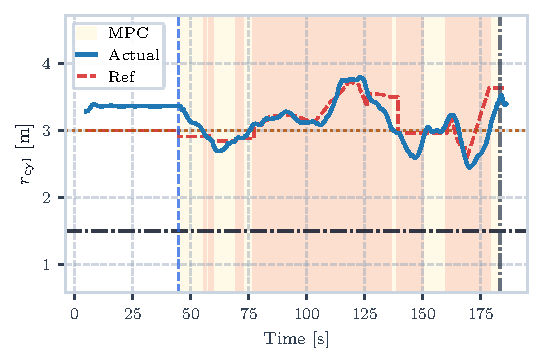
\includegraphics[width=\linewidth]{Immagini/Capitolo7/Experiments/Haptic/CYL_POV_distance_r_cyl.pdf}
\end{subfigure}
\begin{subfigure}[b]{0.49\textwidth}
    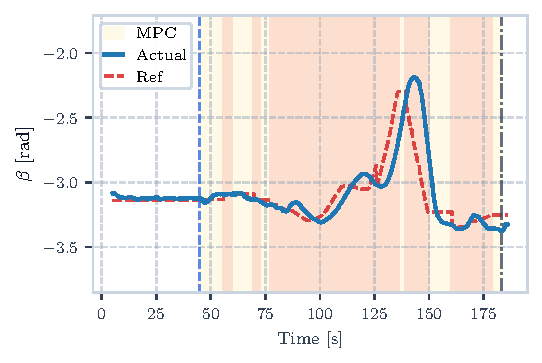
\includegraphics[width=\linewidth]{Immagini/Capitolo7/Experiments/Haptic/CYL_POV_azimuth_beta.pdf}
\end{subfigure}
\begin{subfigure}[b]{0.49\textwidth}
    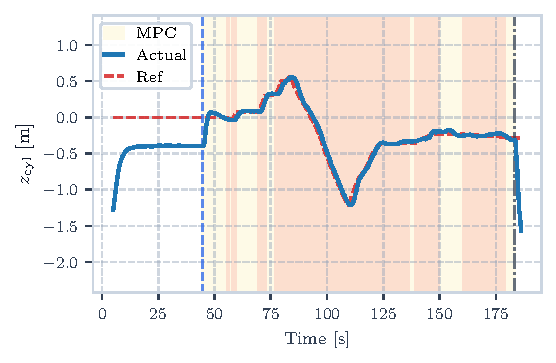
\includegraphics[width=\linewidth]{Immagini/Capitolo7/Experiments/Haptic/CYL_POV_elevation_z.pdf}
\end{subfigure}
\begin{subfigure}[b]{0.49\textwidth}
    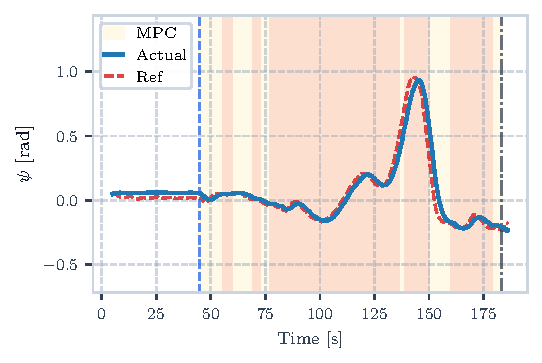
\includegraphics[width=\linewidth]{Immagini/Capitolo7/Experiments/Haptic/YAW_yaw_actual_vs_desired.pdf}
\end{subfigure}
\caption{Cylindrical visual tracking variables during the real-world bilateral haptic teleoperation flight.}
\label{fig:hw_haptic_cyl_pov}
\end{figure}
\justify
Figure~\ref{fig:hw_haptic_cyl_pov} illustrates the tracking performance of the cylindrical coordinates and camera yaw orientation throughout the flight. The colored background bands indicate the active mission phases, during which the human operator continuously commands viewpoint adjustments:
\begin{itemize}
    \item The radial standoff distance $r$ starts from the initial hovering distance ($1.5\text{ m}$) and is actively modified by the operator via the joystick. Despite target velocity variations and real-world disturbances and uncertainties, the observer closely follows the reference, yielding an RMS tracking error of $0.223\text{ m}$ with a maximum deviation of $0.684\text{ m}$.
    \item The azimuth angle $\beta$ shows that the operator successfully commands viewpoint rotations around the target vehicle across different angular sectors. The NMPC navigates the vehicle smoothly along the cylindrical arc, achieving an RMS tracking error of $10.45^\circ$, with a maximum transient peak of $38.94^\circ$ occurring during rapid manual setpoint variations.
    \item The relative elevation $z_{rel}$ demonstrates accurate vertical regulation. The RMS vertical tracking error is limited to $0.062\text{ m}$ ($6.19\text{ cm}$), with a maximum error of $0.398\text{ m}$.
    \item The yaw angle $\psi$ tracks the desired line-of-sight angle computed to point the camera optical axis towards the target drone. The actual yaw closely matches the desired orientation with an RMS error of $4.08^\circ$ (maximum $15.24^\circ$), confirming that the target remains framed in the camera view throughout the teleoperation maneuvers.
\end{itemize}
As shown by the tracking error profiles in Figure~\ref{fig:hw_haptic_cyl_err}, the error norms remain bounded around zero during steady hovering and smooth tracking phases. Error peaks appear only in correspondence with rapid manual setpoint variations or aggressive target maneuvers, after which the NMPC quickly restores visual regulation. In particular, the vertical tracking error $|e_z|$ stays within a few centimeters for almost the entire flight, while the radial distance error $|e_r|$ exhibits higher deviations but without drifting (maximum $60$ cm in correspondence of cumulating references, due to haptic latency), confirming viewpoint maintenance under real aerodynamic disturbances.

\begin{figure}[htbp]
\centering
\begin{subfigure}[b]{0.71\textwidth}
    
\includegraphics[width=\linewidth]{Immagini/Capitolo7/Experiments/Haptic/phases_legend.pdf}
\end{subfigure}
\begin{subfigure}[b]{0.49\textwidth}
    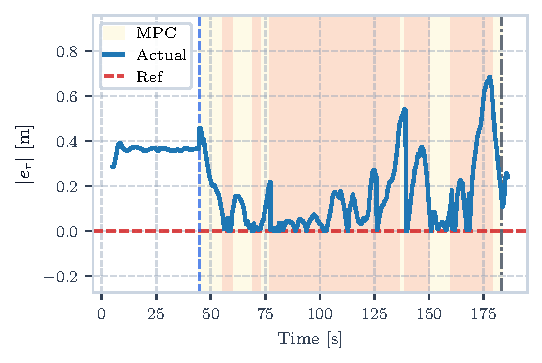
\includegraphics[width=\linewidth]{Immagini/Capitolo7/Experiments/Haptic/CYL_POV_ERR_distance_error_r_cyl_err.pdf}
\end{subfigure}
\begin{subfigure}[b]{0.49\textwidth}
    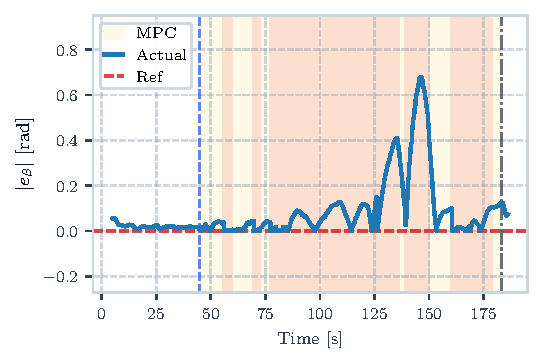
\includegraphics[width=\linewidth]{Immagini/Capitolo7/Experiments/Haptic/CYL_POV_ERR_azimuth_error_beta_err.pdf}
\end{subfigure}
\begin{subfigure}[b]{0.49\textwidth}
    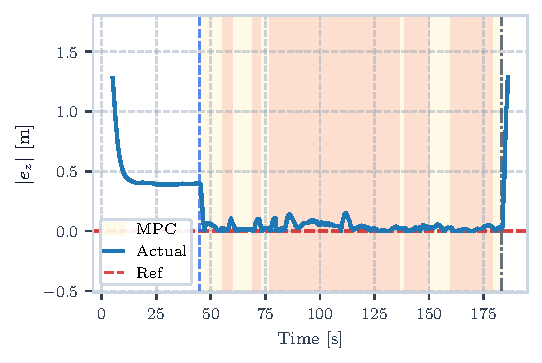
\includegraphics[width=\linewidth]{Immagini/Capitolo7/Experiments/Haptic/CYL_POV_ERR_elevation_error_z_err.pdf}
\end{subfigure}
\begin{subfigure}[b]{0.49\textwidth}
    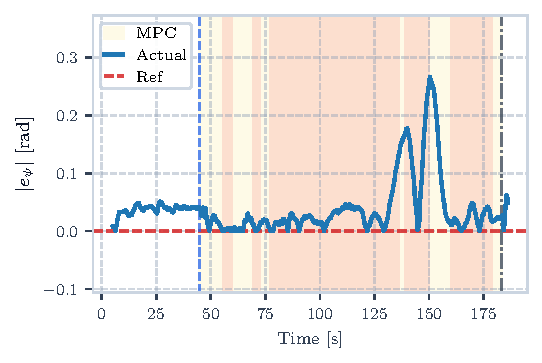
\includegraphics[width=\linewidth]{Immagini/Capitolo7/Experiments/Haptic/CYL_POV_ERR_yaw_error_yaw_err.pdf}
\end{subfigure}
\caption{Tracking error norms on cylindrical coordinates and yaw orientation during the haptic teleoperation flight.}
\label{fig:hw_haptic_cyl_err}
\end{figure}


\begin{figure}[h!]
\centering
\begin{subfigure}[b]{0.51\textwidth}
    
\includegraphics[width=\linewidth]{Immagini/Capitolo7/Experiments/Haptic/phases_legend.pdf}
\end{subfigure}
\begin{subfigure}[b]{0.8\textwidth}
    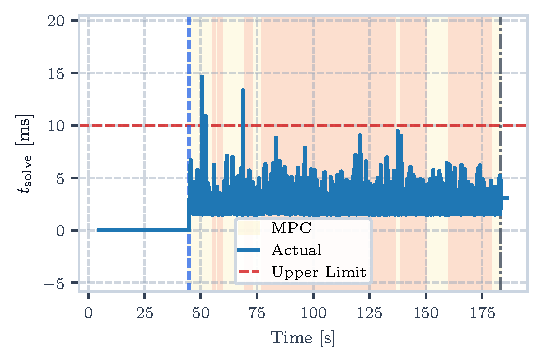
\includegraphics[width=\linewidth]{Immagini/Capitolo7/Experiments/Haptic/SOLVE_TIME_solve_time.pdf}
\end{subfigure}
\caption{Onboard NMPC solving time on the LattePanda companion computer during the haptic teleoperation flight.}
\label{fig:hw_haptic_solve_time}
\end{figure}
\justify
Figure~\ref{fig:hw_haptic_solve_time} reports the execution time of the NMPC solver running onboard the LattePanda companion computer. The mean solve time is $2.29\text{ ms}$, which corresponds to a CPU load of only $22.9\%$ of the available $10\text{ ms}$ sampling period at $100\text{ Hz}$. The 99th percentile of the execution time is $5.88\text{ ms}$, leaving substantial computational headroom for background ROS 2 communications and sensor drivers. Over the entire flight test comprising 3415 consecutive control cycles, only 3 deadline overruns ($>10\text{ ms}$) were detected ($0.09\%$). These isolated delays were quickly absorbed in subsequent cycles without causing any loss of control authority.

\begin{figure}[htbp]
\centering
\begin{subfigure}[b]{0.51\textwidth}
    
\includegraphics[width=\linewidth]{Immagini/Capitolo7/Experiments/Haptic/phases_legend.pdf}
\end{subfigure}
\begin{subfigure}[b]{0.8\textwidth}
    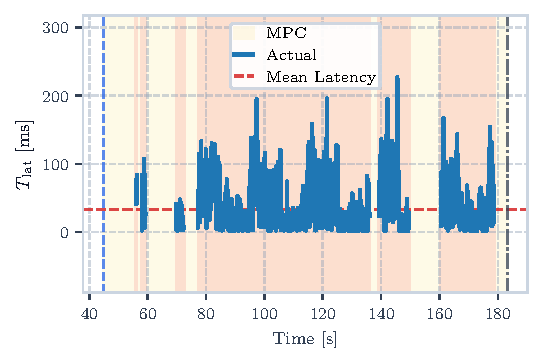
\includegraphics[width=\linewidth]{Immagini/Capitolo7/Experiments/Haptic/HAPTIC_LATENCY_latency.pdf}
\end{subfigure}
\caption{One-way network communication latency of the bilateral haptic teleoperation channel during physical flight.}
\label{fig:hw_haptic_latency}
\end{figure}
\justify
Figure~\ref{fig:hw_haptic_latency} shows the one-way network latency between the Ground Control Station and the onboard companion computer. The communication channel relies on a standard Wi-Fi link transmitting operator setpoints and receiving drone telemetry. The average latency is $32.77\text{ ms}$, with a 95th percentile of $107.04\text{ ms}$. This latency profile proved sufficiently bounded to preserve stability of the bilateral shared-control loop, allowing the operator to perceive force feedback with minimal tactile delay.
\begin{figure}[htbp]
\centering
\begin{subfigure}[b]{0.71\textwidth}
    
\includegraphics[width=\linewidth]{Immagini/Capitolo7/Experiments/Haptic/phases_legend.pdf}
\end{subfigure}
\begin{subfigure}[b]{0.49\textwidth}
    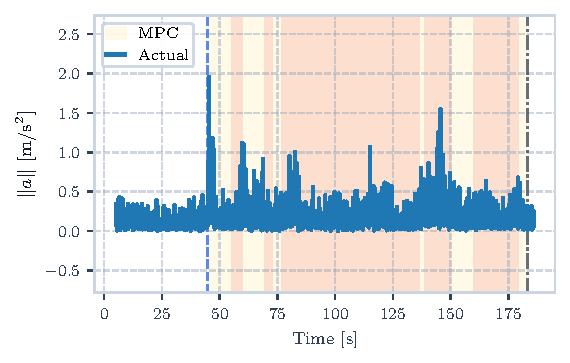
\includegraphics[width=\linewidth]{Immagini/Capitolo7/Experiments/Haptic/DERIVATIVE_NORMS_norm_acc.pdf}
\end{subfigure}
\begin{subfigure}[b]{0.49\textwidth}
    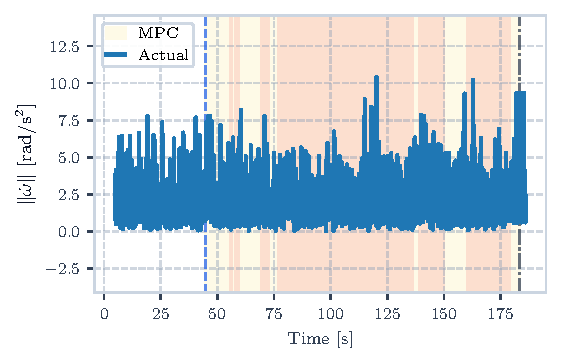
\includegraphics[width=\linewidth]{Immagini/Capitolo7/Experiments/Haptic/DERIVATIVE_NORMS_norm_angacc.pdf}
\end{subfigure}
\begin{subfigure}[b]{0.49\textwidth}
    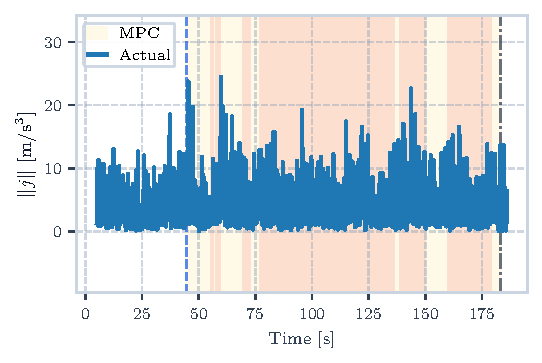
\includegraphics[width=\linewidth]{Immagini/Capitolo7/Experiments/Haptic/DERIVATIVE_NORMS_norm_jerk.pdf}
\end{subfigure}
\begin{subfigure}[b]{0.49\textwidth}
    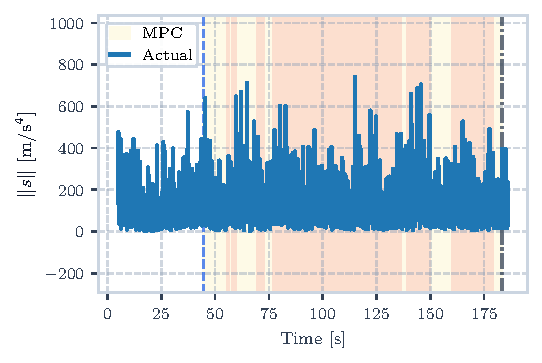
\includegraphics[width=\linewidth]{Immagini/Capitolo7/Experiments/Haptic/DERIVATIVE_NORMS_norm_snap.pdf}
\end{subfigure}
\caption{Norms of higher-order dynamic derivatives recorded during the haptic flight test.}
\label{fig:hw_haptic_derivative_norms}
\end{figure}
\justify
About higher-order time derivatives, figure~\ref{fig:hw_haptic_derivative_norms} presents the norms of linear acceleration $\|a\|$, angular acceleration $\|\dot{\omega}\|$, jerk $\|j\|$, and snap $\|s\|$ recorded during the teleoperation flight. It is worth noting that, in order to keep the solver lightweight on the embedded companion computer, jerk and snap penalty terms were not included in the NMPC cost function during hardware flights. Nevertheless, the physical response remained smooth across all axes: linear acceleration maintained an RMS norm of $0.241\text{ m/s}^2$ (with a peak of $1.95\text{ m/s}^2$ during aggressive maneuvers), and angular velocity had an RMS of $0.099\text{ rad/s}$. The jerk and snap norms show no high-frequency oscillations or chattering, demonstrating that the underlying rigid-body dynamics model and state constraints in the NMPC formulation are sufficient to ensure clean flight behavior.
\\This smooth behavior is also directly reflected in the control wrench, as illustrated in Figure~\ref{fig:hw_haptic_control_wrench}. The vertical thrust $F_z$ stays centered around the nominal hover value ($\approx 37.2\text{ N}$), adapting smoothly to track vertical maneuvers without actuator saturation. The commanded torques remain small and chattering-free; notably, the pitch torque $\tau_y$ shows a consistent steady-state offset around $-0.17\text{ N}\cdot\text{m}$, compensating for the unmodeled forward center-of-mass shift caused by the camera and mounting hardware. The controller easily handles this structural asymmetry, keeping attitude and tracking stable without requiring ad-hoc integrator states.

\begin{figure}[htbp]
\centering
\begin{subfigure}[b]{0.71\textwidth}
    
\includegraphics[width=\linewidth]{Immagini/Capitolo7/Experiments/Haptic/phases_legend.pdf}
\end{subfigure}
\begin{subfigure}[b]{0.49\textwidth}
    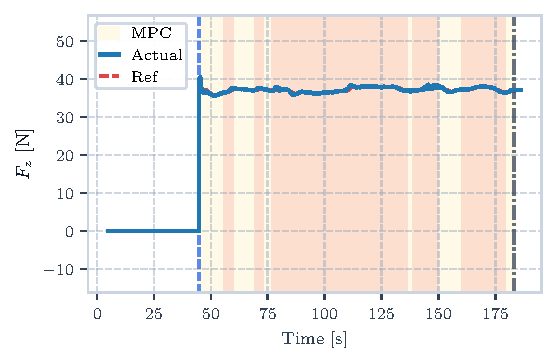
\includegraphics[width=\linewidth]{Immagini/Capitolo7/Experiments/Haptic/CONTROL_WRENCH_force_z.pdf}
\end{subfigure}
\begin{subfigure}[b]{0.49\textwidth}
    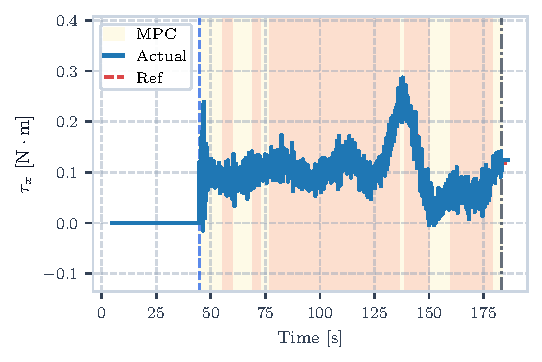
\includegraphics[width=\linewidth]{Immagini/Capitolo7/Experiments/Haptic/CONTROL_WRENCH_torque_x.pdf}
\end{subfigure}
\begin{subfigure}[b]{0.49\textwidth}
    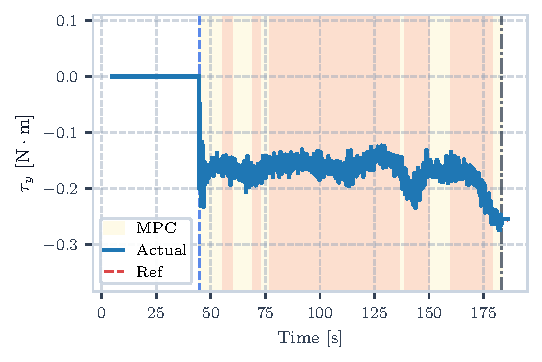
\includegraphics[width=\linewidth]{Immagini/Capitolo7/Experiments/Haptic/CONTROL_WRENCH_torque_y.pdf}
\end{subfigure}
\begin{subfigure}[b]{0.49\textwidth}
    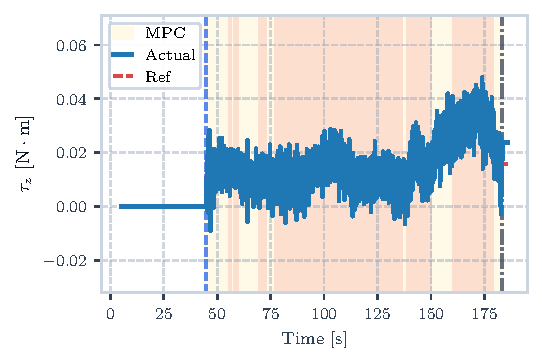
\includegraphics[width=\linewidth]{Immagini/Capitolo7/Experiments/Haptic/CONTROL_WRENCH_torque_z.pdf}
\end{subfigure}
\caption{Control wrench components ($F_z, \tau_x, \tau_y, \tau_z$) commanded by the NMPC during the haptic flight test.}
\label{fig:hw_haptic_control_wrench}
\end{figure}

\begin{figure}[htbp]
\centering
\begin{subfigure}[b]{0.71\textwidth}
    
\includegraphics[width=\linewidth]{Immagini/Capitolo7/Experiments/Haptic/phases_legend.pdf}
\end{subfigure}
\begin{subfigure}[b]{0.32\textwidth}
    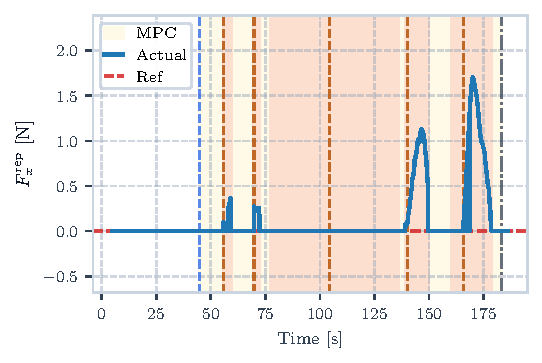
\includegraphics[width=\linewidth]{Immagini/Capitolo7/Experiments/Haptic/REPULSIVE_FORCES_repulsive_force_x.pdf}
\end{subfigure}
\begin{subfigure}[b]{0.32\textwidth}
    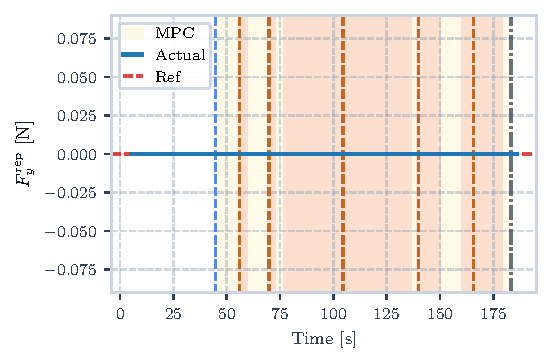
\includegraphics[width=\linewidth]{Immagini/Capitolo7/Experiments/Haptic/REPULSIVE_FORCES_repulsive_force_y.pdf}
\end{subfigure}
\begin{subfigure}[b]{0.32\textwidth}
    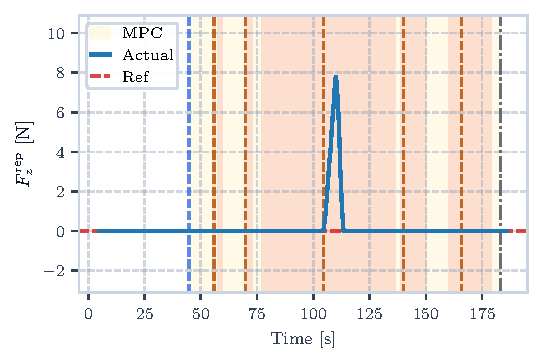
\includegraphics[width=\linewidth]{Immagini/Capitolo7/Experiments/Haptic/REPULSIVE_FORCES_repulsive_force_z.pdf}
\end{subfigure}
\caption{Artificial potential field repulsive forces transmitted to the Novint Falcon joystick during the haptic flight.}
\label{fig:hw_haptic_rep}
\end{figure}

\begin{figure}[htbp]
\centering
\begin{subfigure}[b]{0.71\textwidth}
    
\includegraphics[width=\linewidth]{Immagini/Capitolo7/Experiments/Haptic/phases_legend.pdf}
\end{subfigure}
\begin{subfigure}[b]{0.32\textwidth}
    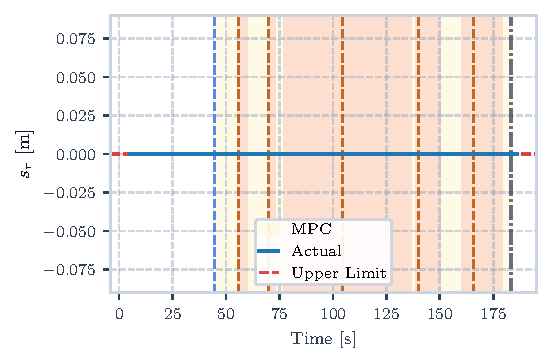
\includegraphics[width=\linewidth]{Immagini/Capitolo7/Experiments/Haptic/APF_distance_violation_s_r.pdf}
\end{subfigure}
\begin{subfigure}[b]{0.32\textwidth}
    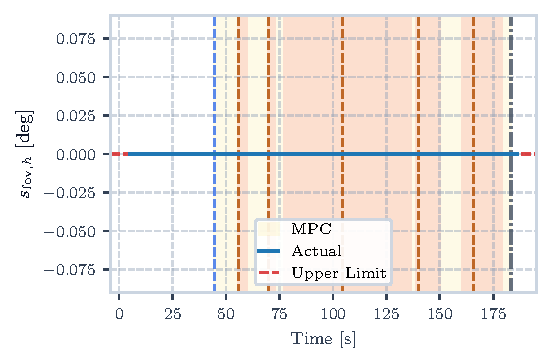
\includegraphics[width=\linewidth]{Immagini/Capitolo7/Experiments/Haptic/APF_horiz_fov_violation_s__fov_h.pdf}
\end{subfigure}
\begin{subfigure}[b]{0.32\textwidth}
    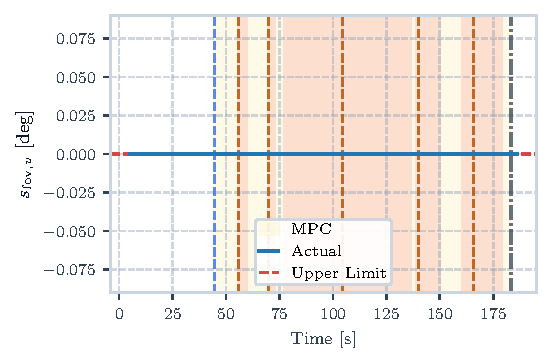
\includegraphics[width=\linewidth]{Immagini/Capitolo7/Experiments/Haptic/APF_vert_fov_violation_s__fov_v.pdf}
\end{subfigure}
\caption{Safety distance and camera Field of View constraint violations during the haptic flight.}
\label{fig:hw_haptic_apf_violations}
\end{figure}
\justify
Figures~\ref{fig:hw_haptic_rep} and \ref{fig:hw_haptic_apf_violations} illustrate the bilateral haptic interaction generated by the Artificial Potential Field (APF). Figure~\ref{fig:hw_haptic_rep} displays the three Cartesian components of the repulsive force ($F_x^{\text{rep}}, F_y^{\text{rep}}, F_z^{\text{rep}}$) sent to the Novint Falcon device, while Figure~\ref{fig:hw_haptic_apf_violations} shows the monitoring of the hard boundary slack variables ($s_r, s_{\text{fov},h}, s_{\text{fov},v}$).
It is worth remarking the relationship between these two figures: as formulated in Section 4.3, the repulsive field does not wait for a hard constraint violation to occur, but activates within an anticipatory buffer zone ($d < d_{\text{act}}$). For the radial distance, the activation threshold is $d_{\text{act}} = 1.5\text{ m}$, meaning tactile resistance begins as soon as $r < 3.0\text{ m}$. In this test, the pilot commanded the drone down to a minimum standoff distance of $2.5\text{ m}$, entering the outer margin of the repulsive zone and receiving a progressive force peaking at $F_x^{\text{rep}} = 1.71\text{ N}$ that discouraged closer approach. Similarly, when commanding vertical viewpoint variations, as the target entered the bottom $30\%$ of the camera frame, the APF rendered an upward repulsive force peaking at $F_z^{\text{rep}} = 7.78\text{ N}$. Guided by this prompt tactile feedback, the operator intuitively adjusted the joystick commands, preventing the vehicle from ever breaching the physical safety distance or losing target line-of-sight. As a result, the boundary violation slacks in Figure~\ref{fig:hw_haptic_apf_violations} remain strictly zero throughout the flight ($s_r = 0.00\text{ m}$, $s_{\text{fov},h} = 0.00^\circ$, $s_{\text{fov},v} = 0.00^\circ$).
\\A comprehensive quantitative summary of the performance metrics for this physical haptic teleoperation flight is reported in Table~\ref{tab:hw_haptic_metrics}.

\begin{table}[htbp]
\centering
\small
\caption{Performance metrics for the real-world bilateral haptic shared teleoperation flight test.}
\label{tab:hw_haptic_metrics}
\begin{tabular}{lc}
\toprule
\textbf{Metric} & \textbf{Value} \\
\midrule
Nominal Control Frequency ($1/T_s$) & \SI{100}{\hertz} \\
Mean Solver Solve Time & \SI{2.29}{\milli\second} (CPU Load: \SI{22.9}{\percent}) \\
99th Percentile Solve Time & \SI{5.88}{\milli\second} \\
Solver Overruns ($> \SI{10}{\milli\second}$) & \SI{0.09}{\percent} ($3 / 3415$) \\
\midrule
Radial Distance RMS / Max Error ($r$) & \SI{0.223}{\meter} / \SI{0.684}{\meter} \\
Azimuth Angle RMS / Max Error ($\beta$) & \ang{10.45} / \ang{38.94} \\
Elevation RMS / Max Error ($z_{rel}$) & \SI{0.062}{\meter} / \SI{0.398}{\meter} \\
Yaw Angle RMS / Max Error ($\psi$) & \ang{4.08} / \ang{15.24} \\
\midrule
Linear Velocity ($\|v\|$) RMS / Max & \SI{0.145}{\meter\per\second} / \SI{0.725}{\meter\per\second} \\
Angular Velocity ($\|\omega\|$) RMS / Max & \SI{0.099}{\radian\per\second} / \SI{0.577}{\radian\per\second} \\
Linear Acceleration ($\|a\|$) RMS / Max & \SI{0.241}{\meter\per\second\squared} / \SI{1.953}{\meter\per\second\squared} \\
\midrule
Max Distance Violation ($s_r$) & \SI{0.000}{\meter} \\
Max Horizontal FoV Violation ($s_{\text{fov},h}$) & \ang{0.00} \\
Max Vertical FoV Violation ($s_{\text{fov},v}$) & \ang{0.00} \\
Max Peak Repulsive Force ($\|F_{\text{rep}}\|_{\infty}$) & \SI{7.78}{\newton} \\
Mean One-Way Haptic Latency & \SI{32.77}{\milli\second} \\
\bottomrule
\end{tabular}
\end{table}

\subsection{Partial Mission Flight Test}
The second physical experiment evaluates the autonomous execution of a partial cooperative mission. In this test, the mission Finite State Machine orchestrates the sequential phases (Takeoff, Approach, Interaction, Detachment, Landing), updating the nominal cylindrical setpoints $(r, \beta, z_{rel})$ at each phase transition. The target quadrotor was flown manually inside the arena to provide an active, moving target, while the Observer UAV executed autonomous trajectory tracking and viewpoint reconfiguration without performing physical contact with the environment.

\begin{figure}[htbp]
\centering
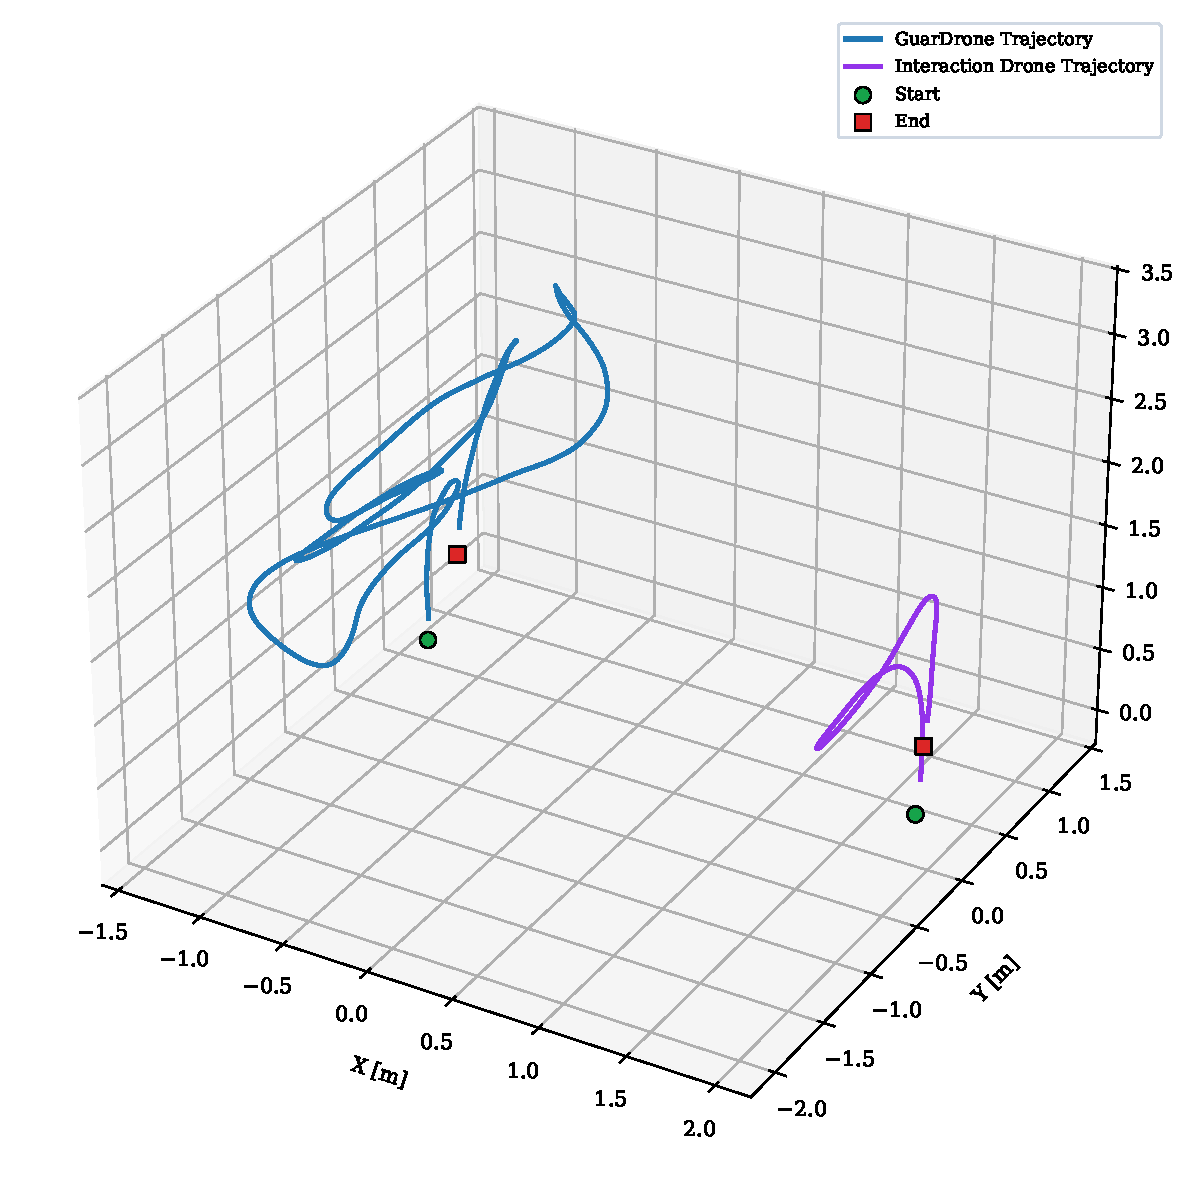
\includegraphics[width=0.55\linewidth]{Immagini/Capitolo7/Experiments/Mission/3D.pdf}
\caption{3D trajectories of the Observer and Target UAVs during the partial mission flight test.}
\label{fig:hw_mission_3d}
\end{figure}
\justify
Figure~\ref{fig:hw_mission_3d} shows the spatial trajectories of both vehicles reconstructed from OptiTrack telemetry. The Observer UAV continuously tracks the target across the three-dimensional volume, maintaining the commanded standoff distance and circling around it to achieve the perspective required by each operational phase.

\begin{figure}[htbp]
\centering
\begin{subfigure}[b]{0.71\textwidth}
    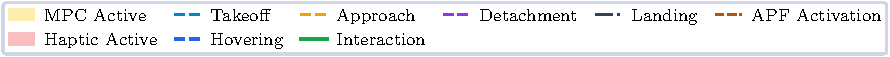
\includegraphics[width=\linewidth]{Immagini/Capitolo7/Experiments/Mission/phases_legend.pdf}
\end{subfigure}
\begin{subfigure}[b]{0.49\textwidth}
    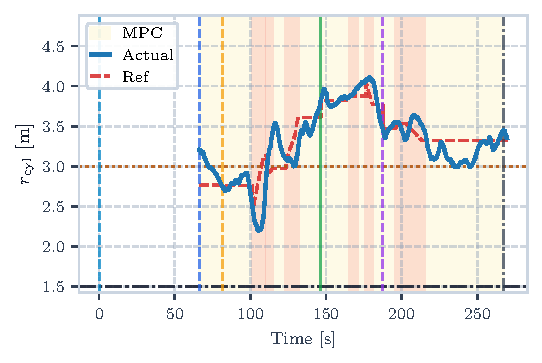
\includegraphics[width=\linewidth]{Immagini/Capitolo7/Experiments/Mission/CYL_POV_distance_r_cyl.pdf}
\end{subfigure}
\begin{subfigure}[b]{0.49\textwidth}
    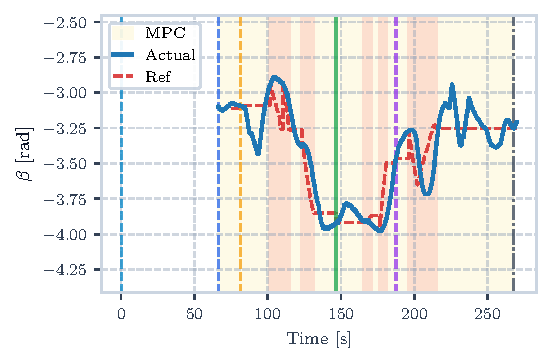
\includegraphics[width=\linewidth]{Immagini/Capitolo7/Experiments/Mission/CYL_POV_azimuth_beta.pdf}
\end{subfigure}
\begin{subfigure}[b]{0.49\textwidth}
    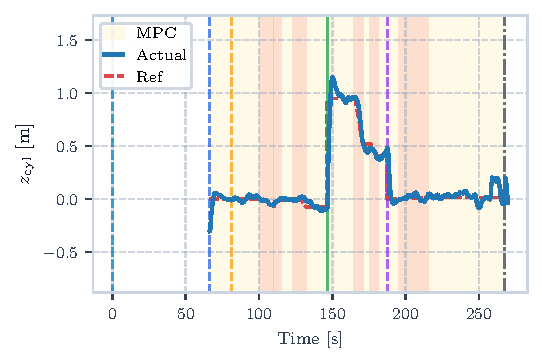
\includegraphics[width=\linewidth]{Immagini/Capitolo7/Experiments/Mission/CYL_POV_elevation_z.pdf}
\end{subfigure}
\begin{subfigure}[b]{0.49\textwidth}
    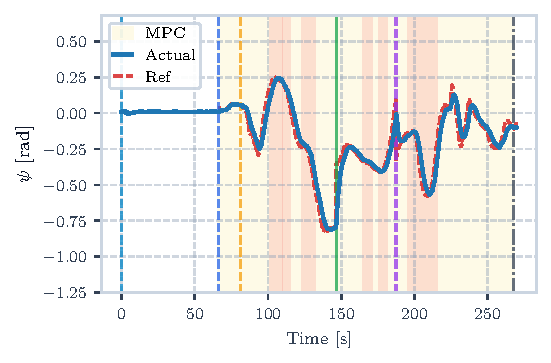
\includegraphics[width=\linewidth]{Immagini/Capitolo7/Experiments/Mission/YAW_yaw_actual_vs_desired.pdf}
\end{subfigure}
\caption{Cylindrical visual tracking variables during the real-world partial mission flight test.}
\label{fig:hw_mission_cyl_pov}
\end{figure}
\justify
Figure~\ref{fig:hw_mission_cyl_pov} details the tracking of the relative cylindrical coordinates across the mission phases:
\begin{itemize}
    \item The radial distance $r$ transitions from takeoff to the nominal standoff distance ($1.5\text{ m}$) and follows the phase references with an RMS error of $0.214\text{ m}$ (max $0.768\text{ m}$).
    \item The azimuth angle $\beta$ tracks the discrete step changes commanded by the supervisor between consecutive mission phases, demonstrating smooth convergence to the new perspective with an RMS error of $8.58^\circ$ (maximum transient deviation of $23.07^\circ$).
    \item The relative elevation $z_{rel}$ adapts to the nominal altitude offsets prescribed by the FSM, achieving an RMS tracking error of $0.082\text{ m}$ ($8.20\text{ cm}$) with a maximum error of $1.040\text{ m}$.
    \item The yaw orientation $\psi$ continuously aligns with the target heading reference, maintaining an RMS tracking error of $3.98^\circ$ (maximum $25.30^\circ$).
\end{itemize}
These results confirm that the NMPC tracker smoothly absorbs discrete phase step references, preserving trajectory continuity without inducing overshoot or flight instability.

The tracking errors on the cylindrical variables are shown in Figure~\ref{fig:hw_mission_cyl_err}. In this test, each phase transition commanded by the FSM introduces a discrete step in the reference (such as the viewpoint shift entering the Interaction phase). As it is visible from the plots, these steps produce temporary transient errors that the NMPC promptly rejects within a few seconds, driving the errors back to zero. Even under the continuous manual motion of the target vehicle, the radial distance error $|e_r|$ maintains an RMS of $0.214\text{ m}$ and the azimuth error $|e_\beta|$ stays at $8.58^\circ$, demonstrating effective viewpoint synchronization across all phases.

\begin{figure}[htbp]
\centering
\begin{subfigure}[b]{0.71\textwidth}
    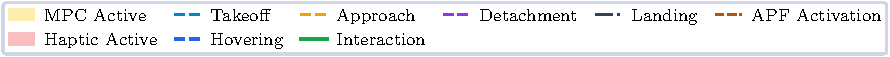
\includegraphics[width=\linewidth]{Immagini/Capitolo7/Experiments/Mission/phases_legend.pdf}
\end{subfigure}
\begin{subfigure}[b]{0.49\textwidth}
    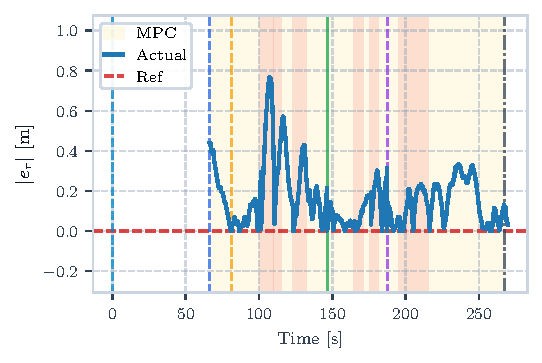
\includegraphics[width=\linewidth]{Immagini/Capitolo7/Experiments/Mission/CYL_POV_ERR_distance_error_r_cyl_err.pdf}
\end{subfigure}
\begin{subfigure}[b]{0.49\textwidth}
    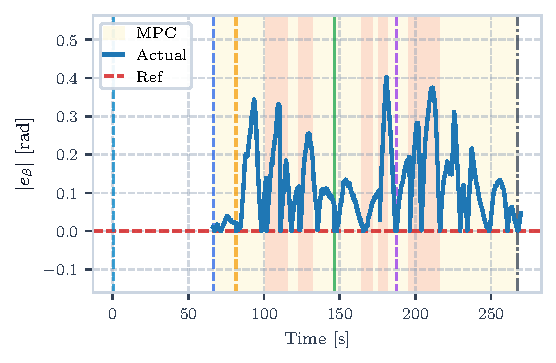
\includegraphics[width=\linewidth]{Immagini/Capitolo7/Experiments/Mission/CYL_POV_ERR_azimuth_error_beta_err.pdf}
\end{subfigure}
\begin{subfigure}[b]{0.49\textwidth}
    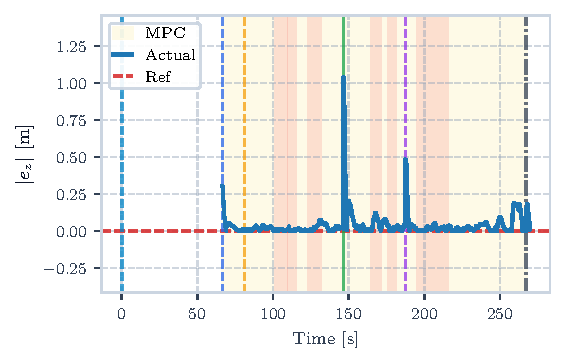
\includegraphics[width=\linewidth]{Immagini/Capitolo7/Experiments/Mission/CYL_POV_ERR_elevation_error_z_err.pdf}
\end{subfigure}
\begin{subfigure}[b]{0.49\textwidth}
    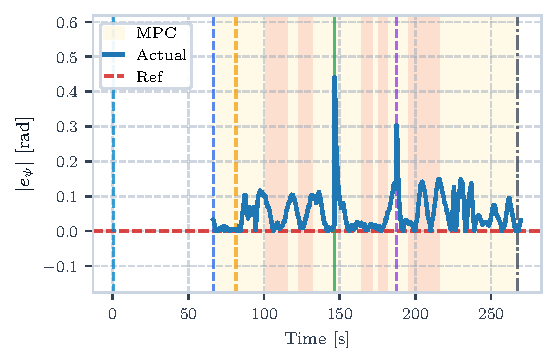
\includegraphics[width=\linewidth]{Immagini/Capitolo7/Experiments/Mission/CYL_POV_ERR_yaw_error_yaw_err.pdf}
\end{subfigure}
\caption{Tracking error norms on cylindrical coordinates and yaw orientation during the mission flight test.}
\label{fig:hw_mission_cyl_err}
\end{figure}


\begin{figure}[htbp]
\centering
\begin{subfigure}[b]{0.49\textwidth}
    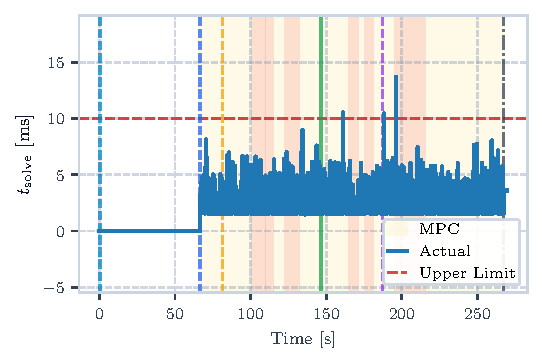
\includegraphics[width=\linewidth]{Immagini/Capitolo7/Experiments/Mission/SOLVE_TIME_solve_time.pdf}
    \caption{Onboard NMPC solving time}
    \label{fig:hw_mission_solve_time}
\end{subfigure}
\hfill
\begin{subfigure}[b]{0.49\textwidth}
    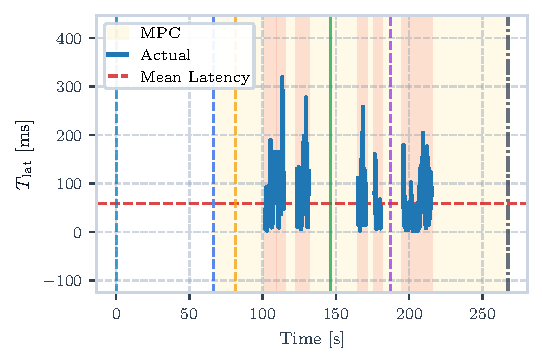
\includegraphics[width=\linewidth]{Immagini/Capitolo7/Experiments/Mission/HAPTIC_LATENCY_latency.pdf}
    \caption{Network communication latency}
    \label{fig:hw_mission_latency}
\end{subfigure}
\caption{Computational timing and communication latency during the real-world partial mission flight test.}
\label{fig:hw_mission_timing}
\end{figure}
\justify
Figure~\ref{fig:hw_mission_timing} displays the real-time execution statistics for the mission flight test. 
Specifically, Figure~\ref{fig:hw_mission_solve_time} shows the onboard NMPC solver execution time on the companion computer. The mean solve time is $2.29\text{ ms}$, corresponding to $22.9\%$ CPU load at $100\text{ Hz}$, with a 99th percentile of $6.02\text{ ms}$. Over 4762 consecutive execution cycles, only 3 deadline overruns occurred ($0.06\%$), demonstrating consistent real-time determinism throughout the entire mission duration.
Figure~\ref{fig:hw_mission_latency} reports the one-way network communication latency between the GCS and the onboard system, which averaged $59.28\text{ ms}$. Despite typical wireless jitter, telemetry and commands remained continuously synchronized without packet loss.

\begin{figure}[htbp]
\centering
\begin{subfigure}[b]{0.71\textwidth}
    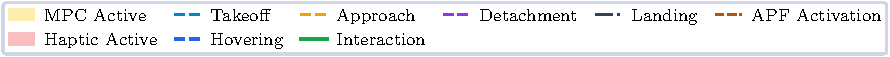
\includegraphics[width=\linewidth]{Immagini/Capitolo7/Experiments/Mission/phases_legend.pdf}
\end{subfigure}
\begin{subfigure}[b]{0.49\textwidth}
    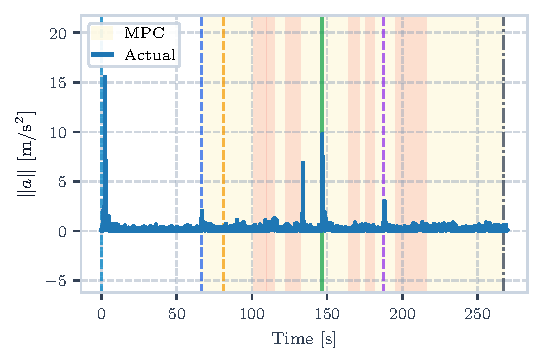
\includegraphics[width=\linewidth]{Immagini/Capitolo7/Experiments/Mission/DERIVATIVE_NORMS_norm_acc.pdf}
\end{subfigure}
\begin{subfigure}[b]{0.49\textwidth}
    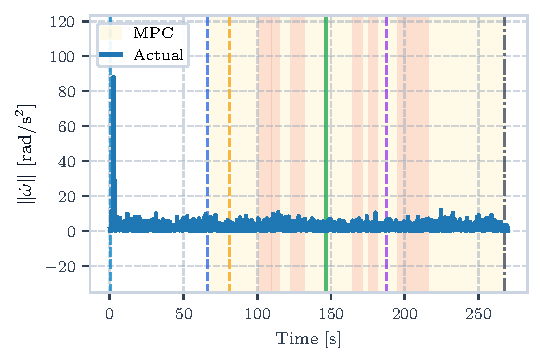
\includegraphics[width=\linewidth]{Immagini/Capitolo7/Experiments/Mission/DERIVATIVE_NORMS_norm_angacc.pdf}
\end{subfigure}
\begin{subfigure}[b]{0.49\textwidth}
    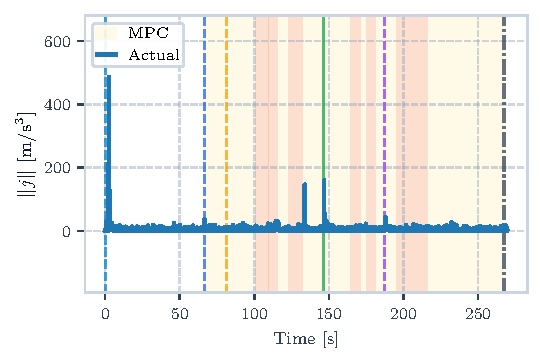
\includegraphics[width=\linewidth]{Immagini/Capitolo7/Experiments/Mission/DERIVATIVE_NORMS_norm_jerk.pdf}
\end{subfigure}
\begin{subfigure}[b]{0.49\textwidth}
    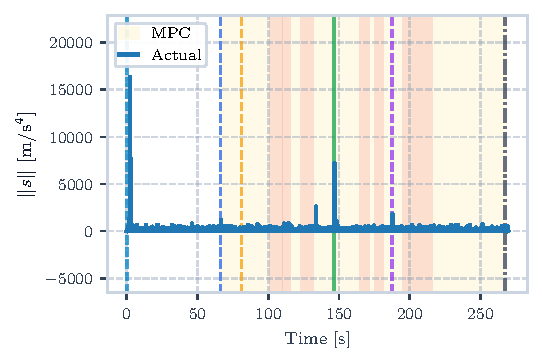
\includegraphics[width=\linewidth]{Immagini/Capitolo7/Experiments/Mission/DERIVATIVE_NORMS_norm_snap.pdf}
\end{subfigure}
\caption{Norms of higher-order dynamic derivatives recorded during the partial mission flight.}
\label{fig:hw_mission_derivative_norms}
\end{figure}
\justify
Figure~\ref{fig:hw_mission_derivative_norms} presents the dynamic derivative norms recorded during the mission flight. As in the teleoperation test, jerk and snap penalty terms were excluded from the cost function to preserve onboard computational resources. Even without explicit higher-order regularization, linear velocity remained strictly contained ($0.137\text{ m/s}$ RMS, $0.815\text{ m/s}$ maximum), and linear acceleration exhibited an RMS norm of $0.495\text{ m/s}^2$ ($15.533\text{ m/s}^2$ peak during abrupt phase step commands). The vehicle navigated between viewpoints without excessive oscillations.
Furthermore, no distance or camera FoV constraint violations occurred throughout the test ($s_r = 0.00\text{ m}$, $s_{\text{fov},h} = 0.00^\circ$, $s_{\text{fov},v} = 0.00^\circ$), with the APF generating a maximum peak repulsive force of $3.04\text{ N}$.

Looking at the control wrench components reported in Figure~\ref{fig:hw_mission_control_wrench}, the generated control actions remain smooth and well within the feasible actuation envelope throughout the flight. The total thrust $F_z$ averages $38.06\text{ N}$, with moderate variations during altitude reconfigurations and no saturation. In agreement with the previous test, the torque components are devoid of chattering, and $\tau_y$ continuously counterbalances the front camera pitch torque with a steady mean of $-0.18\text{ N}\cdot\text{m}$, further validating the real-world stability and robustness of the control outputs.

\begin{figure}[htbp]
\centering
\begin{subfigure}[b]{0.71\textwidth}
    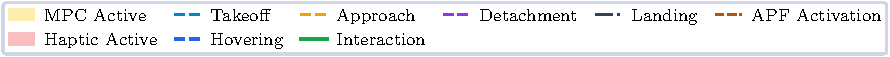
\includegraphics[width=\linewidth]{Immagini/Capitolo7/Experiments/Mission/phases_legend.pdf}
\end{subfigure}
\begin{subfigure}[b]{0.49\textwidth}
    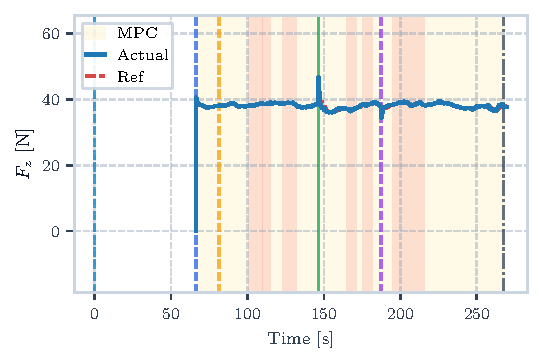
\includegraphics[width=\linewidth]{Immagini/Capitolo7/Experiments/Mission/CONTROL_WRENCH_force_z.pdf}
\end{subfigure}
\begin{subfigure}[b]{0.49\textwidth}
    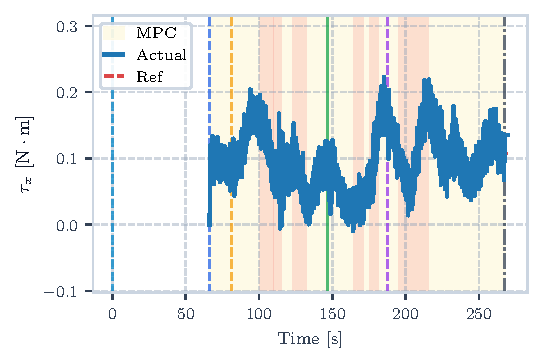
\includegraphics[width=\linewidth]{Immagini/Capitolo7/Experiments/Mission/CONTROL_WRENCH_torque_x.pdf}
\end{subfigure}
\begin{subfigure}[b]{0.49\textwidth}
    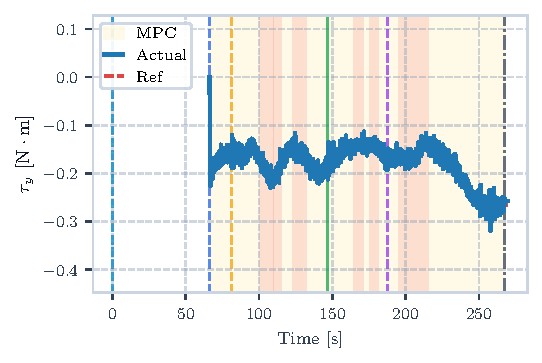
\includegraphics[width=\linewidth]{Immagini/Capitolo7/Experiments/Mission/CONTROL_WRENCH_torque_y.pdf}
\end{subfigure}
\begin{subfigure}[b]{0.49\textwidth}
    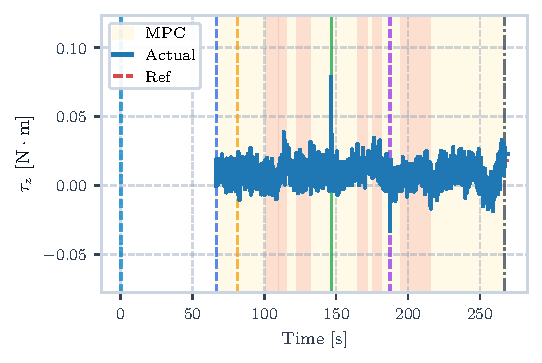
\includegraphics[width=\linewidth]{Immagini/Capitolo7/Experiments/Mission/CONTROL_WRENCH_torque_z.pdf}
\end{subfigure}
\caption{Control wrench components ($F_z, \tau_x, \tau_y, \tau_z$) commanded by the NMPC during the partial mission flight test.}
\label{fig:hw_mission_control_wrench}
\end{figure}
The complete set of performance metrics for the mission flight test is summarized in Table~\ref{tab:hw_mission_metrics}.
\begin{table}[htbp]
\centering
\small
\caption{Performance metrics and benchmark for the real-world partial cooperative mission flight test.}
\label{tab:hw_mission_metrics}
\begin{tabular}{lc}
\toprule
\textbf{Metric} & \textbf{Value} \\
\midrule
Nominal Control Frequency ($1/T_s$) & \SI{100}{\hertz} \\
Mean Solver Solve Time & \SI{2.29}{\milli\second} (CPU Load: \SI{22.9}{\percent}) \\
99th Percentile Solve Time & \SI{6.02}{\milli\second} \\
Solver Overruns ($> \SI{10}{\milli\second}$) & \SI{0.06}{\percent} ($3 / 4762$) \\
\midrule
Radial Distance RMS / Max Error ($r$) & \SI{0.214}{\meter} / \SI{0.768}{\meter} \\
Azimuth Angle RMS / Max Error ($\beta$) & \ang{8.58} / \ang{23.07} \\
Elevation RMS / Max Error ($z_{rel}$) & \SI{0.082}{\meter} / \SI{1.040}{\meter} \\
Yaw Angle RMS / Max Error ($\psi$) & \ang{3.98} / \ang{25.30} \\
\midrule
Linear Velocity ($\|v\|$) RMS / Max & \SI{0.137}{\meter\per\second} / \SI{0.815}{\meter\per\second} \\
Angular Velocity ($\|\omega\|$) RMS / Max & \SI{0.113}{\radian\per\second} / \SI{1.688}{\radian\per\second} \\
Linear Acceleration ($\|a\|$) RMS / Max & \SI{0.495}{\meter\per\second\squared} / \SI{15.533}{\meter\per\second\squared} \\
\midrule
Max Distance Violation ($s_r$) & \SI{0.000}{\meter} \\
Max Horizontal FoV Violation ($s_{\text{fov},h}$) & \ang{0.00} \\
Max Vertical FoV Violation ($s_{\text{fov},v}$) & \ang{0.00} \\
Max Peak Repulsive Force ($\|F_{\text{rep}}\|_{\infty}$) & \SI{3.04}{\newton} \\
Mean One-Way Haptic Latency & \SI{59.28}{\milli\second} \\
\bottomrule
\end{tabular}
\end{table}

These experimental flight tests successfully demonstrate the feasibility and robustness of the embedded NMPC formulation and bilateral haptic teleoperation on real multirotor hardware under actual sensor noise, aerodynamic disturbances, and wireless communication latencies.
    \chapter{Conclusions and Future Works}
    \section{Conclusions}
In this thesis, an exocentric vision framework has been deployed for a contact inspection task, through a cooperative dual-UAV \textit{Shared Control} architecture . The framework decouples the overall mission into separate roles: an Inspection UAV designed for safe physical contact, and an Observer UAV tasked with providing an "optimal" and active Point of View (PoV) for a human operator via a bilateral haptic teleoperation interface.
\\To ensure visual tracking and situational awareness, the Observer UAV is governed by a Nonlinear Model Predictive Controller (NMPC) operating in relative cylindrical coordinates. By continuously regulating relative horizontal distance, relative elevation, and camera heading, the optimal solver guarantees that the target vehicle remains centered within the camera Field of View. Furthermore, the explicit penalization of higher-order dynamic derivatives (jerk and snap) within the cost function effectively minimizes aggressive camera motions and operator motion sickness. On the interaction side, the Inspection UAV incorporates a dynamic admittance filter that translates measured or estimated contact forces into compliant reference displacements, preventing mechanical bouncings and ensuring stable physical coupling against vertical structures.
\\A shared teleoperation architecture based on the Novint Falcon haptic device bridges the human operator with the multi-agent system. The device maps pilot inputs to relative viewpoint adjustments while sending tactile safety cues through an Artificial Potential Field (APF). Exponential repulsive forces prevent the operator from violating the minimum inter-UAVs safety distance or driving the target outside the optical aperture.
\\The system has been validated both in high-fidelity Software-In-The-Loop (SITL) simulations and through physical flight experiments. Embedded real-world tests executed onboard a custom octocopter powered by a LattePanda companion computer demonstrated the computational feasibility of the framework: the NMPC solver executed with an average solve time of $2.57\text{ ms}$ at $100\text{ Hz}$, with overruns limited to $0.08\%$. Physical flight tests further validated the Shared Control framework through the bilateral haptic interface: despite a mean one-way wireless communication latency of $45.56\text{ ms}$, the tactile feedback remained completely responsive. When human inputs drove the vehicle towards the minimum standoff distance ($r_{\min} = 1.0\text{ m}$) or the vertical camera FoV limits, the APF triggered repulsive forces up to the $15\text{ N}$ saturation limit, reliably repelling the human operator and restoring a safe observation geometry.
\section{Future Works}
Despite good results already obtained, several directions can be pursued to improve and further advance this research:
\begin{itemize}
    \item \textbf{Simultaneous Dual-UAV Real Flights:} Extending the physical experimental campaign to concurrently deploy both custom UAV platforms in the flight arena, validating the complete cooperative mission pipeline including dynamic contact in hardware.
    \item \textbf{Vision-Based Onboard Target Detection:} Replacing the external motion capture system (OptiTrack) with onboard visual detection algorithms running on the camera payload, closing the perception-action loop entirely onboard.
    \item \textbf{Obstacle Avoidance:} Augmenting the NMPC formulation and the haptic APF with static or dynamic obstacle avoidance constraints to handle complex scenarios with static and moving obstacles.
    \item \textbf{Adaptive Admittance Control:} finding a mathematical definition of Optimal Point Of View, at least for this task.
\end{itemize}

    \appendix 
    \chapter{Implementation details}
    \label{app:implementation_details}
This appendix provides an overview of the low-level software implementation and configurations used for the control algorithms discussed in Chapter 5. It details the execution pipeline of the Non-linear Model Predictive Control (NMPC), the discrete-time formulation of the admittance filter, and the kinematic mapping logic embedded within the haptic interface.

\section{Observer Drone: Real-Time NMPC Implementation}
The active visual tracking task relies on the Non-linear Model Predictive Control (NMPC) scheme formalized in Chapter 4. Solving a continuous optimal control problem online on a flying platform requires a highly efficient and deterministic execution loop. To achieve real-time feasibility both in simulation and on real onboard companion computer, the mathematical modeling and discretization were performed using the CasADi symbolic framework, while the open-source package Acados was utilized to generate optimized and allocation-free C code for the solver. 

\noindent The optimization algorithm runs within a dedicated ROS 2 node governed by a wall-timer, executing at a fixed frequency $f_s$. Operating an NMPC online introduces significant computational and timing challenges; therefore, specific robustness mechanisms and solver options were implemented.

\subsection{Acados Solver Pipeline: ERK, SQP-RTI and HPIPM}
To guarantee deterministic execution within the control cycle on the onboard companion computer, the optimization problem is solved using the \texttt{acados} package. The solver combines several numerical strategies to ensure fast execution:
\begin{itemize}
    \item \textbf{ERK Discretization and Linearization:} The continuous non-linear quadrotor model is discretized over the horizon using an Explicit Runge-Kutta 4th-order (ERK4) integrator. At each step, the dynamic constraints are linearized around the current predicted trajectory, computing the state and input sensitivities via automatic differentiation.
    \item \textbf{Gauss-Newton Hessian Approximation:} Exploiting the Nonlinear Least Squares (NLS) form of the tracking cost defined in Chapter 4, \texttt{acados} approximates the Hessian of the Lagrangian through the Gauss-Newton method:
    \begin{equation}
        \mathbf{H}_k \approx \mathbf{J}_k^\top \mathbf{W} \mathbf{J}_k,
    \end{equation}
    where $\mathbf{J}_k$ is the Jacobian of the residual vector. This avoids evaluating computationally expensive second-order model derivatives while guaranteeing a positive semi-definite Hessian.
    \item \textbf{Real-Time Iteration (SQP-RTI):} Instead of iterating until full numerical convergence, the solver performs a single Sequential Quadratic Programming (SQP) iteration per timestep using the Real-Time Iteration (RTI) scheme. The computation is split into two phases:
    \begin{enumerate}
        \item \textit{Preparation Phase:} Executed in the background before the state measurement is available. The system equations are linearized, and the multi-stage Quadratic Program (QP) is prepared and partially condensed.
        \item \textit{Feedback Phase:} As soon as the updated state estimate is received from odometry, it is used as the initial condition constraint. The QP is solved immediately, and the first optimal control input $\mathbf{u}_0 = [F_z, \boldsymbol{\tau}^\top]^\top$ is published to the PX4 autopilot, minimizing feedback delay.
    \end{enumerate}
    \item \textbf{QP Subproblem Solver (HPIPM):} The resulting linearized QP is solved using \texttt{HPIPM} (High-Performance Interior Point Method) over the \texttt{BLASFEO} linear algebra library. A partial condensing approach is applied to balance sparsity and matrix dimensions. The QP solver is configured in \texttt{SPEED} mode with a maximum of 15 interior-point iterations, strictly bounding the worst-case execution time well below $10\text{ ms}$.
\end{itemize}

\subsection{Online disturbance compensation via MBE}
A fundamental implementation detail of the control node is the real-time integration of the Momentum-Based Estimator (MBE). The estimator algorithm executes synchronously with the 100 Hz control loop. At each iteration, the currently estimated external force $F_{ext}$ and torque $\tau_{ext}$ are passed dynamically to the CasADi model via the Acados parameter vector (\texttt{model.p}). 

\noindent Basically, instead of expanding the state vector of the optimization problem, which would heavily increase the computational effort, the disturbances are treated as online-updatable model parameters.

\subsection{Warm-Start and Delay Compensation}
To minimize the computational effort and reduce the number of Sequential Quadratic Programming (SQP) iterations required at each cycle, a warm-starting technique is employed. At the beginning of each 10 ms control loop, the solver is initialized with the optimal state and input trajectories computed during the previous timestep. 

\noindent Despite the optimized C code, unexpected CPU loads or operating system scheduling can occasionally cause the solver execution time to exceed the 10 ms threshold. Applying an outdated control input would introduce a dangerous phase lag in the closed-loop system. To mitigate this, the node continuously measures the exact execution time of the Acados solver using high-resolution clocks. If the computation time exceeds $T_s$, the node automatically shifts the extracted optimal control array forward by the corresponding number of discrete steps, ensuring that the applied thrust and torques are strictly aligned with the current real-world time.

\subsection{Safe-Switch Logic}
As detailed in Section 5.3, the observer drone performs its initial takeoff relying on the native PX4 position controller, eventually switching to the NMPC direct actuation (thrust and torques). An aggressive switch between two different controllers can result in severe mechanical jerks, potentially destabilizing the drone.

\noindent To ensure a smooth transition, a safe-switch logic governs the MPC controller introduction. Upon reaching the hovering altitude, the NMPC solver is activated in the background, computing the optimal commands based on the current state, but without publishing them to the flight controller. Concurrently, the node subscribes to the \texttt{vehicle\_torque\_setpoint} topic to monitor the actuation currently commanded by the PX4 autopilot. 

\noindent The actual switch to Offboard direct actuation is authorized by the node only when both the scalar difference in thrust and the Euclidean norm of the difference in torques between the NMPC-computed commands ($T_{\text{NMPC}}$, $\tau_{\text{NMPC}}$) and the currently active PX4 outputs ($T_{\text{PX4}}$, $\tau_{\text{PX4}}$) fall below their respective predefined safety thresholds:
$$|T_{\text{NMPC}} - T_{\text{PX4}}| < \epsilon_{T} \quad \text{and} \quad \|\tau_{\text{NMPC}} - \tau_{\text{PX4}}\|_2 < \epsilon_{\tau}$$
where $\epsilon_{T} > 0$ and $\epsilon_{\tau} > 0$. This guarantees that all control variables are continuous at the exact moment of the handover, completely eliminating transient instability and altitude drops.

\section{Observer Drone: Disturbance Estimation}
There are several ways to en-robust a controller to model uncertainties and disturbances for a drone. The chosen approach relies on Momentum Based Estimator.
\subsubsection{Physical Principle and Model Decoupling}
The fundamental intuition behind the momentum-based observer is to isolate external disturbances by canceling out the known nominal dynamics of the system. Let's start focusing on linear forces; the same concepts can be extended on the angular torques. Recall from Eq.~\eqref{eq:quadrotor_model} that the translational dynamics can be expressed in terms of the linear momentum $\mathbf{p}_T = m \mathbf{v}$:
\begin{equation}
    \dot{\mathbf{p}}_T = m \dot{\mathbf{v}} = \mathbf{F}_{\text{thrust}} - m\mathbf{g} + \mathbf{F}_{ext},
\end{equation}
where $\mathbf{F}_{\text{thrust}} = \mathbf{R}(\mathbf{q}) \begin{bmatrix} 0 & 0 & F_z \end{bmatrix}^\top$ is the actual control force generated by the propellers rotated into the inertial (world) frame, $m\mathbf{g}$ is the gravitational force, and $\mathbf{F}_{ext}$ accounts for all unmodeled external forces.
\\An attempt to reconstruct $\mathbf{F}_{ext}$ from this equation would require computing the linear acceleration $\dot{\mathbf{v}}$. In practice, numerically differentiating velocity signals (or reading noisy onboard accelerometer data) introduces high-frequency noise from motor vibrations, making the resulting estimate unusable for closed-loop control.
\\Instead, the estimator handles numerical differentiation by operating on an integral principle. To this end, we define the \textit{nominal force} acting in the physical model as:
\begin{equation} \label{eq:F_nom}
    \mathbf{F}_{\text{nom}} = \mathbf{F}_{\text{thrust}} - m\mathbf{g} = \mathbf{R}(\mathbf{q}) \begin{bmatrix} 0 \\ 0 \\ F_z \end{bmatrix} - m\mathbf{g}.
\end{equation}
It is essential to clarify the physical distinction: $\mathbf{F}_{\text{thrust}}$ is the sole active control force commanded to the actuators, whereas $\mathbf{F}_{\text{nom}}$ represents the resultant of all known modeled forces acting on the drone (actuation thrust plus gravity). The true rate of change of momentum is thus:
\begin{equation}
    \dot{\mathbf{p}}_T = \mathbf{F}_{\text{nom}} + \mathbf{F}_{ext}.
\end{equation}
The key objective of the estimator is to \textit{cancel out the nominal dynamics} $\mathbf{F}_{\text{nom}}$, leaving only the influence of the unknown disturbance $\mathbf{F}_{ext}$.

\subsubsection{Observer Dynamics and Disturbance Estimation}
To achieve this cancellation, an auxiliary state $\mathbf{I}_T \in \mathbb{R}^3$ is introduced to accumulate the expected momentum. The observer integrates the known nominal force alongside the current residual estimate $\mathbf{r}_T$ (which tracks $\mathbf{F}_{ext}$):

\begin{align}
    \dot{\mathbf{I}}_T &= \mathbf{F}_{\text{nom}} + \mathbf{r}_T, \label{eq:mbe_trans_I} \\
    \dot{\mathbf{r}}_T &= \mathbf{K}_{1,T} \left( -\mathbf{r}_T + \mathbf{K}_{2,T} (\mathbf{p}_T - \mathbf{I}_T) \right), \label{eq:mbe_trans_r}
\end{align}
where $\mathbf{p}_T = m \mathbf{v}$ is the actual momentum obtained from smooth odometry.
By defining the momentum estimation error as $\mathbf{e}_p = \mathbf{p}_T - \mathbf{I}_T$, its time derivative evaluates to:
\begin{equation}
    \dot{\mathbf{e}}_p = \dot{\mathbf{p}}_T - \dot{\mathbf{I}}_T = (\mathbf{F}_{\text{nom}} + \mathbf{F}_{ext}) - (\mathbf{F}_{\text{nom}} + \mathbf{r}_T) = \mathbf{F}_{ext} - \mathbf{r}_T.
\end{equation}
Here: the nominal model dynamics $\mathbf{F}_{\text{nom}}$ (both propeller thrust and gravity) cancel out completely. What remains in the error dynamics is solely the discrepancy between the actual disturbance $\mathbf{F}_{ext}$ and its estimate $\mathbf{r}_T$. Equations~\eqref{eq:mbe_trans_I}--\eqref{eq:mbe_trans_r} yield a stable and damped second-order linear filter that drives $\mathbf{r}_T \to \mathbf{F}_{ext}$ as a low-pass filter. The diagonal gain matrices $\mathbf{K}_{1,T}$ and $\mathbf{K}_{2,T}$ are tuned to obtain a desired settling time and critical damping ratio.
\\An identical decoupled architecture is applied to the rotational channel. In terms of angular momentum $\mathbf{p}_R = \mathbf{J} \boldsymbol{\omega}$ in the body frame, the rotational dynamics are governed by:
\begin{equation}
    \dot{\mathbf{p}}_R = \mathbf{J} \dot{\boldsymbol{\omega}} = \boldsymbol{\tau} - \boldsymbol{\omega} \times (\mathbf{J} \boldsymbol{\omega}) + \boldsymbol{\tau}_{ext},
\end{equation}
where $\boldsymbol{\tau}$ is the control torque vector commanded to the propellers, $\boldsymbol{\omega} \times (\mathbf{J} \boldsymbol{\omega})$ is the gyroscopic/Coriolis torque, and $\boldsymbol{\tau}_{ext}$ is the unmodeled disturbance torque. 
The known nominal torque predicted by the rotational model is defined as:
\begin{equation} \label{eq:tau_nom}
    \boldsymbol{\tau}_{\text{nom}} = \boldsymbol{\tau} - \boldsymbol{\omega} \times (\mathbf{J} \boldsymbol{\omega}).
\end{equation}
The rotational observer evolves according to:
\begin{align}
    \dot{\mathbf{I}}_R &= \boldsymbol{\tau}_{\text{nom}} + \mathbf{r}_R, \label{eq:mbe_rot_I} \\
    \dot{\mathbf{r}}_R &= \mathbf{K}_{1,R} \left( -\mathbf{r}_R + \mathbf{K}_{2,R} (\mathbf{p}_R - \mathbf{I}_R) \right), \label{eq:mbe_rot_r}
\end{align}
which cancels out the nominal control and Coriolis torques, allowing the residual $\mathbf{r}_R$ to converge smoothly to $\boldsymbol{\tau}_{ext}$.


\section{Inspection Drone: Admittance Filter Node (Simulation)}
To enable safe physical interaction and compliance when touching the environment, the simulated Inspection Drone relies on an admittance control architecture.

\noindent The admittance filter is implemented as a dedicated Python ROS 2 node operating at a deterministic rate of 100 Hz. Its main purpose is to shape the vehicle's dynamic behavior, translating external contact forces, measured by the tip-mounted 1D force sensor, into compliant motion references. 

\subsection{Discrete-Time Implementation and Low-Pass Force Filtering}
The continuous second-order mass-damper-spring admittance model, defined in Chapter 3 to govern the virtual interaction dynamics, is discretized using a forward Euler integration scheme. At each control step $k$, the raw force measurements $F_{\text{raw}}[k]$ received from the sensor topic are processed using a discrete-time low-pass filter (EMA-Exponential Moving Average) to attenuate high-frequency noise and mechanical vibrations:
$$F_{\text{filtered}}[k] = \alpha F_{\text{raw}}[k] + (1 - \alpha) F_{\text{filtered}}[k-1]$$
where $\alpha \in (0, 1]$ represents the filter smoothing factor. 

\noindent The resulting pre-processed interaction force drives the acceleration and velocity updates of the virtual mass. The filtered position offset is then imposed over the nominal trajectory references before being published as a compliant target.

The output compliant coordinates ($x_c, y_c, z_c$) are continuously published via the \texttt{TrajectorySetpoint} message to the top-level PX4 position cascade.

\section{Haptic Teleoperation Interface}
\subsection{Coordinate Frame Transformation and Kinematic Mapping}
The Novint Falcon needed an alignment of coordinate systems to be employed in this architecture. The device operates within its own Cartesian workspace, whereas the ROS 2 control architecture relies on standard conventions (Front-Left-Up, FLU, or East-North-Up, ENU). 
For this reason, by denoting with $\mathbf{p}_\text{haptic}$ the position of end effector in haptic frame, a rotation matrix $\mathbf{R}_{\text{haptic}}^{\text{flu}}$ is applied directly within the interface node to bring in drone body frame (see figure \ref{fig:haptic_render}):
\begin{equation*}
    \mathbf{p}_{\text{flu}} = \mathbf{R}_{\text{haptic}}^{\text{flu}} \mathbf{p}_{\text{haptic}},    
\end{equation*}
where
\begin{equation*}
     R_{haptic}^{flu}=\begin{bmatrix}
    -1 & 0 & 0 \\ 0 & -1 & 0 \\ 0 & 0 & -1
\end{bmatrix}
\end{equation*}
This transformation maps the device workspace safely to the operational boundaries of the aerial vehicles, preventing operator from mirrored control responses.

\noindent Furthermore, since the physical workspace of the Novint Falcon is constrained to a limited volume, a kinematic scaling factor is applied.

\noindent The exact mapping strategy strictly depends on the active teleoperation target. When commanding the Inspection Drone, the device acts essentially as a velocity joystick: the scaled haptic displacements are mapped directly into Cartesian velocity setpoints ($\mathbf{v}_{\text{ref}}$) for the top-level trajectory generator. 

\noindent Differently, when controlling the Observer Drone, the NMPC formulation requires maintaining a visual lock on the target. In this mode, the haptic inputs are mapped to dynamically modify the cylindrical references (i.e., radial distance $\rho$, angular phase $\phi$, and relative height $z$) governing the camera's viewpoint. This allows the operator to intuitively orbit or approach the target, while the optimal solver handles the underlying vehicle stabilization and decides for target positioning inside the camera image plane.

\subsection{Force Saturation}
To protect the mechanical actuators of the Novint Falcon and ensure operator safety, the output force feedback vector $\mathbf{F}_{\text{haptic}}$ dispatched to the device is strictly saturated:
$$\mathbf{F}_{\text{haptic}} = \text{sat}\left(\mathbf{F}_{\text{computed}}, -\mathbf{F}_{\text{max}}, \mathbf{F}_{\text{max}}\right)$$
where $\mathbf{F}_{\text{max}}$ represents the maximum safe operational force threshold (typically capped at $\pm 10$ N based on the physical limits of the device). This guarantees a comfortable, bounded, and completely stable haptic experience for the human pilot throughout the mission phases.
    \printbibliography
\end{document}